
\documentclass[a4paper]{article}\usepackage[]{graphicx}\usepackage[]{color}
%% maxwidth is the original width if it is less than linewidth
%% otherwise use linewidth (to make sure the graphics do not exceed the margin)
\makeatletter
\def\maxwidth{ %
  \ifdim\Gin@nat@width>\linewidth
    \linewidth
  \else
    \Gin@nat@width
  \fi
}
\makeatother

\definecolor{fgcolor}{rgb}{0.345, 0.345, 0.345}
\newcommand{\hlnum}[1]{\textcolor[rgb]{0.686,0.059,0.569}{#1}}%
\newcommand{\hlstr}[1]{\textcolor[rgb]{0.192,0.494,0.8}{#1}}%
\newcommand{\hlcom}[1]{\textcolor[rgb]{0.678,0.584,0.686}{\textit{#1}}}%
\newcommand{\hlopt}[1]{\textcolor[rgb]{0,0,0}{#1}}%
\newcommand{\hlstd}[1]{\textcolor[rgb]{0.345,0.345,0.345}{#1}}%
\newcommand{\hlkwa}[1]{\textcolor[rgb]{0.161,0.373,0.58}{\textbf{#1}}}%
\newcommand{\hlkwb}[1]{\textcolor[rgb]{0.69,0.353,0.396}{#1}}%
\newcommand{\hlkwc}[1]{\textcolor[rgb]{0.333,0.667,0.333}{#1}}%
\newcommand{\hlkwd}[1]{\textcolor[rgb]{0.737,0.353,0.396}{\textbf{#1}}}%

\usepackage{framed}
\makeatletter
\newenvironment{kframe}{%
 \def\at@end@of@kframe{}%
 \ifinner\ifhmode%
  \def\at@end@of@kframe{\end{minipage}}%
  \begin{minipage}{\columnwidth}%
 \fi\fi%
 \def\FrameCommand##1{\hskip\@totalleftmargin \hskip-\fboxsep
 \colorbox{shadecolor}{##1}\hskip-\fboxsep
     % There is no \\@totalrightmargin, so:
     \hskip-\linewidth \hskip-\@totalleftmargin \hskip\columnwidth}%
 \MakeFramed {\advance\hsize-\width
   \@totalleftmargin\z@ \linewidth\hsize
   \@setminipage}}%
 {\par\unskip\endMakeFramed%
 \at@end@of@kframe}
\makeatother

\definecolor{shadecolor}{rgb}{.97, .97, .97}
\definecolor{messagecolor}{rgb}{0, 0, 0}
\definecolor{warningcolor}{rgb}{1, 0, 1}
\definecolor{errorcolor}{rgb}{1, 0, 0}
\newenvironment{knitrout}{}{} % an empty environment to be redefined in TeX

\usepackage{alltt}

%--- Load packages. 
\usepackage{amssymb}
\usepackage{amsmath}
\usepackage{framed}
%\usepackage{textcomp}

% for permil
\usepackage{wasysym}

\pagestyle{empty}


% avoid ugly indentation of paragraphs
\usepackage{parskip}
\usepackage{graphicx}

% open sans font
%\usepackage[default,osfigures,scale=0.95]{opensans}
\usepackage{newtxtext}
\usepackage{newtxmath}

% subfolder with the figures (within manuscript/)
\graphicspath{ {./figures/} }

% for author affiliations
\usepackage{authblk}

%allows inline citations
\usepackage[round]{natbib}
\bibliographystyle{plainnat}
%include bib in TOC
\usepackage[nottoc]{tocbibind}

% use for quotations
\usepackage{csquotes}

% for degree symbol
\usepackage{gensymb}

% for line numbers
\usepackage{lineno}

% margin size
\usepackage{geometry}
\geometry{verbose,tmargin=3cm,bmargin=3cm,lmargin=3cm,rmargin=3cm}

% for bibtex
% \usepackage{authordate1-4}
% \bibliographystyle{authordate1}

%allows subscripts in text mode
\usepackage{fixltx2e}

%allows rotation of table??
\usepackage{rotating} 

%allows alignment of caption to the left
\usepackage{caption}
\captionsetup[table]{singlelinecheck=false}

%allows not italic greek letters
\usepackage{textgreek}

%centers different heading styles (look at package detail for font info, etc)
\usepackage{sectsty}
  \chapterfont{\centering}
  \sectionfont{\centering}
  
%set page numering to roman and then change once chapters start  
\pagenumbering{roman}  

% subfolder with the figures (within manuscript/)
\graphicspath{ {./pdfs/} }



%--------------------------------------------------------------------------------------------%
\IfFileExists{upquote.sty}{\usepackage{upquote}}{}
\begin{document}




%--------------------------------------------------------------------------------------------%

\begin{titlepage}
    \begin{center}
        \vspace*{1cm}
        
        \huge
        \textbf{Resource allocation in Eucalpytus}
        
        \vspace{3.5cm}
        
        \Large
        By\\
        
        \vspace{1cm}
        
        \LARGE
        \textbf{Courtney Campany}
        
        \vfill
        
        A thesis submitted in fulfilment of the requirements \\
        for the degree of Doctor of Philosophy\\
        
        \vspace{2.5cm}
        
        
\includegraphics[width=0.4\textwidth]{WSU_HIE_Logo2.jpg}

        2015
        
    \end{center}
\end{titlepage}

%--------------------------------------------------------------------------------------------%
\section*{Acknowledgements}
\thispagestyle{empty}
        \vspace{1.5cm}
        I wish to thank Jesus and my mom yo

\clearpage
%--------------------------------------------------------------------------------------------%
\section*{}
\thispagestyle{empty}
    \begin{center}
      \vspace*{7cm}
        \LARGE
        \textbf{Statement of Authentication}
        \vspace{2.5cm}
        
        \normalsize
        The work presented in this thesis is, to the best of my knowledge and belief, original\\
        except as acknowledged in the text. I hereby declare that I have not submitted this\\
        material, either in full or in part, for a degree at this or any other institution.\\
        
    \end{center}
\clearpage
%--------------------------------------------------------------------------------------------%
\tableofcontents

\setcounter{page}{4}
\clearpage
%--------------------------------------------------------------------------------------------%
\section*{LIST OF TABLES}

\textbf{Table 2.1}. Responses of plant and leaf characteristics of \textit{Eucalyptus tereticornis} seedlings to soil volume treatments. Each value reflects the mean(standard error) for each treatment. Seedling mass and leaf {\textdelta}\textsuperscript{13}C values are from final harvest. Values of leaf starch, sugars, nitrogen and SLA represent overall means across measurement campaigns (n=6). Different letters represent significant differences between treatments. The volume effect P value represents the overall difference between seedlings with soil volume restriction and the control seedlings.
\\
\\
\textbf{Table 2.2}. Responses of root characteristics of \textit{Eucalyptus tereticornis} seedlings to soil volume treatments. Each value reflects the mean(standard error) for each treatment. All values are from the final harvest. Values for FRLD are only calculated for seedlings in containers as free seedlings have potentially unlimited soil volume to exploit. Different letters represent significant differences between treatments. The volume effect P value represents the overall difference between seedlings with soil volume restriction and the control seedlings, except for FRLD which represents only differences between seedlings in containers.
\\
\\
\textbf{Table 2.3}. Responses of leaf level gas exchange parameters of \textit{Eucalyptus tereticornis} seedlings to soil volume treatments. Each value reflects the mean(standard error) for each treatment. A\textsubscript{max}, R and g\textsubscript{s} are each measured at 25~$\degree$C. Values of A\textsubscript{max}, g\textsubscript{s} and g\textsubscript{1} represent overall means across measurement campaigns (n=6). R, J\textsubscript{max} and Vc\textsubscript{max} values are means of two measurement campaigns at beginning and end of gas exchange measurements. Different letters represent significant differences between treatments. The volume effect P value represents the overall difference between seedlings with soil volume restriction and the control seedlings.
\\
\\
\textbf{Table 2.S1}. Seedling growth model default parameters.
\\
\\
\textbf{Table 3.1}. \textit{Eucalyptus tereticornis} leaf morphological and physiological traits between full sun and shade leaves under ambient and elevated temperature treatments. Leaf mass per area, N\textsubscript{a}, {\textdelta}\textsuperscript{13}C, $\Psi\textsubscript{pd}$, $\Psi\textsubscript{l}$ and K\textsubscript{l} values represent treatment mean ($\pm$~1~standard error) across measurement campaigns (n=6). Values of Vc\textsubscript{max} and J\textsubscript{max} are treatment mean ($\pm$ 1 standard error) from AC\textsubscript{i} curves measured in each chamber at saturating light. Units of LMA and Leaf N\textsubscript{area} are g~m\textsuperscript{2}, K\textsubscript{l} is mmol~m\textsuperscript{-2}~s\textsuperscript{-1} MPa, WP is MPA and {\textdelta}\textsuperscript{13}C is \permil. Different letters represent significant differences between leaf type and temperature treatments. The P value represents the overall effect between each unique combination of leaf type and temperature treatment for each trait.
\\
\\
\textbf{Table 3.2}. Responses of \textit{Eucalyptus tereticornis} leaf gas exchange parameters for sun and shade leaves under ambient and elevated temperature treatments. Each value reflects the mean ($\pm$~1~standard error) for each treatment across gas exchange campaigns (n=6). Units for A and E are {\textmugreek}mol~m\textsuperscript{-2}~s\textsuperscript{-1}, for g\textsubscript{s} and g\textsubscript{m} are mol~m\textsuperscript{-2}~s\textsuperscript{-1} and for VPD are kPa. Different letters represent significant differences between leaf type, light environment and temperature treatments. The P value represents the overall effect between each unique combination of leaf type, light environment and temperature treatment for each parameter.
\\
\\
\textbf{Table 4.1}. Final harvest C mass of above and belowground tissues, cumulative aboveground tree C uptake (F\textsubscript{c,T}) and specific leaf area (SLA). Each value represents the mean ($\pm$~1 standard error) for each treatment combination. Units for C mass and F\textsubscript{c,T} are g~C, while SLA are cm\textsuperscript{2}~g\textsuperscript{-1}. For each variable, different letters represent significant differences between treatments from the overall model which includes CO\textsubscript{s} * drought interactions. P values represent overall differences of CO\textsubscript{s} or drought main effects and the CO\textsubscript{s} * drought interaction.
   
\addcontentsline{toc}{section}{LIST OF TABLES}       
\clearpage
%--------------------------------------------------------------------------------------------%
\section*{LIST OF FIGURES}

\textbf{Figure 2.1}. Soil volume treatment means $\pm$~standard error of height growth (a), diameter growth (b), and interpolated seedling leaf area (c) measured weekly of \textit{Eucalyptus tereticornis} seedlings across the experiment duration in 2013.
\\
\\
\textbf{Figure 2.2}. Daily maximum and minimum temperature (a), total daily PPFD (b), and daily maximum vapour pressure deficit (c) across the experiment duration in 2013.
\\
\\
\textbf{Figure 2.3}. Soil volume treatment means of biomass partitioning to leaves, stems, and roots at harvest (a), bi-variate relationships between mass allocation to leaves and stems + roots (b) and leaf mass as a function of fine root biomass with $\pm$~standard error (c). For (b) lines represent standardized major axis fitting of the log-transformed allometric relationships of leaf mass fraction by treatment. For (c) the dashed line is the 1:1 relationship and the solid line represents the significant log-log model fit (R\textsuperscript{2} = 0.82) with equation: log(x) = 0.983(log(y)) - 0.036.
\\
\\
\textbf{Figure 2.4}. Soil volume treatment means $\pm$~standard error, across all measurement campaigns (n = 6), of light saturated rates of photosynthesis at 25~$\degree$C. Different letters represent significant differences between treatments.
\\
\\
\textbf{Figure 2.5}. Photosynthetic capacity, on a leaf mass basis, as a function of accumulation of leaf starch (a) and leaf nitrogen content without TNC (b). Colors represent bins levels (n = 5) of both leaf starch and nitrogen grouped from low to high.  Lines represents predictions, for each bin level, from the linear mixed effects model equation of A\textsubscript{mass} as a function of starch and nitrogen. The marginal R\textsuperscript{2} (fixed effects only) was 0.37 and the conditional R\textsuperscript{2} (fixed and random effects) was 0.48 for the complete model.
\\
\\
\textbf{Figure 2.6}. Total carbon mass for harvested and modeled seedlings versus predicted total carbon gain after 120 days (a) and  reductions in final seedling carbon mass, both modeled and observed, as a function of the reduction in leaf photosynthesis across treatments (b). For (a) the dashed 1:1 identifies the difference between net total leaf carbon gain and gross seedling production. For (b) both seedling carbon mass and daily carbon assimilation were first scaled to the free seedling control.
\\
\\
\textbf{Figure 2.S1}. Sensitivity testing of seedling growth model to different carbon allocation strategies including; constraints of leaf mass fraction to treatment specific final harvest values (a) and increases in respiration of non-leaf tissue components by 50~\% (b). Open and filled symbols represent default model and harvest values, while shaded symbols represent model sensitivity to each scenario by soil volume treatment. Both seedling carbon mass and daily carbon assimilation were first scaled to the free seedling control.
\\
\\
\textbf{Figure 3.1}. Bars represent the local light environment for sun and shade leaves during six gas exchange campaigns from October 2013 to April 2014. Means $\pm$~1 standard error represent integrated PPFD, measured with a ceptometer, at the canopy height of each selected leaf. Each date represents the starting date for each measurement campaign. Points represent the mean ($\pm$~1 standard error) daily maximum air temperature during each campaign period.
\\
\\
\textbf{Figure 3.2}. (a) AC\textsubscript{i} curves for sun and shade leaves at elevated (ET) and ambient (AT) temperature treatments. AC\textsubscript{i} curves were measured once on all trees, in February 2014, at 25~$\degree$C and at saturating light (1800~{\textmugreek}mol~m\textsuperscript{-1}~s\textsuperscript{-1}). (b) The relationship between Vc\textsubscript{max} and mean leaf N\textsubscript{a} for each chamber, including sun leaves and shade leaves at low light. (c) The relationship between A\textsubscript{n} and leaf N\textsubscript{a} for sun and shade leaves measured under their ambient light and temperature conditions. For (b,c) the dashed line represents the significant linear model fit for all leaves, with a marginal and conditional R\textsuperscript{2} of 0.28 and 0.35 for (b) and 0.24 and 0.33 for (c).
\\
\\
\textbf{Figure 3.3}. The response of A to g\textsubscript{s} (a) and g\textsubscript{m} (b) for sun leaves measured at high light and shade leaves measured at both low and high light under their respective elevated and ambient temperature treatments. Lines represent either smoothed regressions from a generalized additive model fit (a) or linear model fits (b). Grey areas are 95\% confidence intervals from the mean.
\\
\\
\textbf{Figure 3.4}. The mean $\pm$~1 standard error of g\textsubscript{s} (a), g~\textsubscript{m} (b) and A\textsubscript{n} (c) of sun leaves and shade leaves at both low and high light pooled across six measurement dates.
\\
\\
\textbf{Figure 3.5}. (a) Response of instantaneous transpiration efficiency (ITE) to VPD for sun leaves and shade leaves at both low and high light with elevated and ambient temperature treatments. (b) The relationship between leaf {\textdelta}\textsuperscript{13}C and leaf N\textsubscript{a} for sun leaves at high light and shade leaves at low light. For (a) VPD is the leaf to air pressure difference inside the gas exchange cuvette and lines represent predictions from the optimal ITE model with a g\textsubscript{1} value for each leaf type and treatment. For (b) the dashed line represents the significant linear model fit for all leaves with a marginal and conditional R\textsuperscript{2}~=~ of 0.41 and 0.45, respectively.
\\
\\
\textbf{Figure 3.6}. Relationship between the observed discrimination of \textsuperscript{13}CO\textsubscript{2} measured during photosynthesis and measured C\textsubscript{i}/C\textsubscript{a} for sun leaves measured at high light and shade leaves measured at both low and high light. The solid line represents the theoretical line for C3 plants from \citet{evans1986carbon}.
\\
\\
\textbf{Figure 3.7}. The mean $\pm$~1 standard error of intercellular CO\textsubscript{2} concentration (a), CO\textsubscript{2} concentration in the chloroplasts (b) and CO\textsubscript{2} drawdown from substomatal cavities to sites of carboxylation of sun leaves and shade leaves at both low and high light.
\\
\\
\textbf{Figure 3.S1}. Daily maximum and minimum temperature (a) and total daily PPFD (b) for each chamber across the experiment duration.
\\
\\
\textbf{Figure 3.S2}. Photosynthetic CO\textsubscript{2} response (AC\textsubscript{c}) curves for sun and shade leaves at elevated and ambient temperature treatments. C\textsubscript{c} values were predicted with g\textsubscript{m}, thus curves represent chloroplastic photosynthetic parameters at 25~$\degree$C and saturating light (1800~{\textmugreek}mol~m\textsuperscript{-1}~s\textsuperscript{-1}). 
\\
\\
\textbf{Figure 3.S3}. Response of A (a), g\textsubscript{m} (b) and C\textsubscript{i}-C\textsubscript{c} to leaf temperature for sun leaves and shade leaves at low and high light. Shaded symbols represents each monthly measurement campaign. Solid lines, colored by leaf and light type, are fitted line for the relationship with each parameter and leaf temperature across all measurement campaigns. All parameters with no relationship are fitted with zero slope and the overall mean value for each treatment combination. Weak negative relationships with g\textsubscript{m} and increasing leaf temperature were detected with sun and shade leaves under their local light environment (R\textsuperscript{2}~=~0.16 and 0.08, respectively). 
\\
\\
\textbf{Figure 3.S4}. Response of VPD (a), g\textsubscript{s} (b) and C\textsubscript{a}-C\textsubscript{i} to leaf temperature for sun leaves and shade leaves at low and high light. Shaded symbols represents each monthly measurement campaign. Solid lines, colored by leaf and light type, are fitted line for the relationship with each parameter and leaf temperature across all measurement campaigns. All parameters with no relationship are fitted with zero slope and the overall mean value for each treatment combination. Leaf VPD inside the gas exchange cuvette was positively correlated with increasing leaf temperature for sun leaves and shade leaves at low and high light (R\textsuperscript{2}~=~0.73, 0.58 and 0.72, respectively).
\\
\\
\textbf{Figure 4.1}. Conceptual diagram depicting the major components of C flow among plant components including; uptake via photosynthesis, allocation to component tissues, tissue respiration and root exudation. Net aboveground C uptake (F\textsubscript{c,T}), shown in the shaded box, represents the flux of C measured within each WTC. With the WTC experimental design, total belowground C allocation (TBCA) is measured as the residual between F\textsubscript{c,T} and total aboveground C mass. 
\\
\\
\textbf{Figure 4.2}. Whole tree C mass as a function of cumulative aboveground C flux for each WTC tree. Values of cumulative aboveground net C flux were measured over the final eleven months of the experiment. Whole tree C mass represents the sum of bole, branch, leaf and root C mass from allometric estimates over the same time period. The dotted line is the 1:1 relationship and the solid line represents the significant overall linear model fit from the equation y = 0.56x + 878.2 (R\textsuperscript{2}~=~0.86).
\\
\\
\textbf{Figure 4.3}. Estimated canopy leaf area for each WTC tree over the final eleven months of the experiment (April 2008 to March 2009). Estimates are based on height growth, litterfall rates and two leaf area estimates following \citet{barton2012effects}. Color and line type distinguish the treatment combination for each WTC.
\\
\\
\textbf{Figure 4.4}. Treatment means of cumulative aboveground C flux as a function of mean daily canopy leaf area over the final eleven months of the experiment. The solid line represents the significant overall linear model fit (R\textsuperscript{2}~=~0.77) from the equation: y = 611.9x + 2791.2. Separate 95\% confidence intervals are shown for linear regression between F\textsubscript{c,T} and mean leaf area for aC\textsubscript{a} and eC\textsubscript{a} treatments.
\\
\\
\textbf{Figure 4.5}. Treatment means of C mass fractions of leaves (a), stems (branches+boles) (c) and roots (e) as a function of tree size, via whole tree C mass. Treatment means of C allocation to leaves (b) and stems (d) as a function of cumulative aboveground net C flux. Root C allocation could not be estimated as root turnover was not known. Values for C mass fractions are calculated from final harvest biomass totals. Values for C allocation are estimated from cumulative total aboveground net C flux over the final eleven months of the experiment. Solid lines represent overall linear model fit for leaf, stem and root mass fractions (R\textsuperscript{2} = 0.53,~0.26~and~0.01, respectively), as well as leaf and stem C allocation (R\textsuperscript{2}= 0.39, 0.01, respectively).
\\
\\
\textbf{Figure 4.6}. Cumulative aboveground net C flux and additive C allocation to individual tree components from 15 April 2008 to 16 March 2009. Each panel represents mean values for each treatment combination (n=3). Both aboveground net C flux and tissue C allocation where set to 0 on 15 April 2008 in order to track the allocation of C in daily time steps. Root C mass, predicted from the logarithmic relationship between above and belowground mass partitioning of pre-planting seedlings and harvested trees, is shown on the last date.
\\
\\
\textbf{Figure 4.7}. Treatment means $\pm$~1 standard error of cumulative aboveground net C flux, TBCA, and the residual belowground C flux (F\textsubscript{c,r}). Values of cumulative aboveground net C flux were measured over the final eleven months of the experiment. Values for TBCA are the residual between the cumulative C flux and total C mass aboveground estimated from allometric surveys over the same time period. Values for F\textsubscript{c,r} were calculated as the residual between TBCA and root C mass predicted on the last date of the eleven month period. 
\\
\\
\textbf{Figure 4.8}. Total belowground C allocation as a function of cumulative aboveground net C flux across the final eleven months of the experiment. Carbon mass aboveground was estimated from allometric surveys, interpolated on a daily time scale and then subtracted from the aboveground net C flux to quantify TBCA. Individual lines represent treatment means, with color and line type distinguishing treatment combinations.
\\
\\
\textbf{Figure 4.S1}.
Root mass as a function of shoot mass in \textit{Eucalyptus saligna} for potted seedlings harvested before planting of WTC trees (n=17) and WTC trees harvested after 2 years (n=12). Potted seedlings were grown in 25 l pots inside each WTC, while chamber [CO\textsubscript{2}] treatments conditions were maintained. The solid line represents the significant log-log model fit (R\textsuperscript{2} = 0.98) from the equation: log(x) = 0.77(log(y)) + 0.43.
\\
\\
\textbf{Figure 4.S2}.
Cumulative aboveground net C flux and additive C allocation of individual tree components from 2008-4-15 and 2009-3-16. Panels represent each individual WTC. Both aboveground net C flux and tissue C allocation where set to 0 on 2008-4-15 in order to track the allocation of C in daily time steps. Total root C mass, predicted from the log relationship between above and belowground mass partitioning of pre-planting seedlings and harvested trees, is shown on the last date.

\addcontentsline{toc}{section}{LIST OF FIGURES}      
\clearpage
%--------------------------------------------------------------------------------------------%
\section*{LIST OF ABBREVIATIONS}

\textit{A\textsubscript{n}}  Net leaf photosynthesis rate
\\
\\
A\textsubscript{c} Component specific biomass partitioning??
\\
\\
aC\textsubscript{a} Ambient CO\textsubscript{2} treatment
\\
\\
AC~i~ Photosynthetic CO\textsubscript{2} response curves 
\\
\\
A\textsubscript{max} Leaf net photosynthesis at saturating light and CO\textsubscript{2} concentration
\\
\\
A\textsubscript{sat} Leaf net photosynthesis at saturating light
\\
\\
AT  Ambient air temperature treatment
\\
\\
C Carbon
\\
\\
$[\textrm{CO\textsubscript{2}}]$ CO\textsubscript{2} concentration
\\
\\
C\textsubscript{ab} Aboveground standing crop C mass
\\
\\
C\textsubscript{day} Predicted daily carbon assimilation
\\
\\
C\textsubscript{i} Intercellular CO\textsubscript{2} concentration (or partial pressure)
\\
\\
C\textsubscript{c} Chloroplastic CO~\textsubscript{2} concentration (or partial pressure)
\\
\\
C\textsubscript{r,T}  Total C mass of roots
\\
\\
E Leaf transpiration
\\
\\
eC\textsubscript{a} Elevated CO\textsubscript{2} treatment
\\
\\
ET  Elevated air temperature treatment
\\
\\
FACE Free-air CO\textsubscript{2} enrichment experiments
\\
\\
F\textsubscript{c}  Net aboveground carbon uptake
\\
\\
F\textsubscript{c,r}  Residual belowground C flux
\\
\\
free  naturally planted
\\
\\
FRLD Fine root length density
\\
\\
g\textsubscript{s}  Stomatal conductance
\\
\\
g\textsubscript{m}  Mesophyll conductance
\\
\\
ITE Leaf level instantaneous transpiration efficiency
\\
\\
J\textsubscript{max} Maximum rate of photosynthetic electron transport 
\\
\\
K\textsubscript{l} Leaf-specific hydraulic conductance 
\\
\\
LA Leaf area
\\
\\
LMA Leaf mass per unit area
\\
\\
LMF Leaf mass fraction
\\
\\
N  Nitrogen
\\
\\
N\textsubscript{a} Leaf nitrogen on an area basis
\\
\\
N\textsubscript{f} TNC-free leaf nitrogen content
\\
\\
PPFD  Photosynthetic photon flux density
\\
\\
Q\textsubscript{10} Rate of change in respiration due to 10~$\degree$C increase in temperature
\\
\\
R Leaf dark respiration rates
\\
\\
RMF Root mass fraction
\\
\\
SLA Specific leaf area
\\
\\
SLA\textsubscript{f}  TNC-free Specific leaf area
\\
\\
SMF Stem mass fraction
\\
\\
TBCA Total belowground carbon allocation
\\
\\
TNC Total non-structural carbohydrate
\\
\\
TDL Tunable diode laser
\\
\\
Vc\textsubscript{max} Maximum rate of rubisco carboxylation 
\\
\\
VPD Vapour pressure deficit
\\
\\
VPDP Standard Vienna Pee Dee Belemnite
\\
\\
WUE Water-use efficiency
\\
\\
WTC Whole-tree chambers
\\
\\
{\textdelta}  Isotope discrimination
\\
\\
$\Delta$ Carbon isotope discrimination during C3 photosynthesis 
\\
\\
$\Psi\textsubscript{l}$ Midday leaf water potential
\\
\\
$\Psi\textsubscript{pd}$  Predawn leaf water potential
\\
\\
$\sigma$\textsubscript{s} Self shading parameter

\addcontentsline{toc}{section}{LIST OF ABBREVIATIONS}  
\clearpage
%--------------------------------------------------------------------------------------------%
\section*{ABSTRACT}

Plants must utilize external resources including light, CO\textsubscript{2}, water and mineral nutrients to support photosynthetic carbon (C) gain.  This photoassimilate is then allocated within the plant as the essential C resource for growth, maintenance and storage. Theory and observations suggest that C allocation and leaf physiology are optimized to maintain functional balance for external resource capture and to maximize C gain. However, the impacts of a changing climate may disrupt the proposed balance of C allocation between above and belowground pools. Variation in resource distribution and leaf physiology within tree canopies is also not fully understood, thus all canopy leaves may not follow theories of leaf optimal behavior. These unanswered questions regarding C uptake and fate of assimilated C inhibit our ability to precisely test the coordination between canopy photosynthesis and growth. To address these broad ecological questions, this PhD research utilized a diverse set of experiments which manipulated resource availability and climate factors on \textit{Eucalyptus} tree species. My goal was to measure aspects of resource allocation and C uptake across different scales, from leaf to whole tree, to improve physiological understanding of the processes which define tree growth and the sensitivity of these processes to changing environments.

\
First, I determined whether manipulations of soil volume would limit growth in \textit{Eucalyptus tereticornis} seedlings by disrupting the balance between source and sink activity. Seedlings were grown in a large range of container sizes and planted flush to the soil alongside naturally planted seedlings ('free'). Aboveground growth of seedlings in containers was negatively affected compared to free seedlings soon after the experiment started. Despite large reductions in growth across soil volume treatments, relative partitioning of mass to leaves, stems and roots was similar for all seedlings after 120 days. Leaf photosynthetic capacity decreased in containers compared to free seedlings, and was correlated to both leaf nitrogen (N) content and starch accumulation. Although belowground sink limitation resulted in a reduction of net leaf photosynthesis (\textit{A\textsubscript{n}}), a mass balance model concluded that these reductions were not large enough to explain observed growth responses. As \textit{A\textsubscript{n}} and growth were not tightly coordinated, the model predicted excess photosynthetic C not attributed to biomass in potted seedlings. Quantifying the fate of this excess C will be essential in evaluating feed-backs between sink strength and leaf C uptake in future studies.

\
Second, I investigated how light gradients within \textit{Eucalyptus tereticornis} tree canopies affect the distribution of resources that define photosynthetic capacity of sun and shade leaves. Trees were grown in climate-controlled  whole tree chambers under prevailing ambient and warmed (+3~$\degree$C) treatments and leaf gas exchange was coupled with online C isotope discrimination to measure *\textit{A\textsubscript{n}}, stomatal conductance (g\textsubscript{s}) and mesophyll conductance (g\textsubscript{m}) of sun and shade leaves. Photosynthesis rates were reduced by ca. 40~\% in shade leaves associated with a 75\% reduction in photosynthetically active radiation compared to sun leaves. Photosynthetic capacity (ca. 20\% lower Vc~max~ and J\textsubscript{max}) and leaf N were also lower in shade leaves than sun leaves however, g\textsubscript{s} was similar. Leaf C\textsubscript{i}, estimated from both leaf {\textdelta}\textsuperscript{13}C and gas exchange, was higher in shade leaves than sun leaves. Here, the optimization theory hypothesis that C\textsubscript{i} should be optimized throughout the canopy was rejected because water use efficiency was lower in shade leaves, compared to sun leaves. When light intensity was increased from low light to high light for shade leaves both g\textsubscript{s} and g\textsubscript{m} increased rapidly, leading to increases in \textit{A\textsubscript{n}} greater than sun leaves at the same high light environment. This rapid response of g\textsubscript{m} with light enables shade leaves to respond quickly to sunflecks and represents a new mechanism underpinning leaf gas exchange responses to light. This capacity of shade leaves to adjust their physiological behavior and increase C uptake when sunflecks occur likely plays significant role in whole tree C uptake for some tree species. These findings reveal that plant resources within a canopy may be distributed to utilize sunflecks and the dynamic physiological responses of shade leaves to altered light environments must be accounted for when up-scaling leaf level measurements to predict whole canopy C gain. 

\
Finally, I examined how net aboveground C uptake correlated to tree biomass growth and whether elevated $[\textrm{CO\textsubscript{2}}]$ and drought treatments altered C allocation patterns above or belowground in \textit{Eucalyptus saligna} trees. Trees were grown in climate-controlled whole tree chambers (WTCs) over a period of two years with interacting treatments of two [$[\textrm{CO\textsubscript{2}}]$ (380 ppm and 620 ppm) and two watering regimes (well-watered and a four-month drought). Additionally, we utilized a novel approach to calculate total belowground C allocation (TBCA) for each WTC as the residual between the aboveground net CO\textsubscript{2} uptake and aboveground C mass. Measured cumulative aboveground net C uptake correlated positively to whole tree C mass production and leaf area over the final eleven months of the experiment. Contrary to previous studies, cumulative TBCA was unaffected by either elevated CO\textsubscript{2} or drought treatments. As a fraction of total aboveground net C uptake, TBCA was also found to remain relatively stable across daily time steps for all trees. Increases in C allocation to leaves were detected in elevated CO\textsubscript{2} treatments, while the effects of a 4 month drought were negligible on C allocation in aboveground tissues.  These results reveal how climate change factors impact the investment of photosynthetic C in a \textit{Eucalyptus} tree species and provide evidence that belowground processes may not be as sensitive to global change factors as previously thought. 

\
In conclusion, this PhD research addressed diverse questions regarding resource allocation in \textit{Eucalyptus} tree species by linking leaf physiology to whole canopy C gain and allocation of photosynthetic C to whole tree growth. This study confirms that the distribution of photosynthetic resources constrain canopy C uptake, yet within canopy leaf physiology does not follow prevailing optimal theory. Results from this work reveal how quantifying the fate of photosynthetic C among tissue and ecosystem pools, beyond biomass production, is imperative to accurately assess the impacts of environmental change on tree productivity. This research offers critical empirical data needed to refine process based models which predict canopy C gain from rates of \textit{A\textsubscript{n}} and forest growth models where C allocation is represented. Ultimately, this work contributes valuable information regarding the physiological and growth responses of iconic \textit{Eucalyptus} tree species essential for reconciling the impacts of resource availability and global climate change on fragile Australian ecosystems and the productivity of *Eucalyptus* plantation forests. 

\addcontentsline{toc}{section}{ABSTRACT}      
\clearpage
%--------------------------------------------------------------------------------------------%
\section*{CHAPTER 1 \\ \mbox{ }\\ GENERAL INTRODUCTION}
\subsection*{OVERVIEW}

\subsubsection*{Resource allocation in plants}
Plants need to extract resources including light, CO\textsubscript{2}, water and mineral nutrients to support growth and reproduction. To accomplish this requires energy, appropriate tissues for uptake and a transport system to deliver resources to their required destination \citep{grace1997allocation}. The uptake of nutrients from roots is necessary for leaf growth. Leaves then fix the C, via net photosynthesis (\textit{A\textsubscript{n}}), required for growth of the entire plant. This assimilated C from source leaves, in the form of simple sugars, is in itself an essential C resource that must be allocated to the growth and maintenance of tissues or is diverted to a storage pool of carbohydrates. As a result, growth is driven by several simultaneous processes, including \textit{A\textsubscript{n}}, C investment among organs, resource acquisition and metabolic costs \citep{korner2006plant, fourcaud2008plant}. Gaining an understanding of the sensitivity of these processes to environmental change is crucial for predicting future terrestrial C cycling \citep{friedlingstein1999toward}, as there is currently little consensus on how C allocation should be modeled \citep{franklin2012modeling, de2014does}.

\subsubsection*{Resource allocation theory}
Theoretically, growth under resource limitation will be maximized when investment into the acquisition of any single resource from the environment leads to an equivalent increase in growth \citep{bloom1985resource}. The two critical assumptions of allocation theory are that the resource in question is in fixed supply and that allocation among competing functions is mutually exclusive \citep{bazzaz2000reproductive}. Thus, trade-offs between different tissue C sinks will exist as resources are invested within the plant. Allocation of newly acquired resources to different tissues will then affect subsequent rates of capture of CO\textsubscript{2} and soil resources \citep{shipley2002balanced}. In resource saturated environments plants should maximize growth by allocating resources to support leaf growth to increase C acquisition \citep{monsi2005factor}. Resource availability, however, is rarely saturated in natural ecosystems. As a result, shifts in allocation of external resources and assimilated C to different tissue or ecosystem components can occur.

\
Shifts in resource allocation within plants have led to two main theories regarding allocation strategies. First, the balanced growth hypothesis suggests that individual plant tissues should provide a \textquotesingle~balanced internal economy\textquotesingle~as each component supplies resources for the other \citep{davidson1969effect}. This functional equilibrium between tissues can then be adaptive if conditions limit \textit{A\textsubscript{n}} or soil nutrient uptake \citep{cannell1985attributes}, such that plants should allocate resources to the organ that is capturing the resource most limiting growth \citep{shipley2002balanced}. Changes in plant resource allocation are also theorized to be a function of allometric trajectories of plant development, independent of changes in nutrient supply \citep{muller2000effect}. In this strategy, investment into leaf mass increases with both stems and root, but not proportionally, as a greater allocation of biomass to the stem exists as a simple function of plant size \citep{zens2002sizing}. When constrained by ontogeny, plants are more likely to adjust tissue morphology, chemistry, metabolism or turnover to alter resource capture \citep{reich2002root}. 

\subsubsection*{Tree canopy resource gradients}
Incident PPFD declines exponentially with cumulative leaf area index from the top of the tree downward, creating steep light gradients within tree canopies \citep{monsi2005factor}. Leaf photosynthesis responds strongly and non-linearly to irradiance [@evans1995carbon]. As costs and limitations of light harvesting prevent plants from exposing all leaves to full sun [@niinemets2010review], it follows that a substantial portion of canopy C assimilation should occur in leaves with the highest exposure to light. Consequently, the distributions of resources required for \textit{A\textsubscript{n}} are partially defined by canopy light gradients. As the photosynthetic capacity of leaves is related to its N content \citep{field1986photosynthesis}, a larger investment in N to the upper canopy should yield a larger return from whole canopy C assimilation [@ellsworth1993canopy]. The supply of water also imposes limits photosynthetic C gain through direct limitations on leaf level physiology. The stomatal resistance to CO\textsubscript{2} uptake is a function of the balance between transpiration losses and leaf water potentials \citep{farquhar1982stomatal} and sun leaves frequently experience greater water limitations in the upper canopy \citep{sellin2008effects, niinemets2012optimization}. Thus, photosynthetic N investment in the upper canopy will be ineffective in enhancing \textit{A\textsubscript{n}} if water supply is insufficient \citep{niinemets2012optimization, peltoniemi2012co}. Overall, the allocation of soil resources within the canopy constrains leaf physiology and photosynthetic capacity, thereby regulating the efficiency of CO~2~ uptake.    

\subsubsection*{Fate of assimilated carbon}
Carbon allocation represents the fraction of net primary productivity distributed to different tissue components above and belowground. In trees, C allocation encompasses investment into tissue biomass production as well as fluxes including respiration, exudation and turnover rates \citep{litton2007carbon}. The fate of this assimilated C is regulated by the delicate balance between leaf C uptake (source) and the C sink strength of the different biomass pools. For example, the sensitivity of C source and sink activities to water and nutrient availability could lead to an imbalance between C supply and C used for tissue growth and respiration \citep{fatichi2014moving}. Additionally, imbalances between source and sink activity can lead to investment into carbohydrates synthesis as a transient C storage sink \citep{paul2001sink}.

\
As woody plants have competing tissue carbohydrate sinks, growth should principally depend on the allocation of leaf C assimilate among different sink organs \citep{kozlowski1992carbohydrate, lacointe2000carbon}. In response to changing environmental conditions, however, trees may adaptively shift tissue C allocation to balance growth, storage and C loss. Due to conservation of mass, it is theoretically possible to track the fates of this assimilate from leaf C uptake to their eventual destination in above and belowground pools. Although mass balance approaches can be used to quantitatively asses tree C allocation, few studies so far have been able to provide direct empirical measurements of C allocation among component pools \citep{klein2015}.

\subsubsection*{\textit{Eucalyptus} tree species as model for research}
Research on \textit{Eucalyptus} trees is ecologically important for Australia as it is the most dominant tree genus \citep{boland2006forest}. \textit{Eucalyptus} forests are the continent’s most common forest type, covering about three-quarters of Australia\textquotesingle s native forests (92 million hectares) and occurring in all but the continent\textquotesingle s driest regions \citep{ASOFR2013}. \textit{Eucalyptus} tree species are also economically important globally as they are commonly cultivated in plantations due to fast growth. Despite the fact that only a few \textit{Eucalyptus} species have natural ranges outside continental Australia \citep{pryor1981eucalyptus}, \textit{Eucalyptus} trees are grown in plantations in over 90 countries citep{booth2013eucalypt}. This is because \textit{Eucalyptus} species have been shown to exhibit both adaptive plasticity and genetic specialization to spatial variation in climate \citep{byrne2013adaptation}. Currently, the global plantation area of eucalypts totals nearly 20 million hectares, accounting for around 15~\% of the world\textquotesingle s total plantation forests \citep{IUFRO2015}. Consequently, this iconic Australian tree species is an excellent model to investigate strategies of resource allocation in trees facing global climate change.

\subsection*{CURRENT KNOWLEDGE GAPS}

\subsubsection*{Resource allocation in trees}
The distribution of assimilated C is a primary determinant of plant growth \citep{friedlingstein1999toward}, yet our knowledge of the mechanisms by which allocation is regulated is poor \citep{poorter2012biomass}. A key issue with drawing generalized conclusions about the plasticity of C allocation in trees is with the inconsistency in terminology used to define C allocation to specific tissue or ecosystem components \citep{litton2007carbon}. Biomass partitioning should not be confused with the allocation of newly fixed photosynthates to different organs, as the measured biomass at any time point represent the cumulative result of dynamic C allocation over time \citep{poorter2015does}. This dynamic C allocation includes not only tree parts such as leaves, stems and roots but also respiration, exudation, turnover and transient C storage pools. As C allocation integrates all of these processes, it is extremely difficult using current methods to assess C allocation in whole trees. Disentangling the effects of resource supply on plant C allocation patterns is often assessed across “snapshots” in time, which should be done with caution \citep{reich2002root}. This is because of plants have developmental shifts in biomass partitioning, independent of resource supply, as they age \citep{muller2000effect, poorter2015does}. Additionally, supplies of light and soil resources fluctuate continuously, making equilibrium with C allocation at any “snapshot” highly unlikely \citep{shipley2002balanced}.

As accurately measuring tree C allocation remains a difficult task, especially belowground, drawing conclusions that are applicable to whole plants or ecosystems remains a challenge. Currently, the representation of C allocation lags behind photosynthesis (\textit{A\textsubscript{n}}) in process-based forest models \citep{friedlingstein1999toward, franklin2012modeling, iversen2014terrestrial} and our understanding of how global change impacts C allocation is incomplete \citep{litton2007carbon, warren2012timing}. This knowledge gap of C allocation patterns in trees is of major concern due to the potential for forest ecosystems to sequester C in a changing climate. This deficiency requires more empirical data to derive basic principles that drive patterns of tree C allocation in changing environments. However, this will require novel experiments and approaches to better quantify shifts in C allocation above and belowground in future studies. 

\subsubsection*{Coupling of photosynthesis and tree growth}
On short timescales, \textit{A\textsubscript{n}} and respiratory losses may not correlate with growth because of tissue C storage pools. On longer timescales, however, they determine net plant C balance and must correlate to growth. This had led to the long standing debate over how strongly plant growth is controlled by either source or sink activity \citep{sweet1966role, korner2013growth}. Studies manipulating either source activity (CO\textsubscript{2} fumigation or defoliation) or sink activity (fruit removal, girdling or low growth temperatures) have not reached consensus when addressing this debate. This uncertainty arises from the difficulty in measuring the balance between C uptake and the fate of assimilated C among pools with long (biomass) or short (carbohydrate storage, respiration, exudation) retention times. When shifts in carbohydrate storage, tissue respiration or turnover rates occur, rates of C assimilation may not correlate with biomass production at a given time point \citep{rocha2006linking, litton2007carbon, gough2008multi}. To assess this balance will likely require integration of empirical and modelling approaches to assess leaf physiological and whole plant responses to manipulations of source-sink activity. To address this knowledge gap, new approaches are needed to test how interactions between source and sink activity affect the fate of assimilate C across different temporal scales. 

\subsubsection*{Within canopy resource utilization}
Due to the relationships between light, N and leaf photosynthetic capacity, it is commonly assumed that a limited availability of N should be distributed proportional to light availability within tree canopies. Observed canopy distribution of N is often less steep than optimal theory suggests, however, with shade leaves having more N than expected based on average light gradients [\citep{peltoniemi2012co}. Additionally, constraints on water distribution from the soil to the upper canopy may negatively impact the distribution of photosynthetic N to canopy light availability \citep{niinemets2012optimization, peltoniemi2012co}. Whether insufficient hydraulic supply results in the observed sub-optimal canopy N gradients has yet to be empirically tested. Assessing leaf C gain as a function of light availability is also made difficult by frequent light fluctuations within a canopy, via sunflecks. Sunflecks cause temporal variation in PPFD that is not taken into account when considering what is optimal for a plant in terms of distributing resources along a gradient of light availability.

Leaves have been proposed to exhibit optimal physiological behavior in order to efficiently utilize and transport resources to maximize \textit{A\textsubscript{n}} \citep{thornley1972model}. In trees, leaf physiology often focuses on full sun leaves and relationships between leaf physiological behavior and the availability of N, water and light between sun and shade leaves requires further attention. For example, g\textsubscript{s} has been hypothesized to be distributed within a canopy to utilize supplies of light, N and water to maximize \textit{A\textsubscript{n}} \citep{peltoniemi2012co}. In shade leaves, stomata might be expected to be more closed to efficiently use water with generally low \textit{A\textsubscript{n}}. To date, however, no clear picture has emerged on the relationship between g\textsubscript{s} and \textit{A\textsubscript{n}} within canopies \citep[see]{jifon2003moderate, tissue2006spatial, sellin2010variation}. As mesophyll conductance (g\textsubscript{m}) also limits \textit{A\textsubscript{n}}, complex relationships may exist between canopy light gradients, leaf N and g\textsubscript{m}. Unfortunately, a scarcity of values for g\textsubscript{m} within tree canopies \citep[see]{lloyd1992low, warren2003transfer, piel2002effect, warren2007internal} hinders our ability to relate individual leaf physiological behavior to optimal canopy C uptake. As the CO\textsubscript{2} drawdown from the atmosphere to the site of carboxylation includes g\textsubscript{s} and g\textsubscript{m}, relationships between \textit{A\textsubscript{n}} with light availability, N and water within canopies will require the integration of both physiological parameters in future experiments.

\subsection*{THESIS OBJECTIVES}
The overall research goal is to evaluate how trees adjust their growth and physiology to maximize resource uptake and C gain. Specifically, this PhD research addresses knowledge gaps of how tissue C allocation, source and sink regulation and resource distribution affect the coordination between \textit{A\textsubscript{n}} and whole tree growth. In order to investigate key mechanisms that drive patterns in resource allocation in trees this research was carried out across multiples scales, from leaf isotope discrimination across the photosynthetic CO\textsubscript{2} flux pathway to tissue specific biomass partitioning to total belowground C allocation. Understanding how resource allocation is correlated with individual leaf physiological behavior within tree canopies is crucial in accurately determining the capacity for whole canopy C assimilation, which is the essential resource for tree growth. Aspects of this research use manipulations of key global change factors, including elevated CO\textsubscript{2}, warming and drought to investigate the plasticity of observed physiological and growth responses to future climate scenarios. An improved understanding of how C is allocated within trees will supply much needed empirical data for process-based forest models where C allocation is currently poorly represented. 

This research focuses on two Australian tree species, \textit{Eucalyptus tereticornis} and \textit{Eucalyptus saligna}, which have important roles in both native forests ecosystems and as commercial plantation timber. \textit{Eucalyptus tereticornis} is part of the critically endangered Cumberland Plain ecological community and \textit{Eucalyptus saligna} is part of the critically endangered Blue Gum High Forest ecological community, with both communities having fragmented geographic distributions in the Sydney Basin bioregion \citep{hughes2011web}. Both of these species are part of the “big nine” \textit{Eucalyptus} species group which accounts for more than 90~\% of planted \textit{Eucalyptus} forests worldwide \citep{stanturf2013eucalyptus}. As a result, the core findings of this PhD research have both conservation and commercial applications in addressing the productivity of these two important tree species in the face of global climate change. For example, considerable uncertainty remains as to the magnitude of CO\textsubscript{2} fertilization on this continent as much of the vegetation is already under nutrient and/or water limitation \citep{hughes2003climate}. 

This research was conducted using the state of the art Whole Tree Chamber experiment as well as a novel field-based seedlings container study at Western Sydney University. Using the two \textit{Eucalyptus} tree species, fundamental principles of common optimization theories were tested at several tree growth stages. Leaf based data were combined with tissue biomass production and canopy C fluxes to develop a better understanding of how resources are allocated to optimize whole tree growth. Empirical data were also integrated with a seedling growth model to test how resource limitation impacts the coordination between A and growth. Specifically, this thesis aimed to address current knowledge gaps by answering the following main questions:
\\
\\
1.  \textbf{Where does the carbon go?} 
\\
How will biomass partitioning and carbon allocation in \textit{Eucalyptus} trees be affected by global climate change and belowground resource limitation?
\\
\\
2.  \textbf{When do photosynthesis and growth not add up?}
\\
What do mass balance approaches reveal about the coordination of growth and photosynthesis at different temporal scales?
\\
\\
3.  \textbf{Are whole canopies optimized for carbon gain?}
\\
How does resource availability within \textit{Eucalyptus} tree canopies interact with dynamic physiology of sun and shade leaves to maximize canopy carbon gain?

\subsection*{THESIS OUTLINE}

\textbf{Chapter 2} was designed to address thesis questions 1 \& 2 by manipulating belowground sink strength in \textit{Eucalyptus tereticornis} seedlings, via a range of container sizes, in a novel field-based experimental design. The effects of belowground resource limitation were then used to investigate patterns in biomass partitioning, leaf gas exchange and growth between container treatments and field grown seedlings. Empirically measured gas exchange parameters were then used to model daily C gain for each seedling to test the coordination between the reduction in \textit{A\textsubscript{n}} and biomass production of seedlings with soil volume restriction. The sensitivity of this model to different C allocation scenarios was used to speculate possible fates of photosynthetic C not accounted for in the default model. Results of this study are then used to address the ongoing debate over source or sink controls of \textit{A\textsubscript{n}} and growth. The flexibility of this mass balance modelling approach is used to highlight the importance of quantifying C allocation when evaluating the impacts of resource limitation on tree seedling growth.

\textbf{Chapter 3} addressed thesis question 3 by combining leaf gas exchange with online C isotope discrimination to measure the responses of sun and shade leaf physiology to light availability. The distribution of leaf N and leaf hydraulic conductance within \textit{Eucalyptus tereticornis} canopies where examined to test if the resources required for \textit{A\textsubscript{n}} were preferentially invested into sun leaves, as predicted by standard optimal theory, to maximize whole canopy C gain. The physiological capacity of shade leaves to respond to increases in light availability was quantified to determine if shade leaves “lie in wait” for sunflecks. Trees were grown in climate controlled WTCs under ambient and elevated air (+3~$\degree$C) temperature treatments to test the impacts of future climate warming on each of these processes. Rarely have relationships between \textit{A\textsubscript{n}} and both g~\textsubscript{s} and g\textsubscript{m} been quantified within tree canopies, thus results from this experiment are used to reveal potential new mechanisms underpinning leaf gas exchange responses to light. Unexpected decreases in water-use efficiency in shade leaves were related to the capacity of inner canopy leaves to rapidly utilize sunflecks. Empirical data from this experiment improves our ability to predict whole canopy C gain by prioritizing both sun and shade leaf physiology, which may be optimized differently.

\textbf{Chapter 4} addresses thesis questions 1 \& 2 by quantifying high resolution net canopy photosynthesis measurements and C allocation in \textit{Eucalyptus saligna} trees grown under interacting drought and elevated CO\textsubscript{2} treatments. The unique WTC experimental design measures cumulative net aboveground C fluxes which were compared to canopy leaf area and tree biomass production. A novel framework was also applied to calculate a more reliable estimate of the sensitivity of TBCA to global climate change. I then evaluated how interacting climate change factors impacted C allocation to above and belowground pools through time. Results from this experiment emphasize the need to correctly define individual aspects of tree C allocation and separate impacts on measured biomass from other components of C allocation when evaluating tree growth responses. As empirical measurements of C allocation are difficult to obtain, especially with belowground processes, these results provide much needed empirical data to validate process-based model where C allocation is represented. 

\textbf{Chapter 5} presents the synthesis and outlook of the major findings in my PhD research as they relate to each main thesis question. First, shifts in C allocation likely occurred as these two \textit{Eucalyptus} species were impacted by changing environments, even though biomass partitioning of harvested trees remained relatively conserved. Combined results from Chapters 2 \& 4 are used to discuss how observed responses of biomass partitioning and C allocation correspond to prevailing theory and how these mass balance approaches have improved our understanding of the investment of photosynthetic C in trees. Second, I show that coupling between total C gain and tree growth can be disrupted over shorter experimental time frames, while over longer time scales they are strongly correlated as a function of leaf area. Results from Chapter 2 use empirical data and modelling approaches to address the current debate over source and sink control over seedling growth, while Chapter 4 is used to discussed how unique measurements of net canopy photosynthesis correlate to tree productivity under future climate scenarios. Last, I show that sun and shade leaves exhibit different physiological behavior in order to utilize differential availability of external resources within \textit{Eucalyptus tereticornis} canopies. Results from Chapter 3 are used to show that shade leaf physiology is likely optimized differently from sun leaves in order to respond to sunflecks, which has important consequence for current theories regarding how resources are allocated to optimize canopy C gain.

\subsubsection*{Reproducible Research}
Science is driven by data, yet it is a challenge to ensure that reported experimental data are appropriately described, standardized, archived and openly available \citep{hanson2011making}. Reproducibility serves as a minimum standard for judging scientific claims when full independent replication of a study is not possible, which should include making available the data and the computer code used to analyze the data \citep{peng2011reproducible}. Not only does creating reproducible research increase the reliability and credibility of one\textquotesingle s findings, but it encourages the engagement of the scientific community to advance new research ideas. Every aspect of this PhD research attempts to adhere to these key principles of reproducibility. Raw data and code for each experimental chapter are located in an easily accessible online repository. This entire thesis is also compiled as a reproducible document, and is made available for open access. As a result, all necessary information required to reproduce this thesis, in its entirety, are located in repositories at https://github.com/CourtneyCampany.

\pagenumbering{arabic}
\setcounter{page}{1}     
\addcontentsline{toc}{section}{CHAPTER 1 GENERAL INTRODUCTION}
\addcontentsline{toc}{subsection}{OVERVIEW}
\addcontentsline{toc}{subsection}{CURRENT KNOWLEDGE GAPS}
\addcontentsline{toc}{subsection}{THESIS OUTLINE}
\clearpage
%--------------------------------------------------------------------------------------------%


% Load data for tables chapter 2


\section*{CHAPTER 2 \\ \mbox{ }\\ Below-ground sink limitation alters growth and carbon balance of Eucalyptus seedlings}
\subsection*{ABSTRACT}
\subsection*{INTRODUCTION}
\subsection*{MATERIALS AND METHODS}
\subsection*{RESULTS}

%figure 2.1
\begin{figure}[h!]
    \centering
    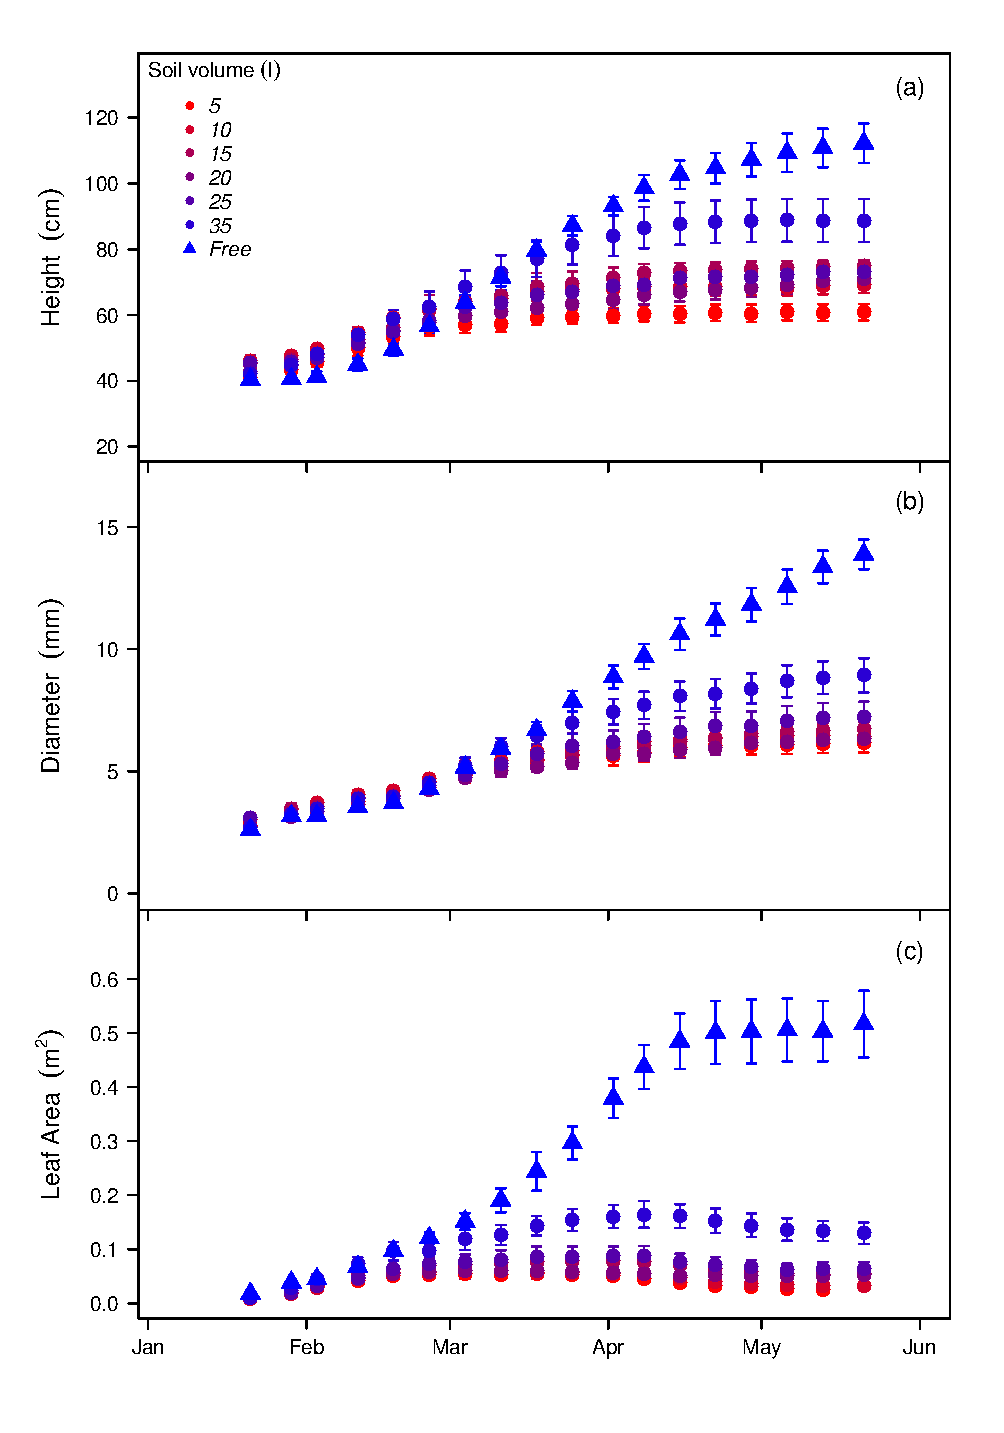
\includegraphics[width=0.99\textwidth]{allometry.pdf}
    \caption{Responses of plant and leaf characteristics of \textit{Eucalyptus tereticornis} seedlings to soil volume treatments. Each value reflects the mean(standard error) for each treatment. Seedling mass and leaf {\textdelta}\textsuperscript{13}C values are from final harvest. Values of leaf starch, sugars, nitrogen and SLA represent overall means across measurement campaigns (n=6). Different letters represent significant differences between treatments. The volume effect P value represents the overall difference between seedlings with soil volume restriction and the control seedlings.}
    \label{fig:figure 2.1}
\end{figure}

%figure 2.2
\begin{figure}[h!]
    \centering
    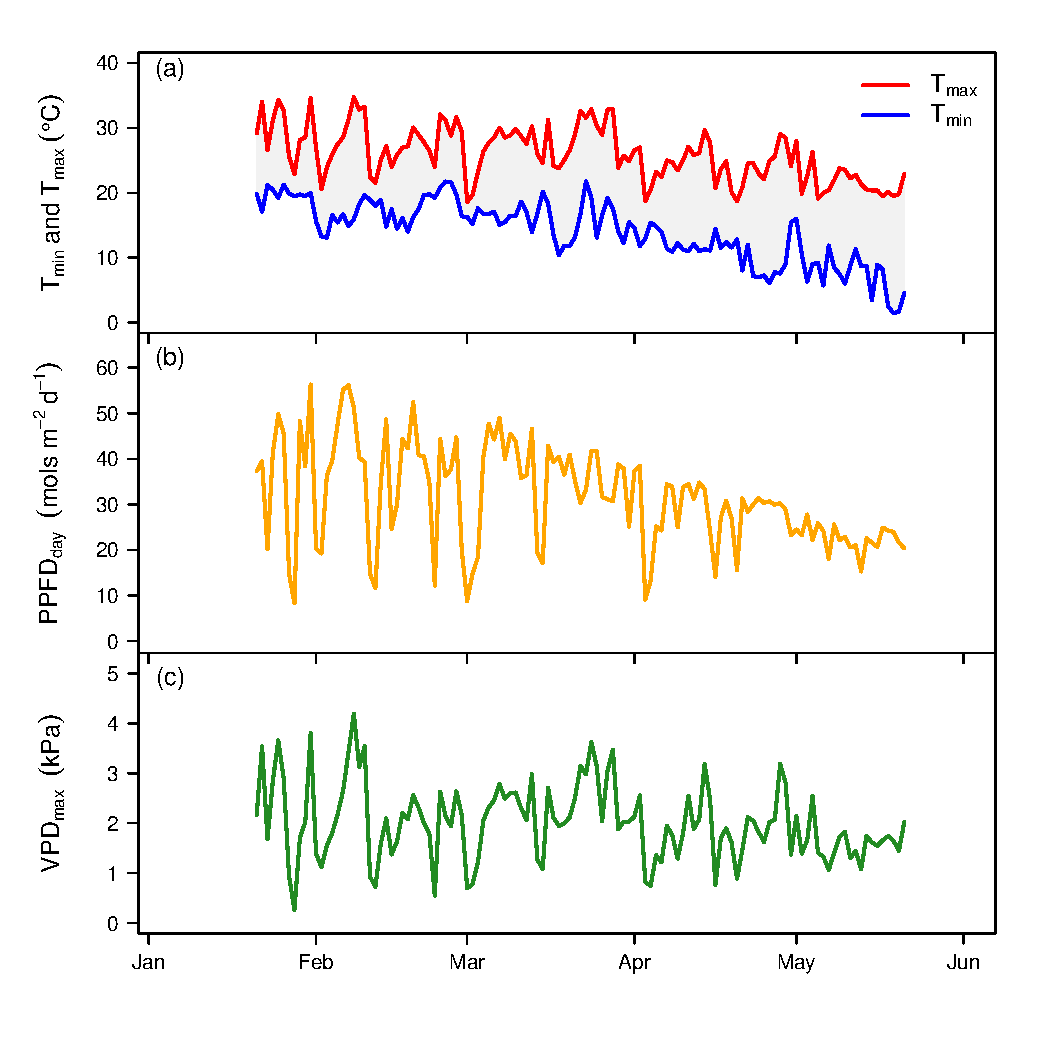
\includegraphics[width=0.99\textwidth]{airvars.pdf}
    \caption{Daily maximum and minimum temperature (a), total daily PPFD (b), and daily maximum vapour pressure deficit (c) across the experiment duration in 2013.}
    \label{fig:figure 2.2}
\end{figure}

%figure 2.3
\begin{figure}[h!]
    \centering
    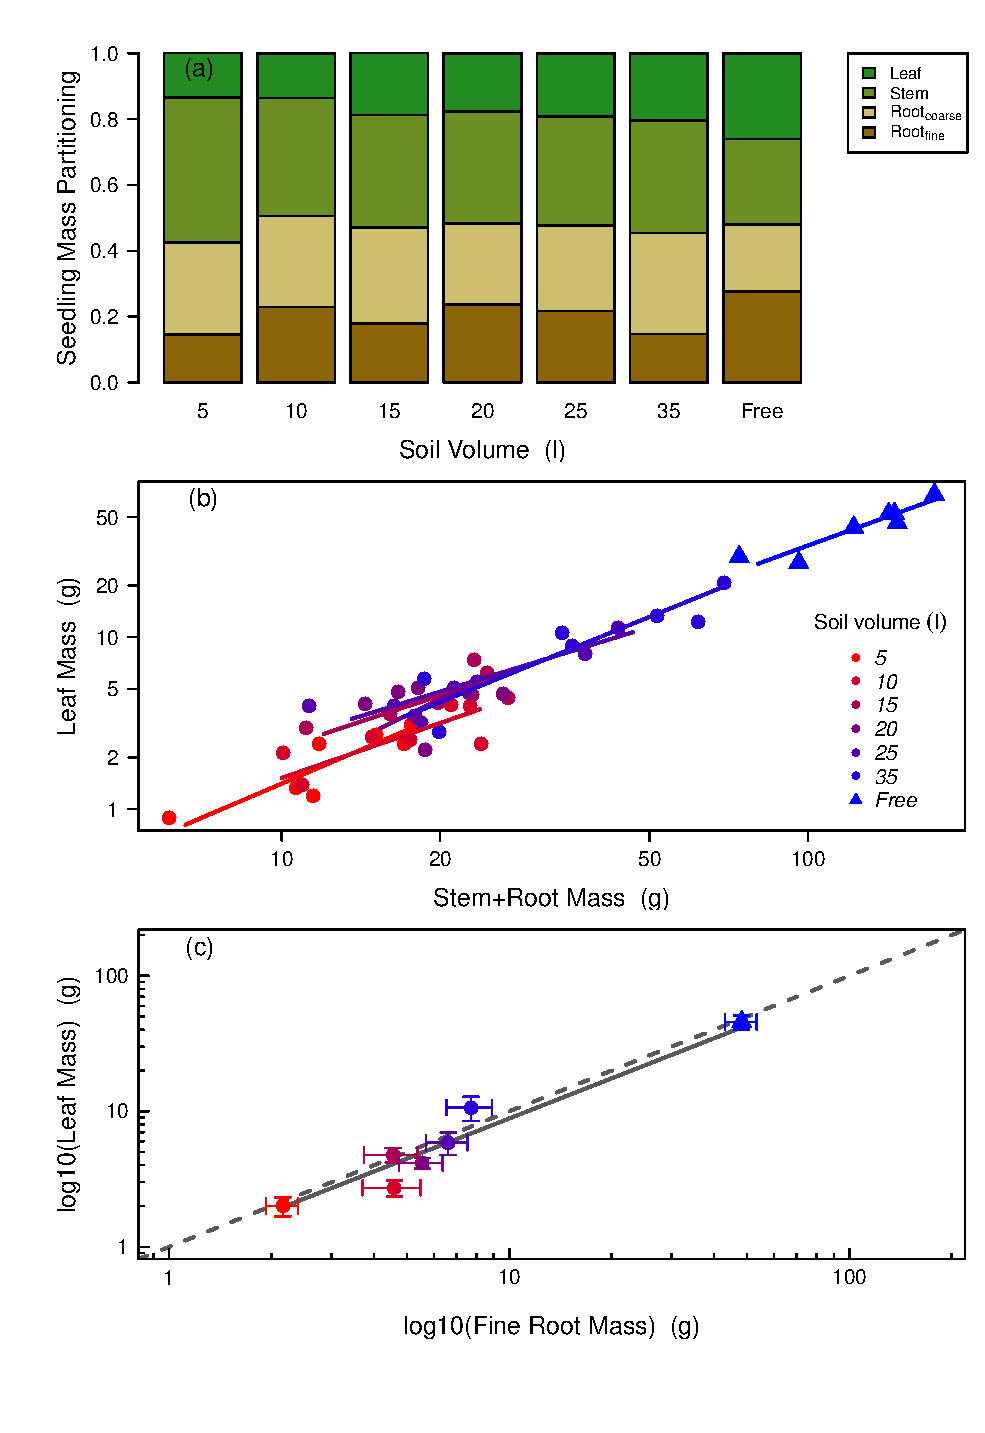
\includegraphics[width=0.99\textwidth]{massfractions.pdf}
    \caption{Soil volume treatment means of biomass partitioning to leaves, stems, and roots at harvest (a), bi-variate relationships between mass allocation to leaves and stems + roots (b) and leaf mass as a function of fine root biomass with $\pm$~standard error (c). For (b) lines represent standardized major axis fitting of the log-transformed allometric relationships of leaf mass fraction by treatment. For (c) the dashed line is the 1:1 relationship and the solid line represents the significant log-log model fit (R\textsuperscript{2} = 0.82) with equation: log(x) = 0.983(log(y)) - 0.036.}
    \label{fig:figure 2.3}
\end{figure}

%figure 2.4
\begin{figure}[h!]
    \centering
    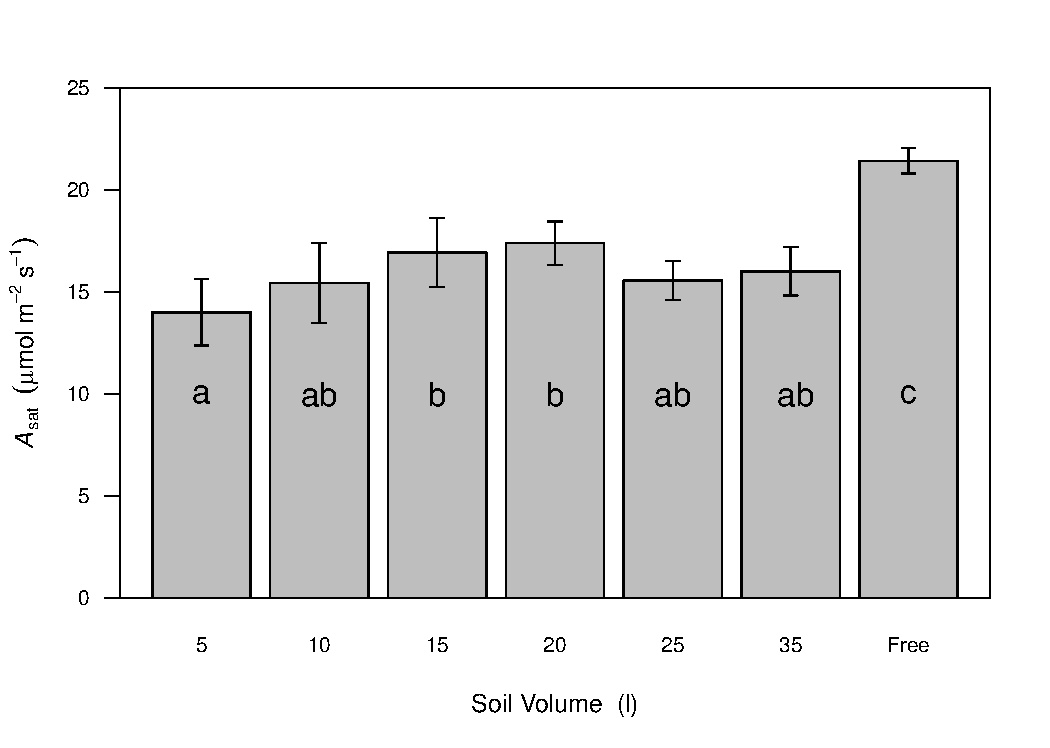
\includegraphics[width=0.99\textwidth]{Asat.pdf}
    \caption{Soil volume treatment means $\pm$~standard error, across all measurement campaigns (n = 6), of light saturated rates of photosynthesis at 25~$\degree$C. Different letters represent significant differences between treatments.}
    \label{fig:figure 2.4}
\end{figure}

%figure 2.5
\begin{figure}[h!]
    \centering
    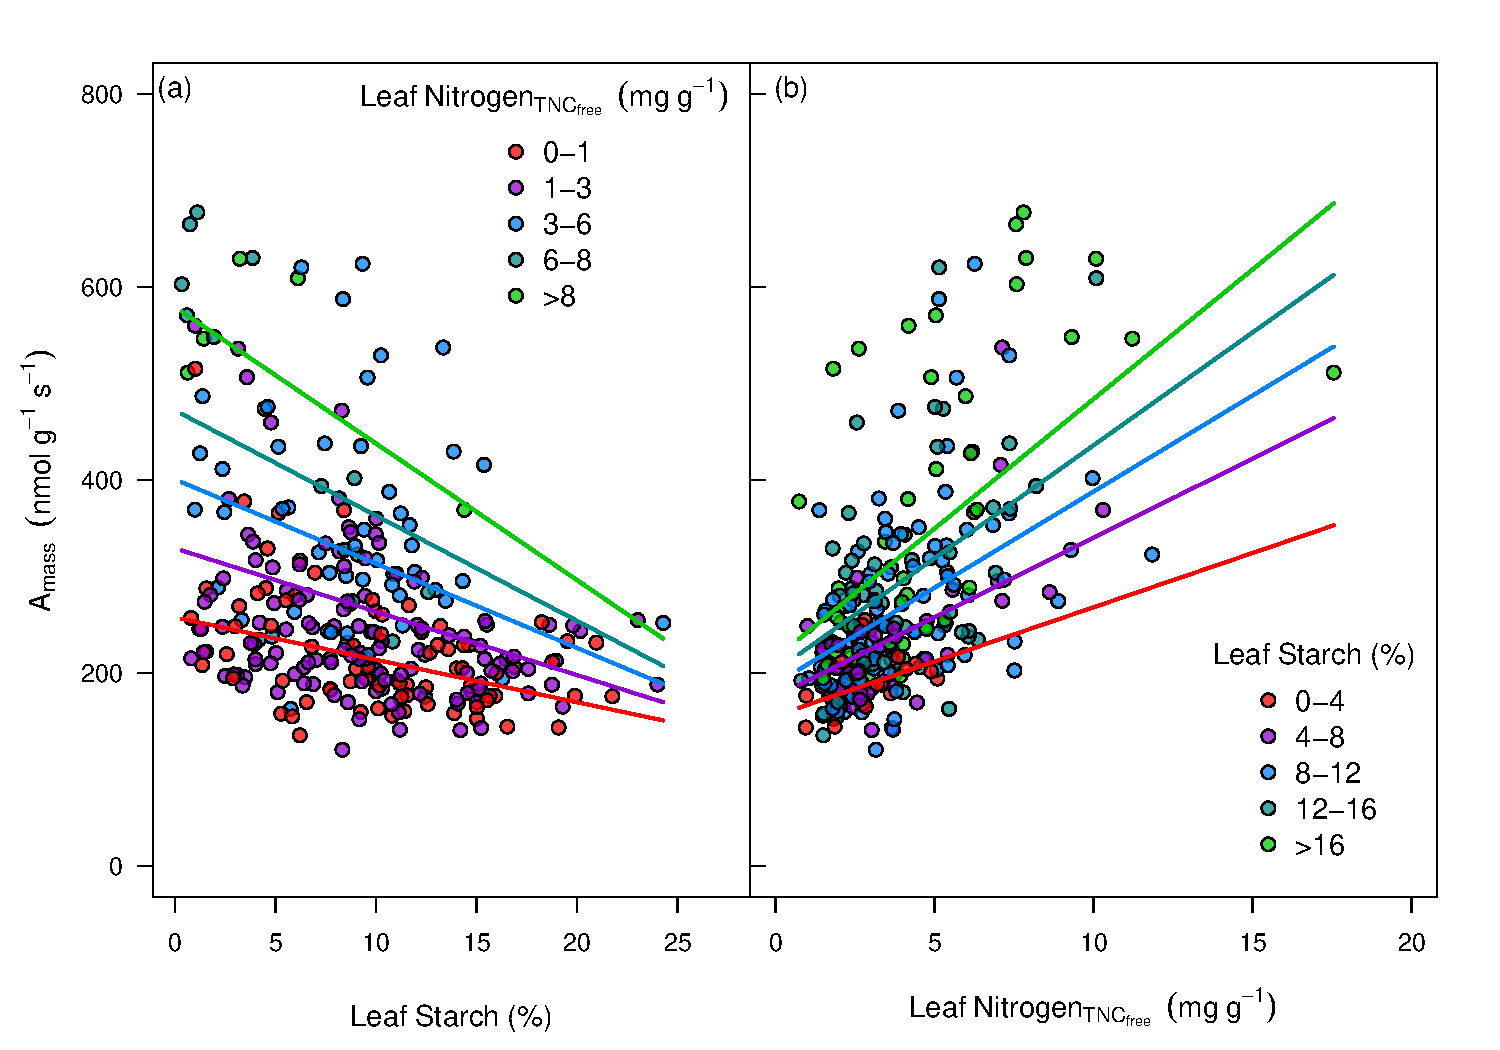
\includegraphics[width=0.99\textwidth]{A_leafchem.pdf}
    \caption{Photosynthetic capacity, on a leaf mass basis, as a function of accumulation of leaf starch (a) and leaf nitrogen content without TNC (b). Colors represent bins levels (n = 5) of both leaf starch and nitrogen grouped from low to high.  Lines represents predictions, for each bin level, from the linear mixed effects model equation of A\textsubscript{mass} as a function of starch and nitrogen. The marginal R\textsuperscript{2} (fixed effects only) was 0.37 and the conditional R\textsuperscript{2} (fixed and random effects) was 0.48 for the complete model.}
    \label{fig:figure 2.5}
\end{figure}

%figure 2.6
\begin{figure}[h!]
    \centering
    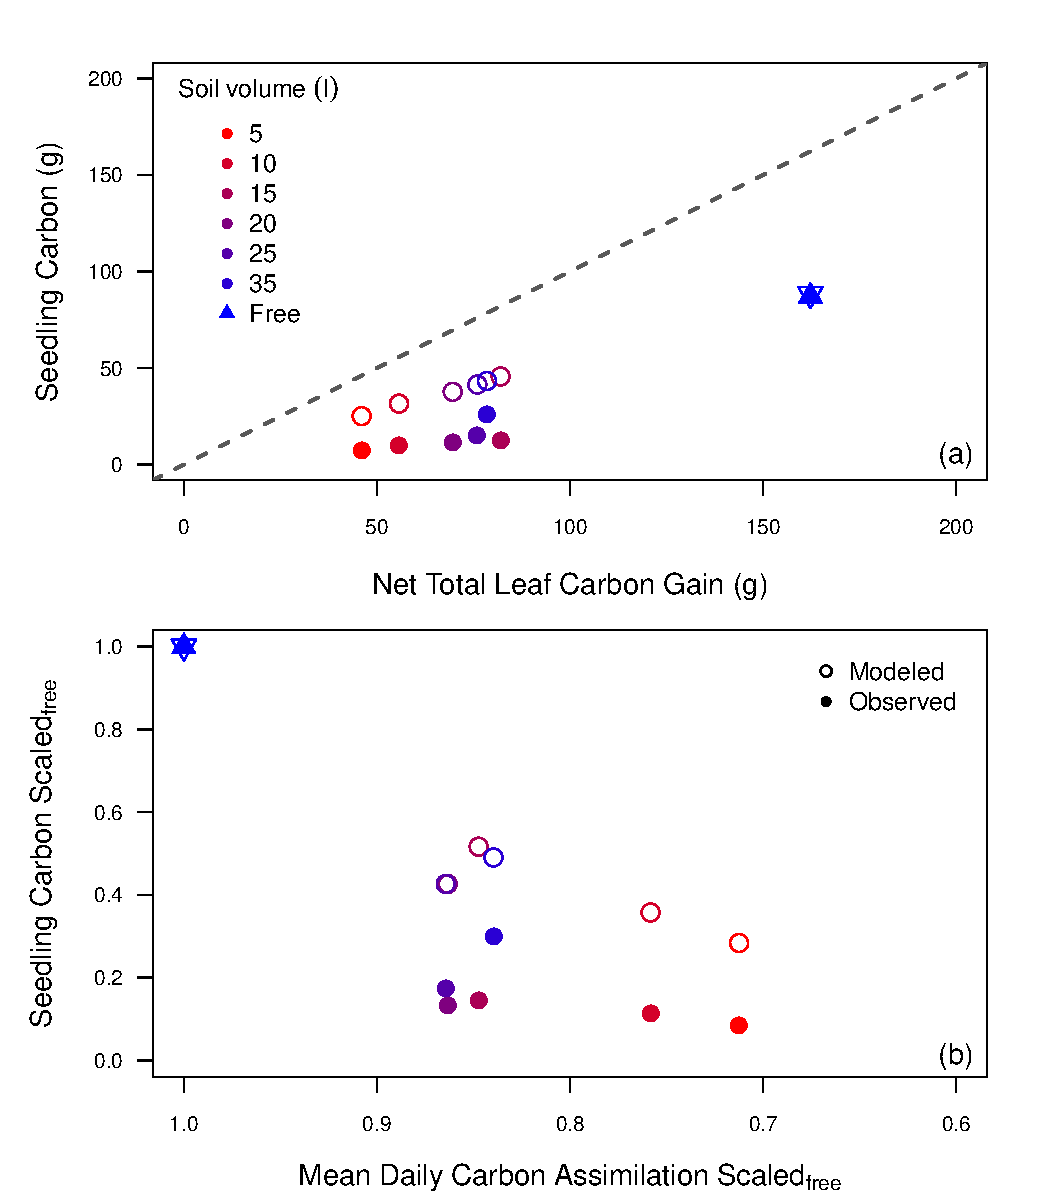
\includegraphics[width=0.99\textwidth]{massmodel_totalC.pdf}
    \caption{Total carbon mass for harvested and modeled seedlings versus predicted total carbon gain after 120 days (a) and  reductions in final seedling carbon mass, both modeled and observed, as a function of the reduction in leaf photosynthesis across treatments (b). For (a) the dashed 1:1 identifies the difference between net total leaf carbon gain and gross seedling production. For (b) both seedling carbon mass and daily carbon assimilation were first scaled to the free seedling control.}
    \label{fig:figure 2.6}
\end{figure}



%pvetable1
% latex table generated in R 3.2.3 by xtable 1.8-0 package
% Fri Dec 18 10:59:58 2015
\begin{sidewaystable}[ht]
\centering
\caption{Responses of plant and leaf characteristics of \textit{Eucalyptus tereticornis} seedlings to soil volume treatments. Each value reflects the mean($\pm$1 standard error) for each treatment. Seedling mass and leaf {\textdelta}\textsuperscript{13}C values are from final harvest. Values of leaf starch, sugars, nitrogen and SLA represent overall means across measurement campaigns (n=6). Different letters represent significant differences between treatments. The volume effect P value represents the overall difference between seedlings with soil volume restriction and the control seedlings.} 
\label{table:Table 2.1}
\begin{tabular}{lllllll}
  \hline
Volume (L) & Seedling~mass~(g) & SLA\textsubscript{TNC-free}~(m\textsuperscript{2}~kg\textsuperscript{-1}) & Leaf~Starch~(\%) & Leaf~Sugars~(\%) & Leaf~Nitrogen{TNC-free}~(\%) & {Leaf~\textdelta}\textsuperscript{13}C~(\text{\textperthousand}) \\ 
  \hline
5 & 14.8 (1.82) a & 11.8 (0.32) a & 12.7 (0.97) b & 6.4 (0.28) a & 1.3 (0.03) a & -30.1 (0.26) a \\ 
  10 & 20.0 (2.38) ab & 11.7 (0.31) a & 9.4 (0.75) ab & 6.7 (0.25) a & 1.5 (0.04) ab & -30.2 (0.25) a \\ 
  15 & 25.4 (2.49) ab & 12.7 (0.48) a & 7.3 (0.73) a & 7.2 (0.28) a & 1.6 (0.07) ab & -30.3 (0.36) a \\ 
  20 & 23.4 (1.63) ab & 11.8 (0.37) a & 9.5 (0.88) ab & 6.6 (0.26) a & 1.7 (0.06) ab & -29.7 (0.28) a \\ 
  25 & 30.4 (5.49) ab & 12.4 (0.40) a & 9.8 (0.71) ab & 6.9 (0.24) a & 1.6 (0.07) ab & -29.7 (0.25) a \\ 
  35 & 52.2 (9.55) b & 13.5 (0.46) ab & 9.8 (0.65) ab & 6.8 (0.22) a & 1.8 (0.08) b & -30.6 (0.38) a \\ 
  Free & 174.5 (18.02) c & 15.1 (0.47) b & 6.8 (0.65) a & 7.4 (0.25) a & 2.7 (0.09) c & -30.0 (0.34) a \\ 
   \hline
Volume Effect (P value) & 0.001 & 0.001 & 0.029 & 0.125 & 0.001 & 0.372 \\ 
   \hline
\end{tabular}
\end{sidewaystable}




%pvetable2
% latex table generated in R 3.2.3 by xtable 1.8-0 package
% Fri Dec 18 10:59:59 2015
\begin{sidewaystable}[ht]
\centering
\caption{Responses of root characteristics of \textit{Eucalyptus tereticornis} seedlings to soil volume treatments. Each value reflects the mean ($\pm$1 standard error) for each treatment. All values are from the final harvest. Values for FRLD were only calculated for seedlings in containers as free seedlings had potentially unlimited soil volume to exploit. Different letters represent significant differences between treatments. The volume effect P value represents the overall difference between seedlings with soil volume restriction and the control seedlings, except for FRLD which represents only differences between seedlings in containers.} 
\label{table:Table 2.2}
\begin{tabular}{llll}
  \hline
Root~Nitrogen~(\%) & SRL~(cm~m\textsuperscript{-1}) & FRLD~(m~dm\textsuperscript{-3}) & NA \\ 
  \hline
5 & 0.78 (0.04) ab & 73.0 (6.73) ab & 36.4 (5.68) bc \\ 
  10 & 0.75 (0.02) a & 99.6 (8.70) b & 45.9 (8.68) c \\ 
  15 & 0.71 (0.02) a & 74.6 (6.98) ab & 20.9 (1.51) ab \\ 
  20 & 0.76 (0.04) a & 85.8 (7.37) ab & 23.0 (3.09) ab \\ 
  25 & 0.74 (0.02) a & 82.5 (15.02) ab & 24.7 (7.58) ab \\ 
  35 & 0.77 (0.03) ab & 63.1 (6.47) a & 13.3 (1.98) a \\ 
  Free & 0.90 (0.03) b & 50.9 (5.00) a &  \\ 
   \hline
Volume Effect (P value) & 0.017 & 0.009 & 0.001 \\ 
   \hline
\end{tabular}
\end{sidewaystable}



%pvetable3
% latex table generated in R 3.2.3 by xtable 1.8-0 package
% Fri Dec 18 10:59:59 2015
\begin{sidewaystable}[ht]
\centering
\caption{Responses of leaf level gas exchange parameters of \textit{Eucalyptus tereticornis} seedlings to soil volume treatments. Each value reflects the mean ($\pm$1 standard error) for each treatment. \textit{A}\textsubscript{max}, \textit{R}\textsubscript{dark} and \textit{g}\textsubscript{s} are each measured at 25$\degree$C. Values of \textit{A}\textsubscript{max}, \textit{g}\textsubscript{s} and \textit{g}\textsubscript{1} represent overall means across measurement campaigns (n=6). \textit{R}\textsubscript{dark}, \textit{J}\textsubscript{max} and \textit{Vc}\textsubscript{max} values are means of two measurement campaigns at beginning and end of gas exchange measurements. Different letters represent significant differences between treatments. The volume effect P value represents the overall difference between seedlings with soil volume restriction and the control seedlings.} 
\label{table:Table 2.3}
\begin{tabular}{lllllll}
  \hline
Volume~(L) & \textit{A}\textsubscript{max}~({\textmugreek}mol~m\textsuperscript{-2}~s\textsuperscript{-1}) & \textit{R}\textsubscript{dark}~({\textmugreek}mol~m\textsuperscript{-2}~s\textsuperscript{-1}) & \textit{J}\textsubscript{max} & \textit{Vc}\textsubscript{max} & \textit{g}\textsubscript{s}~(mol~m\textsuperscript{-1}~s\textsuperscript{-1}) & \textit{g}\textsubscript{1} \\ 
  \hline
5 & 21.2 (0.9) a & 0.61 (0.04) a & 104.5 (3.3) a & 63.3 (2.5) a & 0.30 (0.009) a & 5.1 (0.14) bc \\ 
  10 & 22.3 (1.4) ab & 0.79 (0.06) a & 116.5 (7.5) a & 69.4 (4.7) a & 0.36 (0.009) ab & 5.4 (0.10) cd \\ 
  15 & 23.3 (1.2) ab & 0.70 (0.05) a & 125.4 (7.8) a & 80.8 (5.1) ab & 0.42 (0.010) ab & 5.8 (0.14) d \\ 
  20 & 26.1 (0.7) b & 0.73 (0.11) a & 131.5 (8.6) a & 82.1 (4.7) ab & 0.37 (0.011) ab & 4.9 (0.12) ac \\ 
  25 & 23.9 (0.9) ab & 0.53 (0.13) a & 132.8 (13.1) a & 79.0 (8.7) a & 0.30 (0.009) a & 4.5 (0.14) a \\ 
  35 & 25.0 (1.0) ab & 0.61 (0.04) a & 127.2 (6.1) a & 82.4 (3.6) a & 0.31 (0.011) a & 4.4 (0.15) a \\ 
  Free & 33.1 (0.7) c & 0.64 (0.07) a & 169.0 (8.2) b & 100.4 (3.3) b & 0.44 (0.011) b & 4.5 (0.14) ab \\ 
   \hline
Volume Effect (P value) & 0.001 & 0.269 & 0.004 & 0.005 & 0.007 & 0.001 \\ 
   \hline
\end{tabular}
\end{sidewaystable}



\subsection*{DISCUSSION}
\subsection*{SUPPORTING INFORMATION}


%modtable
% latex table generated in R 3.2.3 by xtable 1.8-0 package
% Fri Dec 18 10:59:59 2015
\begin{sidewaystable}[ht]
\centering
\caption{Seedling growth model default parameters.} 
\label{table:Table 2.S1}
\begin{tabular}{lllll}
  \hline
Variable & Description & Default.Value & Units & Source \\ 
  \hline
Leaf area$\backslash$textsubscript\{i\} & initial leaf area & 0.035 & m\verb|^|2\verb|^| & this study \\ 
  Leaf mass$\backslash$textsubscript\{i\} & initial leaf mass & 3.45 & g & this study \\ 
  Stem mass$\backslash$textsubscript\{i\} & initial stem mass & 1.51 & g & this study \\ 
  Root mass$\backslash$textsubscript\{i\} & initial root mass & 0.99 & g & this study \\ 
  $\backslash$epsilon$\backslash$textsubscript\{c\} & biomass conversion efficiency & 0.65 & g C g mass\verb|^|-1\verb|^| & M?kel? (1997) \\ 
  R$\backslash$textsubscript\{coarse\}\~{}$\backslash$textsubscript\{root\} & coarse root respiration & 0.00124 & g C g root\verb|^|-1\verb|^| d\verb|^|-1\verb|^| & Marden et al. (2008) \\ 
  R$\backslash$textsubscript\{fine\}\~{}$\backslash$textsubscript\{root\} & fine root respiration & 0.01037 & g C g root\verb|^|-1\verb|^| d\verb|^|-1\verb|^| & Ryan et al. (2010) \\ 
   \hline
R$\backslash$textsubscript\{stem\} & stem respiration & 0.00187 & g C g stem\verb|^|-1\verb|^| d\verb|^|-1\verb|^| & Drake et al. (unpublished) \\ 
  C$\backslash$textsubscript\{day\} & daily leaf carbon assimilation & 5.4 - 7.6 & g C m\verb|^|-2\verb|^| d\verb|^|-1\verb|^| & this study \\ 
  $\backslash$Lambda & leaf or root turnover & 1 & yr\verb|^|-1\verb|^| & theoretical \\ 
   \hline
\end{tabular}
\end{sidewaystable}


%figure 2.S1
\begin{figure}[h!]
    \centering
    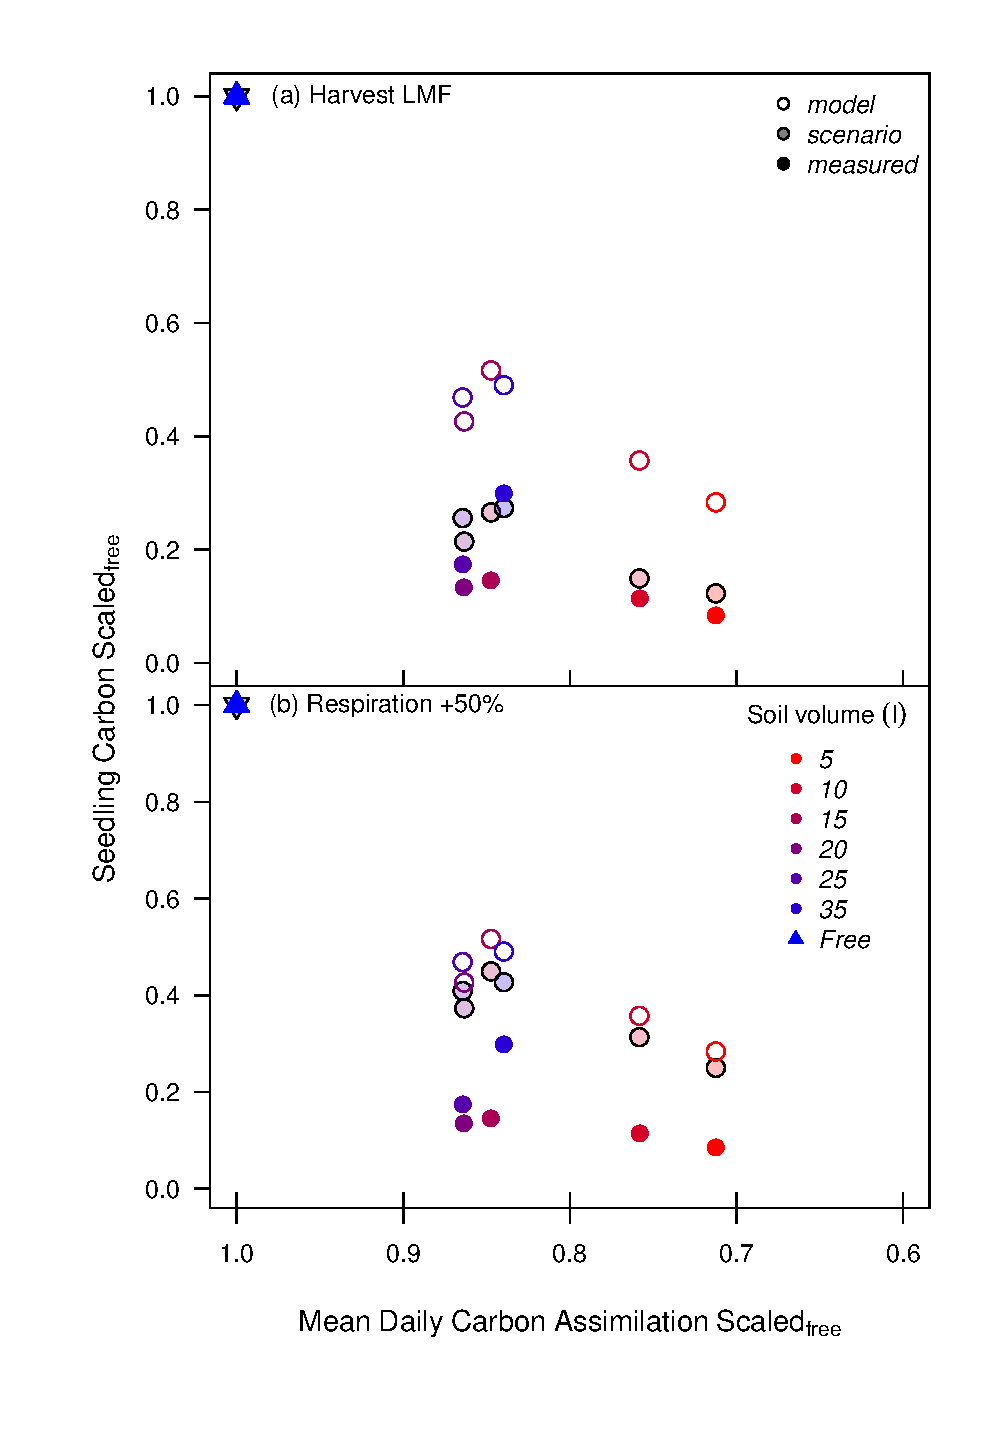
\includegraphics[width=0.99\textwidth]{massmodel_resp.pdf}
    \caption{Sensitivity testing of seedling growth model to different carbon allocation strategies including; constraints of leaf mass fraction to treatment specific final harvest values (a) and increases in respiration of non-leaf tissue components by 50~\% (b). Open and filled symbols represent default model and harvest values, while shaded symbols represent model sensitivity to each scenario by soil volume treatment. Both seedling carbon mass and daily carbon assimilation were first scaled to the free seedling control.}
    \label{fig:figure 2.S1}
\end{figure}

   
\addcontentsline{toc}{section}{CHAPTER 2 BELOWGROUND SINK LIMITATION ALTERS GROWTH AND CARBON BALANCE OF EUCALYPTUS SEEDLINGS}
\addcontentsline{toc}{subsection}{ABSTRACT}
\addcontentsline{toc}{subsection}{INTRODUCTION}
\addcontentsline{toc}{subsection}{MATERIALS AND METHODS}
\addcontentsline{toc}{subsection}{RESULTSS}
\addcontentsline{toc}{subsection}{DISCUSSION}
\addcontentsline{toc}{subsection}{SUPPORTING INFORMATION}
\clearpage
%--------------------------------------------------------------------------------------------%

% Load data for tables chapter 3



\section*{CHAPTER 3 \\ \mbox{ }\\ Rapid response of mesophyll conductance to light availability allows shade leaves to take advantage of sunflecks}
\subsection*{ABSTRACT}
\subsection*{INTRODUCTION}
\subsection*{MATERIALS AND METHODS}
\subsection*{RESULTS}

%figure 3.1
\begin{figure}[h!]
    \centering
    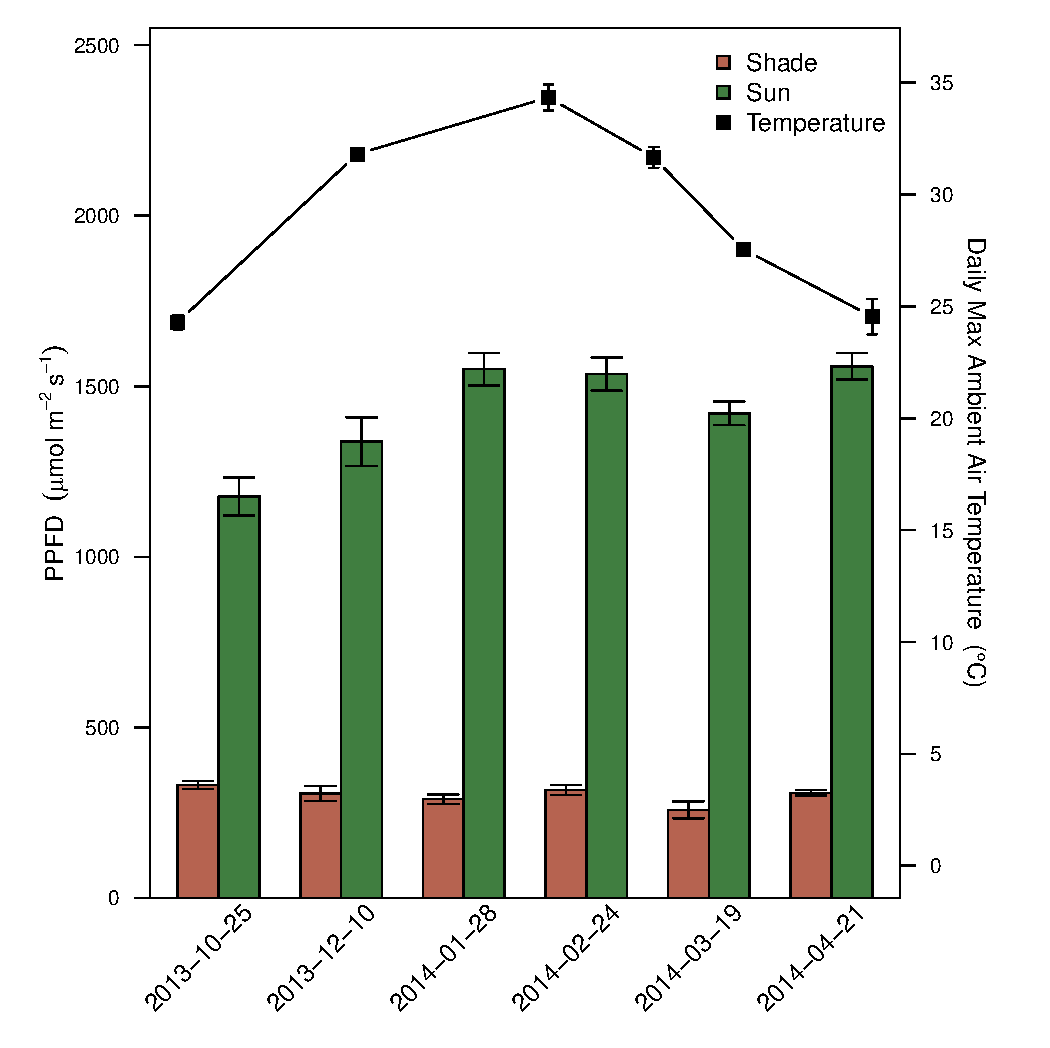
\includegraphics[width=0.99\textwidth]{ppfd2.pdf}
    \caption{Bars represent the local light environment for sun and shade leaves during six gas exchange campaigns from October 2013 to April 2014. Means $\pm$~1 standard error represent integrated PPFD, measured with a ceptometer, at the canopy height of each selected leaf. Each date represents the starting date for each measurement campaign. Points represent the mean ($\pm$~1 standard error) daily maximum air temperature during each campaign period.}
    \label{fig:figure 3.1}
\end{figure}


%wtc1tab
% latex table generated in R 3.2.3 by xtable 1.8-0 package
% Fri Dec 18 10:59:59 2015
\begin{sidewaystable}[ht]
\centering
\caption{\textit{Eucalyptus tereticornis} leaf morphological and physiological traits between full sun and shade leaves under ambient and elevated temperature treatments. Leaf mass per area, N	extsubscript{a}, {\textdelta}\textsuperscript{13}C, $\Psi\textsubscript{pd}$, $\Psi\textsubscript{l}$ and K	extsubscript{l} values represent treatment mean ($\pm$~1~standard error) across measurement campaigns (n=6). Values of Vc\textsubscript{max} and J\textsubscript{max} are treatment mean ($\pm$ 1 standard error) from AC\textsubscript{i} curves measured in each chamber at saturating light. Units of LMA and Leaf N\textsubscript{area} are g~m\textsuperscript{2}, K\textsubscript{l} is mmol~m\textsuperscript{-2}~s\textsuperscript{-1} MPa, WP is MPA and {\textdelta}\textsuperscript{13}C is \permil. Different letters represent significant differences between leaf type and temperature treatments. The P value represents the overall effect between each unique combination of leaf type and temperature treatment for each trait.} 
\label{table:Table 3.1}
\begin{tabular}{llllllllll}
  \hline
Leaf & Temperature & LMA & N\textsubscript{a} & Vc\textsubscript{max} & J\textsubscript{max} & K & WP\textsubscript{pre} & WP\textsubscript{mid} & {\textdelta}\textsuperscript{13}C \\ 
  \hline
Sun & AT & 114.1 (4.5) a & 2.63 (0.08) b & 96.0 (6.7) b & 141.6 (7.5) b & 1.69 (0.18) a & -0.32 (0.03) a & -1.60 (0.10) a & -28.1 (0.18) b \\ 
   & ET & 109.9 (4.8) a & 2.60 (0.09) b & 95.5 (6.6) ab & 148.3 (11.8) b & 1.79 (0.15) a & -0.32 (0.02) a & -1.70 (0.09) a & -28.3 (0.17) b \\ 
  Shade & AT & 118.3 (4.4) a & 2.13 (0.07) a & 73.3 (6.4) a & 102.1 (6.9) a & 1.70 (0.13) a & -0.27 (0.02) a & -1.50 (0.09) a & -29.9 (0.17) a \\ 
   & ET & 113.1 (4.3) a & 1.88 (0.06) a & 77.6 (4.9) ab & 106.2 (6.5) a & 1.78 (0.14) a & -0.30 (0.02) a & -1.60 (0.11) a & -30.4 (0.22) a \\ 
   \hline
P value &  & 0.785 & 0.001 & 0.028 & 0.002 & 0.001 & 0.3486 & 0.6385 & 0.973 \\ 
   \hline
\end{tabular}
\end{sidewaystable}



%figure 3.2
\begin{figure}[h!]
    \centering
    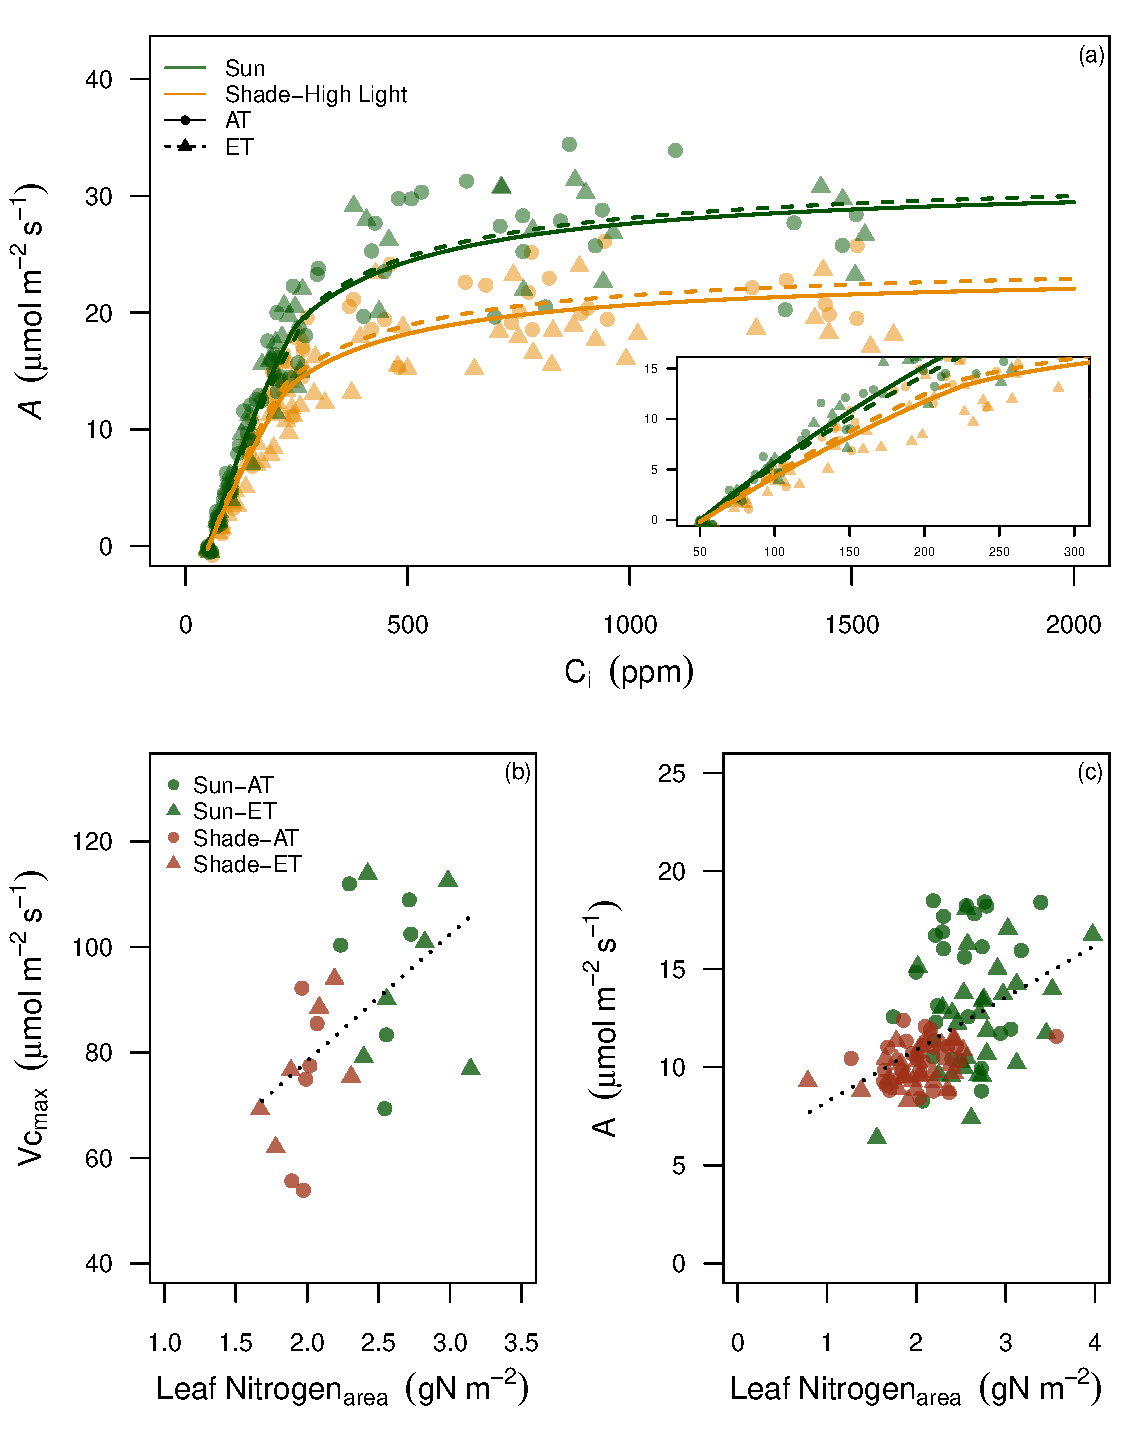
\includegraphics[width=0.99\textwidth]{aci_nitrovcmax.pdf}
    \caption{(a) AC\textsubscript{i} curves for sun and shade leaves at elevated (ET) and ambient (AT) temperature treatments. AC\textsubscript{i} curves were measured once on all trees, in February 2014, at 25~$\degree$C and at saturating light (1800~{\textmugreek}mol~m\textsuperscript{-1}~s\textsuperscript{-1}). (b) The relationship between Vc\textsubscript{max} and mean leaf N\textsubscript{a} for each chamber, including sun leaves and shade leaves at low light. (c) The relationship between A\textsubscript{n} and leaf N\textsubscript{a} for sun and shade leaves measured under their ambient light and temperature conditions. For (b,c) the dashed line represents the significant linear model fit for all leaves, with a marginal and conditional R\textsuperscript{2} of 0.28 and 0.35 for (b) and 0.24 and 0.33 for (c).}
    \label{fig:figure 3.2}
\end{figure}

%wtc1tab
% latex table generated in R 3.2.3 by xtable 1.8-0 package
% Fri Dec 18 10:59:59 2015
\begin{sidewaystable}[ht]
\centering
\caption{Responses of \textit{Eucalyptus tereticornis} leaf gas exchange parameters for sun and shade leaves under ambient and elevated temperature treatments. Each value reflects the mean ($\pm$~1~standard error) for each treatment across gas exchange campaigns (n=6). Units for A and E are {\textmugreek}mol~m\textsuperscript{-2}~s\textsuperscript{-1}, for g\textsubscript{s} and g\textsubscript{m} are mol~m\textsuperscript{-2}~s\textsuperscript{-1} and for VPD are kPa. Different letters represent significant differences between leaf type, light environment and temperature treatments. The P value represents the overall effect between each unique combination of leaf type, light environment and temperature treatment for each parameter.} 
\label{table:Table 3.2}
\begin{tabular}{lllllllllll}
  \hline
Leaf & Light & Temperature & A & g\textsubscript{s} & g\textsubscript{m} & ITE & E & VPD & C\textsubscript{i} & C\textsubscript{c} \\ 
  \hline
Sun & High & AT & 13.5 (0.3) b & 0.122 (0.005) a & 0.163 (0.005) c & 8.26 (0.48) b & 1.78 (0.07) a & 1.60 (0.04) ab & 179.8 ( 3.2) a & 92.2 ( 2.9) a \\ 
   &  & ET & 13.1 (0.3) b & 0.123 (0.005) a & 0.153 (0.007) bc & 6.57 (0.39) ab & 2.21 (0.09) a & 1.90 (0.05) b & 187.9 ( 2.9) a & 92.2 ( 2.8) a \\ 
  Shade & Low & AT & 10.4 (0.1) a & 0.150 (0.005) a & 0.117 (0.004) ab & 6.24 (0.50) a & 1.93 (0.07) a & 1.40 (0.04) a & 255.4 ( 3.8) b & 160.0 ( 4.1) c \\ 
   &  & ET & 10.0 (0.1) a & 0.146 (0.005) a & 0.116 (0.004) a & 5.43 (0.51) a & 2.23 (0.09) a & 1.60 (0.05) a & 253.8 ( 4.1) b & 160.3 ( 3.5) bc \\ 
   & High & AT & 18.1 (0.3) c & 0.255 (0.007) b & 0.184 (0.003) c & 5.85 (0.33) a & 3.42 (0.12) b & 1.40 (0.04) a & 237.4 ( 2.2) b & 137.4 ( 1.9) b \\ 
   &  & ET & 16.7 (0.2) c & 0.246 (0.009) b & 0.177 (0.003) c & 5.02 (0.35) a & 3.81 (0.15) b & 1.70 (0.04) ab & 238.1 ( 3.2) b & 141.7 ( 2.8) bc \\ 
   \hline
P value &  &  & 0.001 & 0.001 & 0.001 & 0.001 & 0.001 & 0.005 & 0.001 & 0.001 \\ 
   \hline
\end{tabular}
\end{sidewaystable}



%figure 3.3
\begin{figure}[h!]
    \centering
    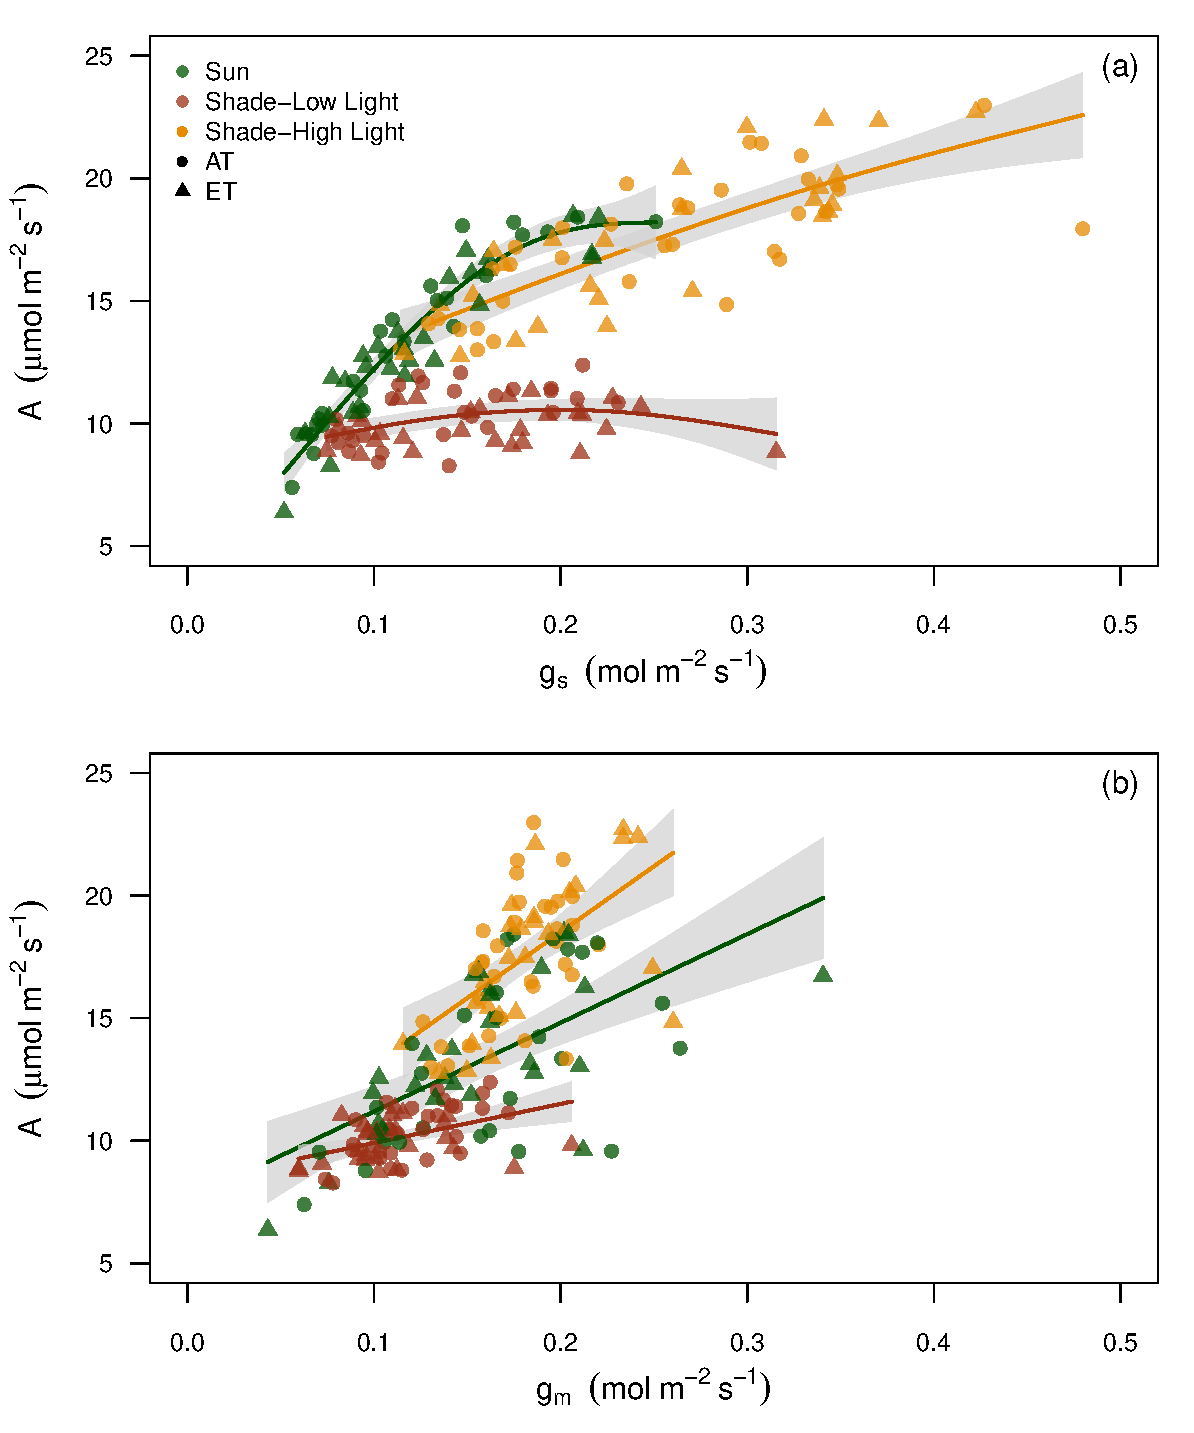
\includegraphics[width=0.99\textwidth]{Agmgs.pdf}
    \caption{The response of A to g\textsubscript{s} (a) and g\textsubscript{m} (b) for sun leaves measured at high light and shade leaves measured at both low and high light under their respective elevated and ambient temperature treatments. Lines represent either smoothed regressions from a generalized additive model fit (a) or linear model fits (b). Grey areas are 95\% confidence intervals from the mean.}
    \label{fig:figure 3.3}
\end{figure}

%figure 3.4
\begin{figure}[h!]
    \centering
    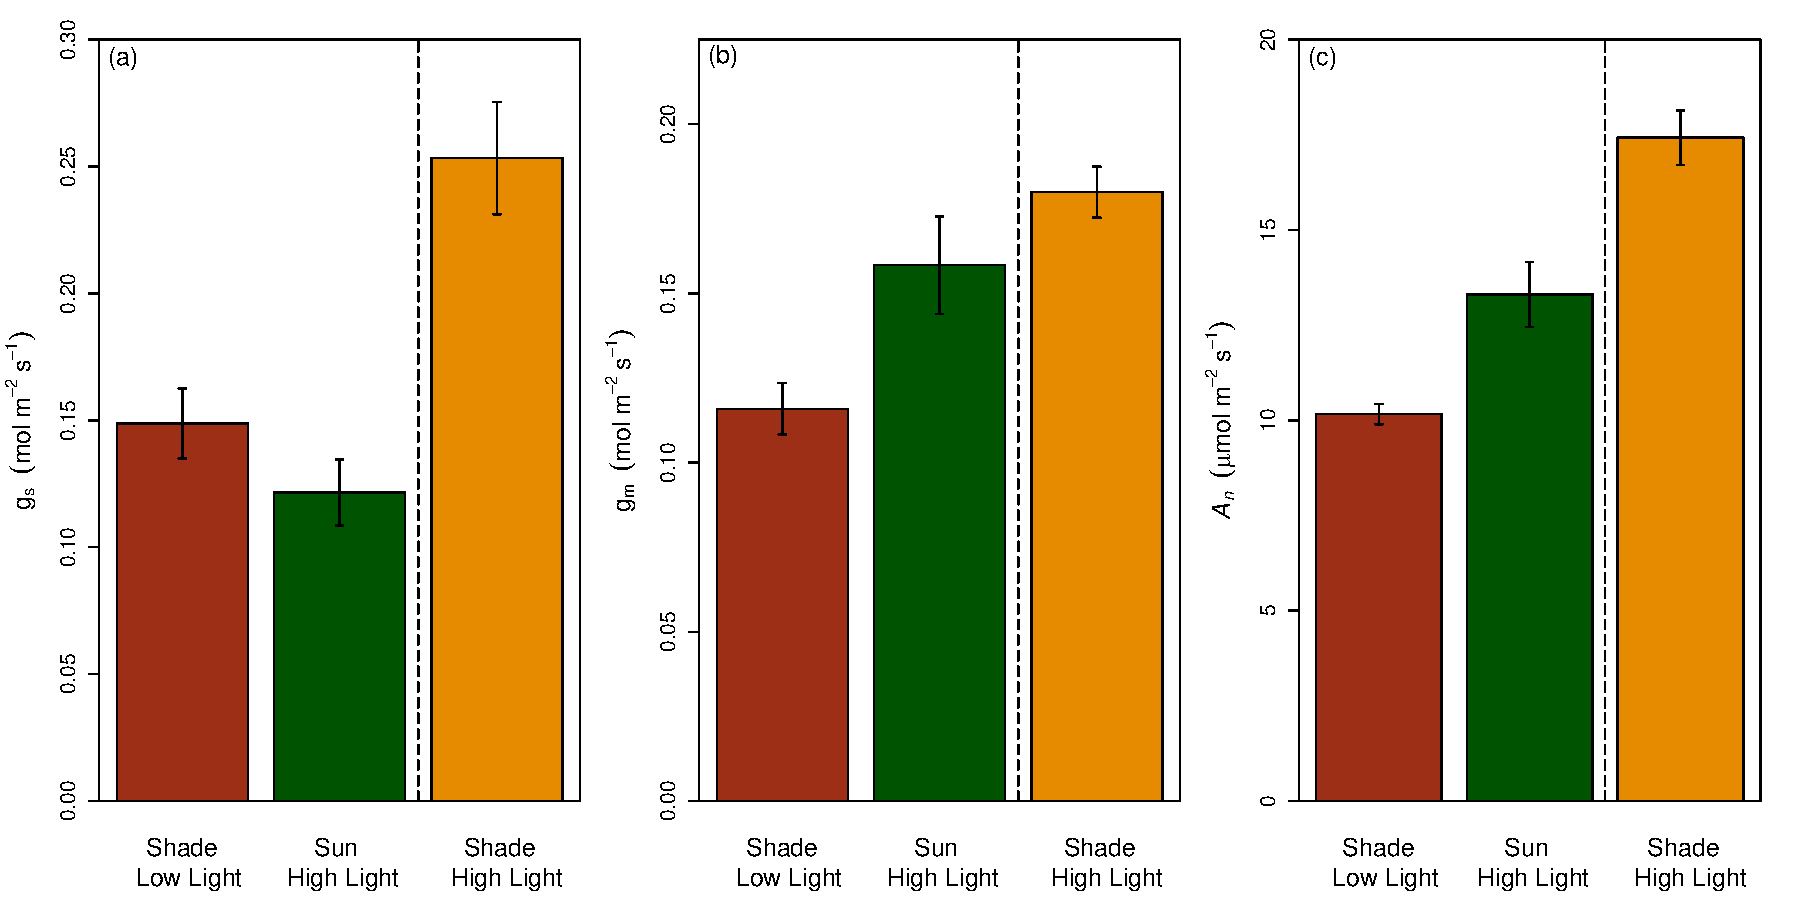
\includegraphics[width=0.99\textwidth]{physiology_bar.pdf}
    \caption{The mean $\pm$~1 standard error of g\textsubscript{s} (a), g~\textsubscript{m} (b) and A\textsubscript{n} (c) of sun leaves and shade leaves at both low and high light pooled across six measurement dates.}
    \label{fig:figure 3.4}
\end{figure}

%figure 3.5
\begin{figure}[h!]
    \centering
    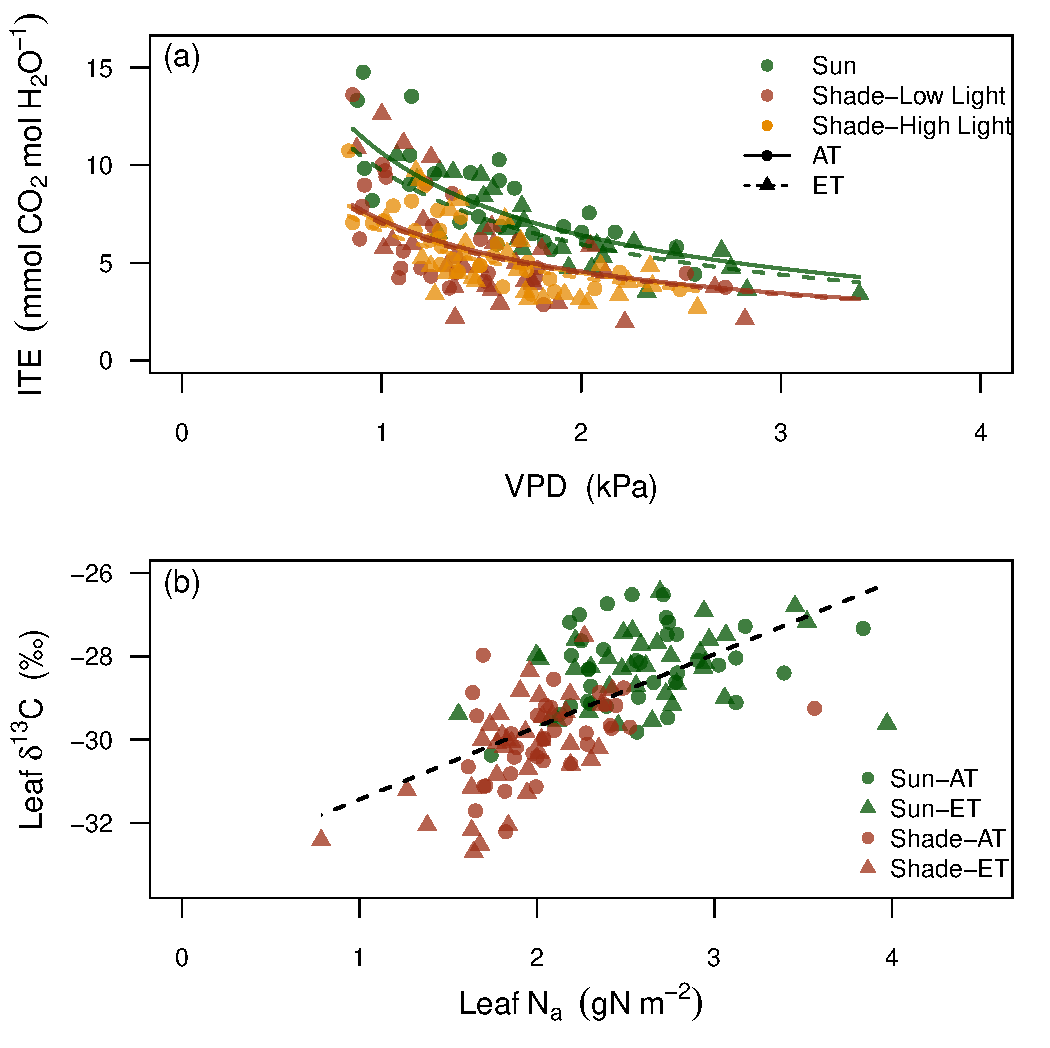
\includegraphics[width=0.99\textwidth]{ITE_13c.pdf}
    \caption{(a) Response of instantaneous transpiration efficiency (ITE) to VPD for sun leaves and shade leaves at both low and high light with elevated and ambient temperature treatments. (b) The relationship between leaf {\textdelta}\textsuperscript{13}C and leaf N\textsubscript{a} for sun leaves at high light and shade leaves at low light. For (a) VPD is the leaf to air pressure difference inside the gas exchange cuvette and lines represent predictions from the optimal ITE model with a g\textsubscript{1} value for each leaf type and treatment. For (b) the dashed line represents the significant linear model fit for all leaves with a marginal and conditional R\textsuperscript{2}~=~ of 0.41 and 0.45, respectively.}
    \label{fig:figure 3.5}
\end{figure}

%figure 3.6
\begin{figure}[h!]
    \centering
    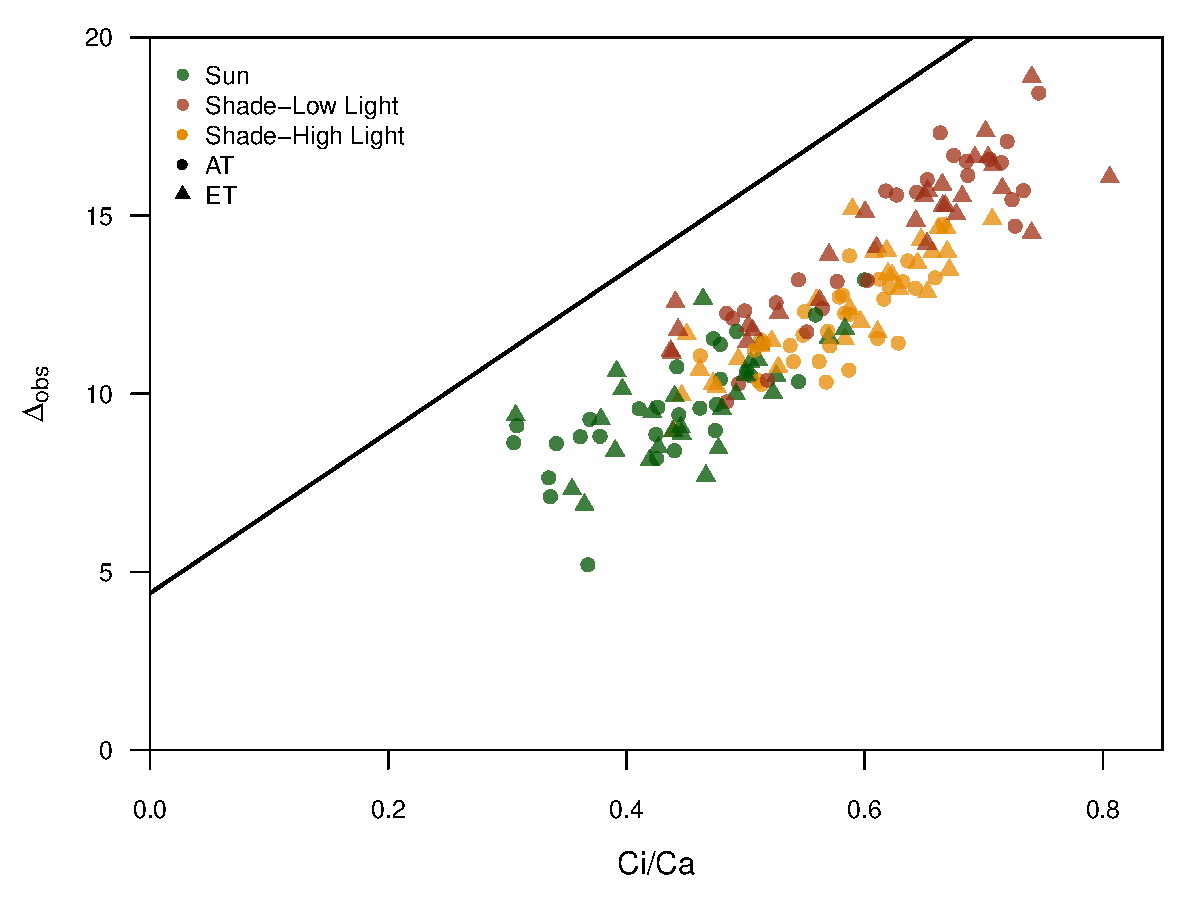
\includegraphics[width=0.99\textwidth]{delta_cica.pdf}
    \caption{Relationship between the observed discrimination of \textsuperscript{13}CO\textsubscript{2} measured during photosynthesis and measured C\textsubscript{i}/C\textsubscript{a} for sun leaves measured at high light and shade leaves measured at both low and high light. The solid line represents the theoretical line for C3 plants from \citet{evans1986carbon}.}
    \label{fig:figure 3.6}
\end{figure}

%figure 3.7
\begin{figure}[h!]
    \centering
    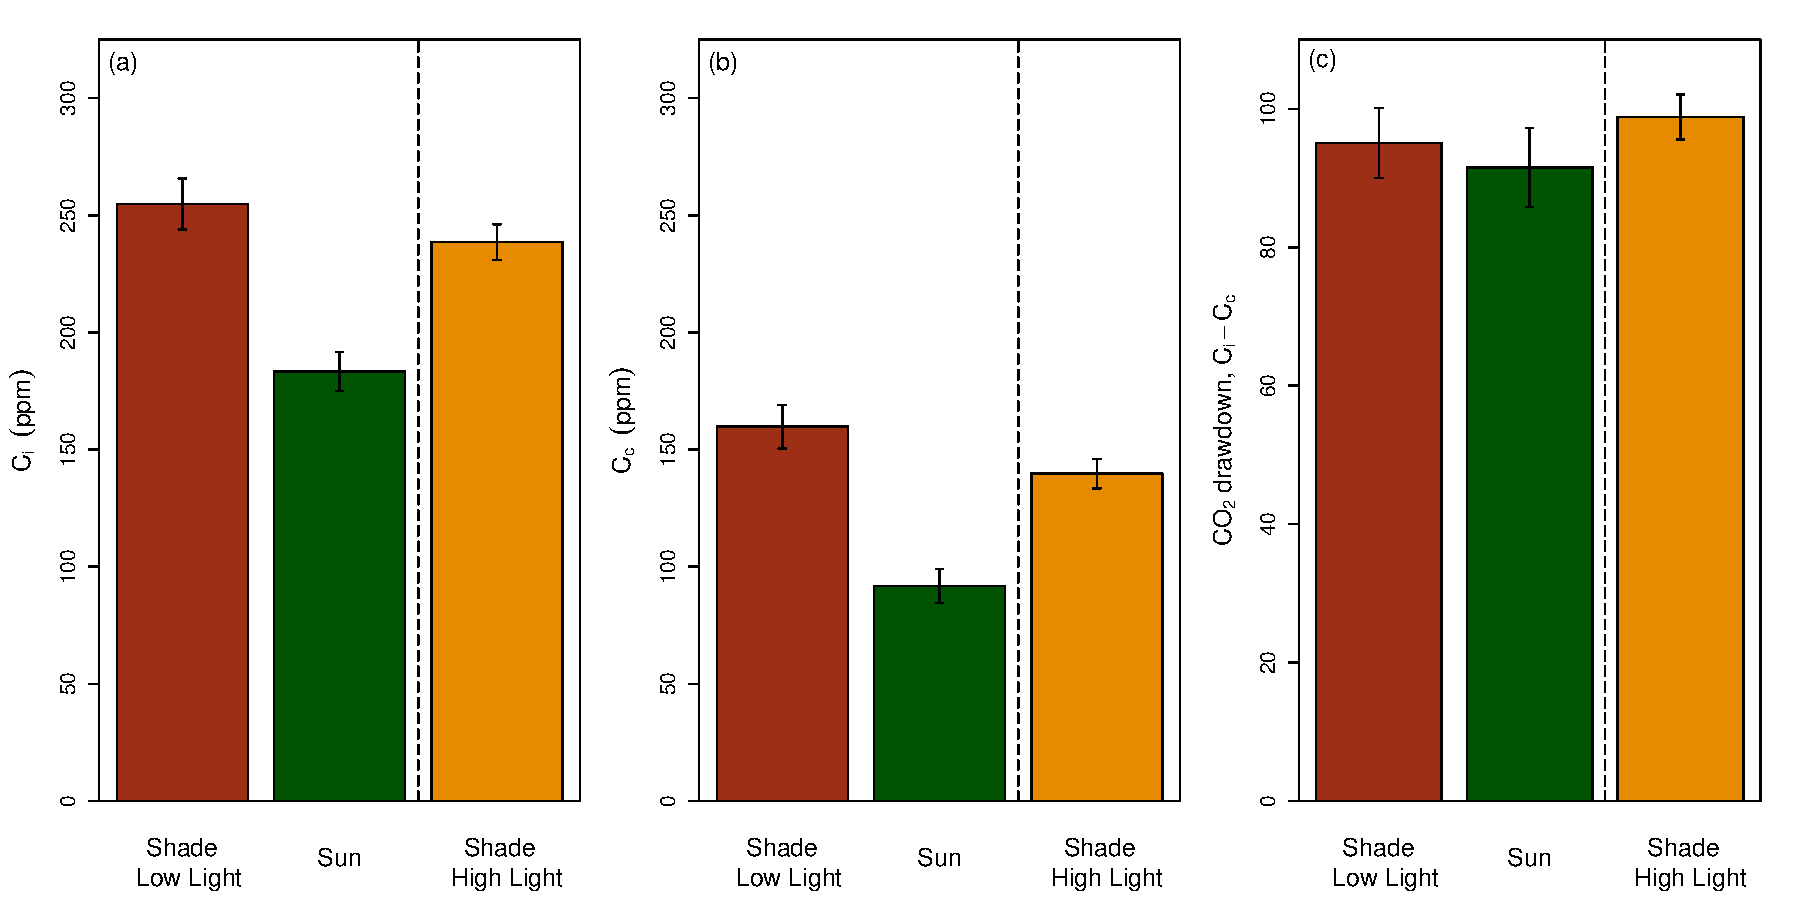
\includegraphics[width=0.99\textwidth]{cicc_bar.pdf}
    \caption{The mean $\pm$~1 standard error of intercellular CO\textsubscript{2} concentration (a), CO\textsubscript{2} concentration in the chloroplasts (b) and CO\textsubscript{2} drawdown from substomatal cavities to sites of carboxylation of sun leaves and shade leaves at both low and high light.}
    \label{fig:figure 3.7}
\end{figure}

\subsection*{DISCUSSION}
\subsection*{SUPPORTING INFORMATION}

%figure 3.S1
\begin{figure}[h!]
    \centering
    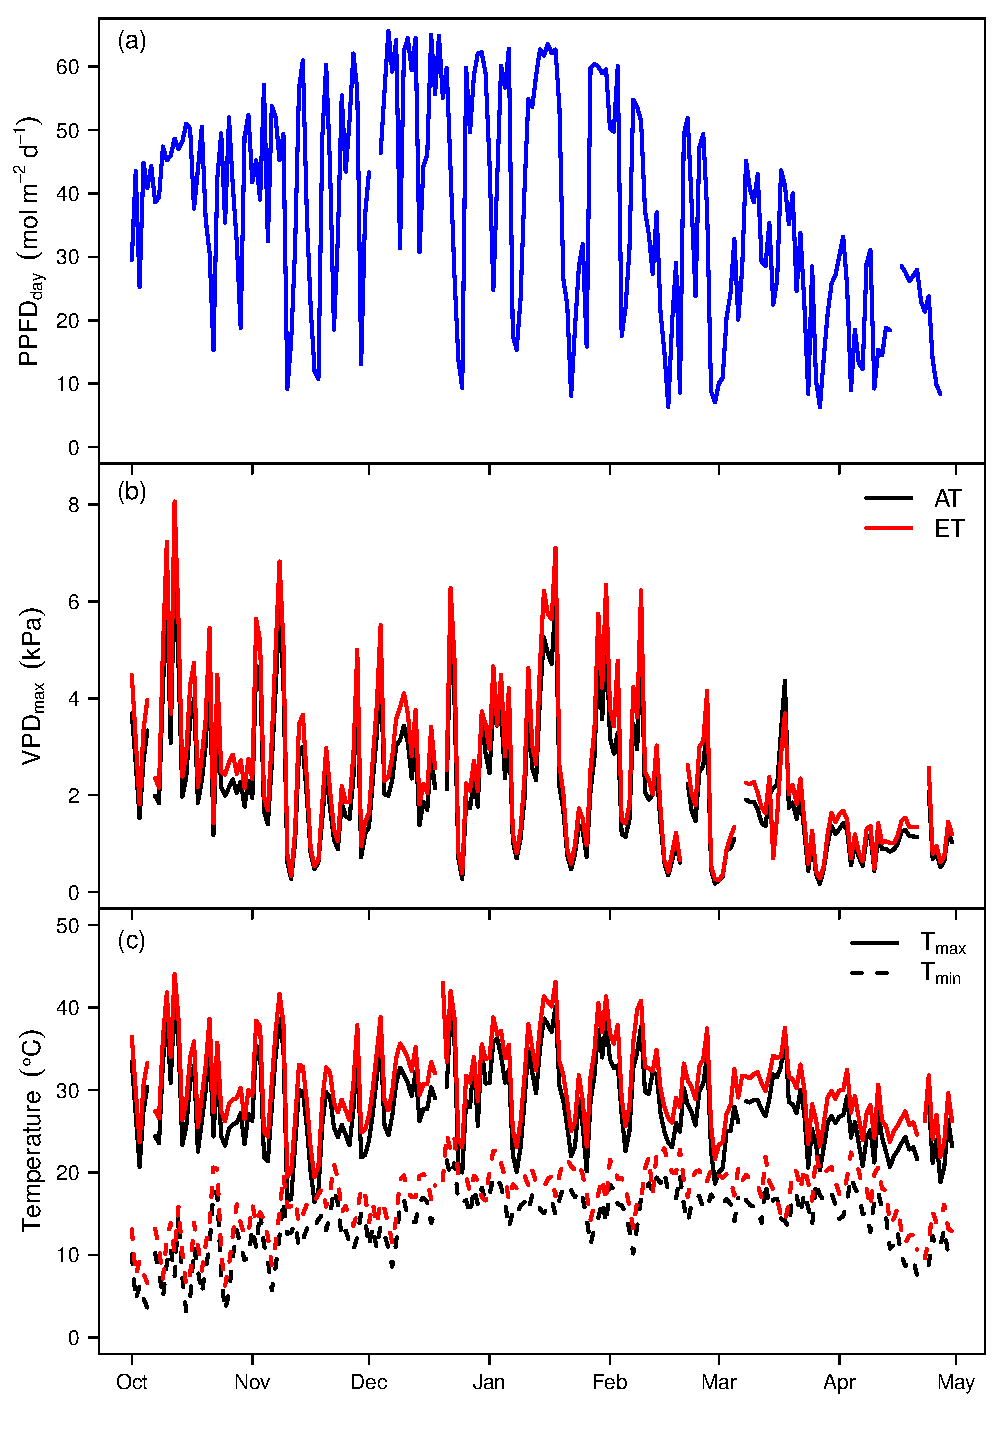
\includegraphics[width=0.99\textwidth]{airvars_wtc3.pdf}
    \caption{Daily maximum and minimum temperature (a) and total daily PPFD (b) for each chamber across the experiment duration.}
    \label{fig:figure 3.S1}
\end{figure}

%figure 3.S2
\begin{figure}[h!]
    \centering
    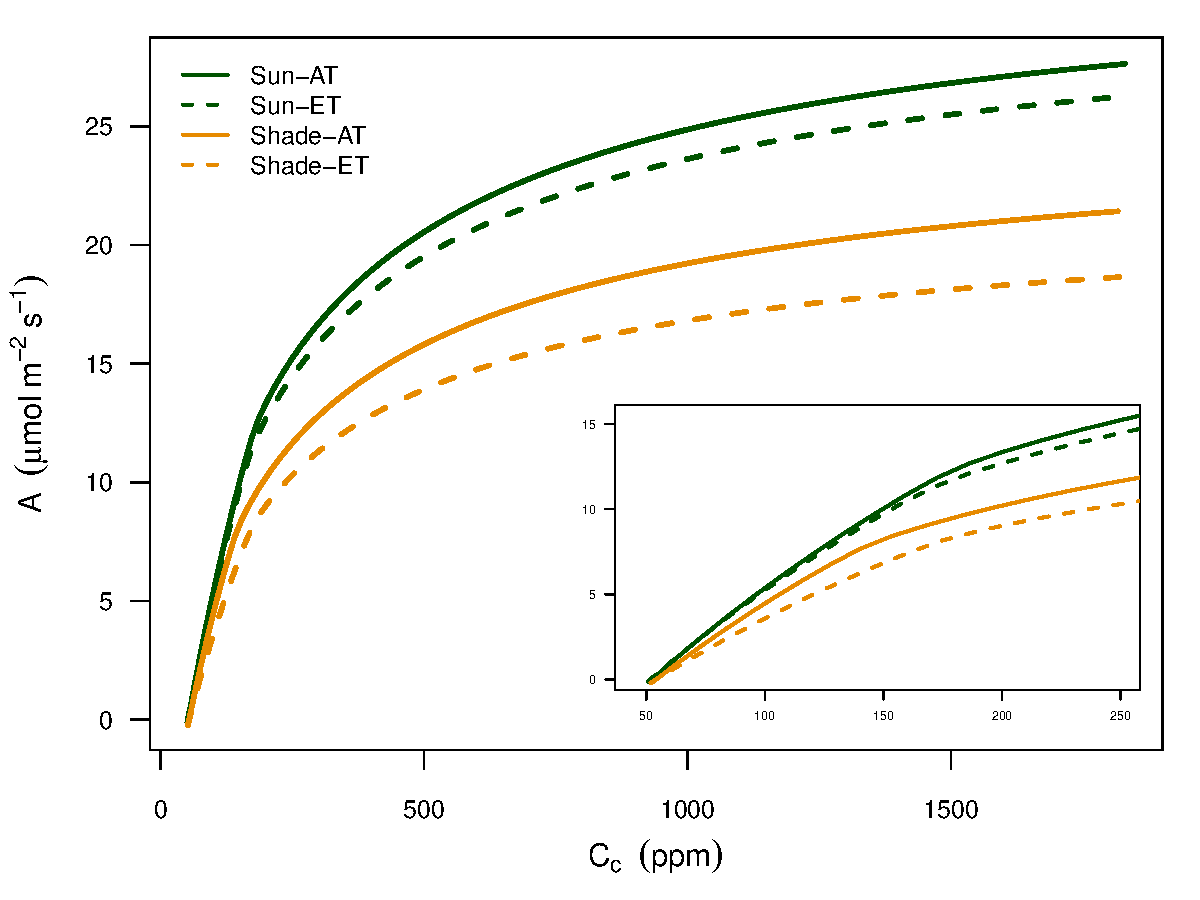
\includegraphics[width=0.99\textwidth]{Acc_model.pdf}
    \caption{Photosynthetic CO\textsubscript{2} response (AC\textsubscript{c}) curves for sun and shade leaves at elevated and ambient temperature treatments. C\textsubscript{c} values were predicted with g\textsubscript{m}, thus curves represent chloroplastic photosynthetic parameters at 25~$\degree$C and saturating light (1800~{\textmugreek}mol~m\textsuperscript{-1}~s\textsuperscript{-1}). }
    \label{fig:figure 3.S2}
\end{figure}

%figure 3.S3
\begin{figure}[h!]
    \centering
    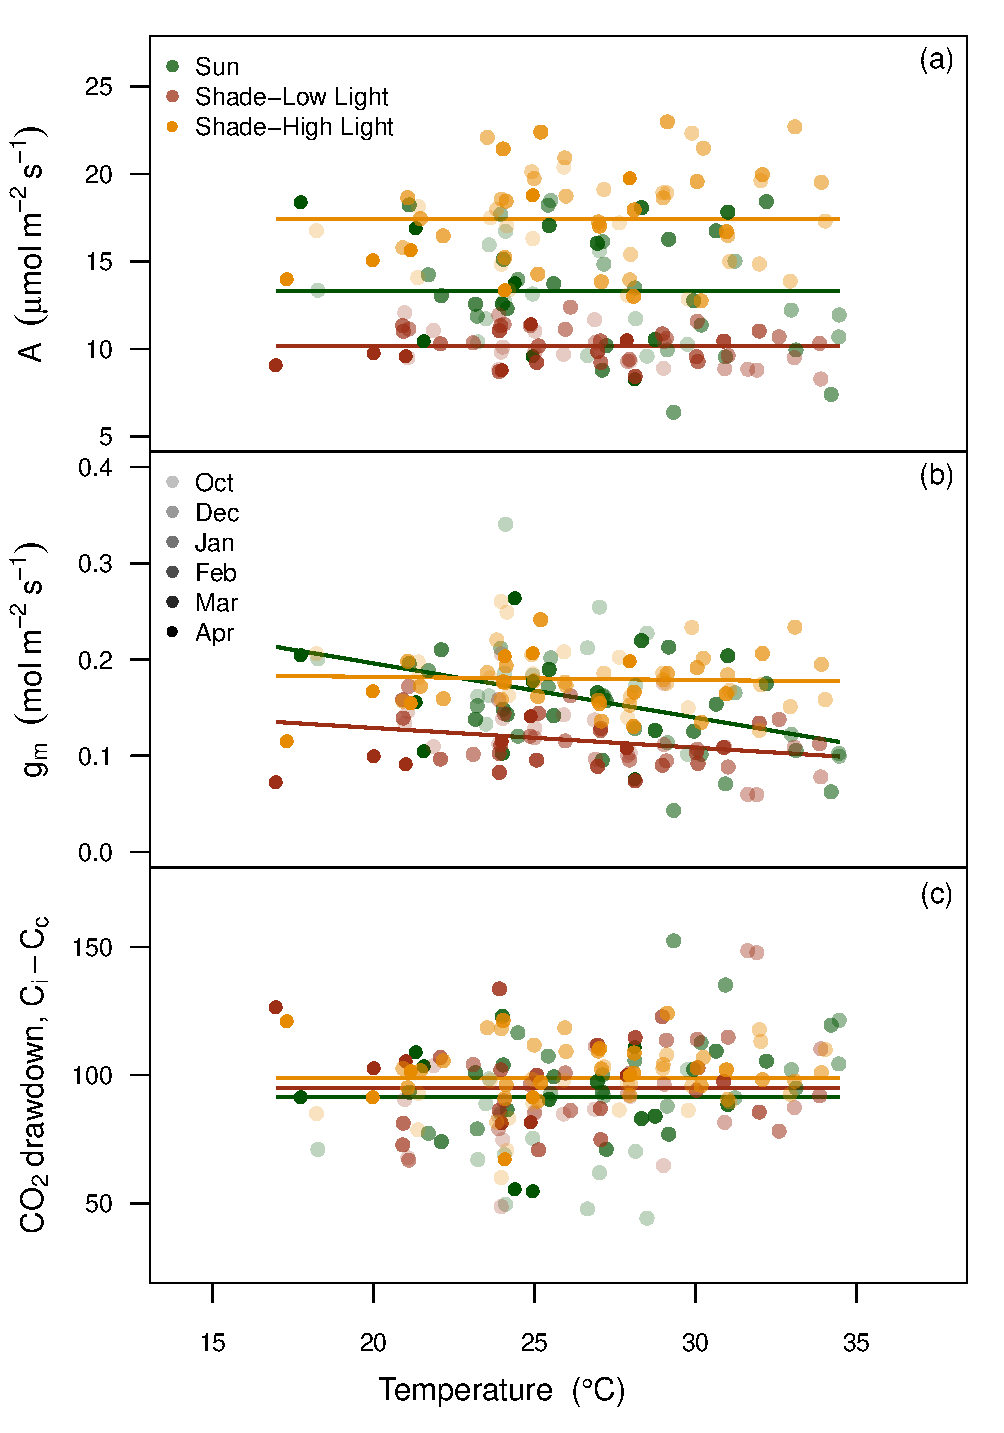
\includegraphics[width=0.99\textwidth]{gasex_temp3.pdf}
    \caption{Response of A (a), g\textsubscript{m} (b) and C\textsubscript{i}-C\textsubscript{c} to leaf temperature for sun leaves and shade leaves at low and high light. Shaded symbols represents each monthly measurement campaign. Solid lines, colored by leaf and light type, are fitted line for the relationship with each parameter and leaf temperature across all measurement campaigns. All parameters with no relationship are fitted with zero slope and the overall mean value for each treatment combination. Weak negative relationships with g\textsubscript{m} and increasing leaf temperature were detected with sun and shade leaves under their local light environment (R\textsuperscript{2}~=~0.16 and 0.08, respectively). }
    \label{fig:figure 3.S3}
\end{figure}

%figure 3.S4
\begin{figure}[h!]
    \centering
    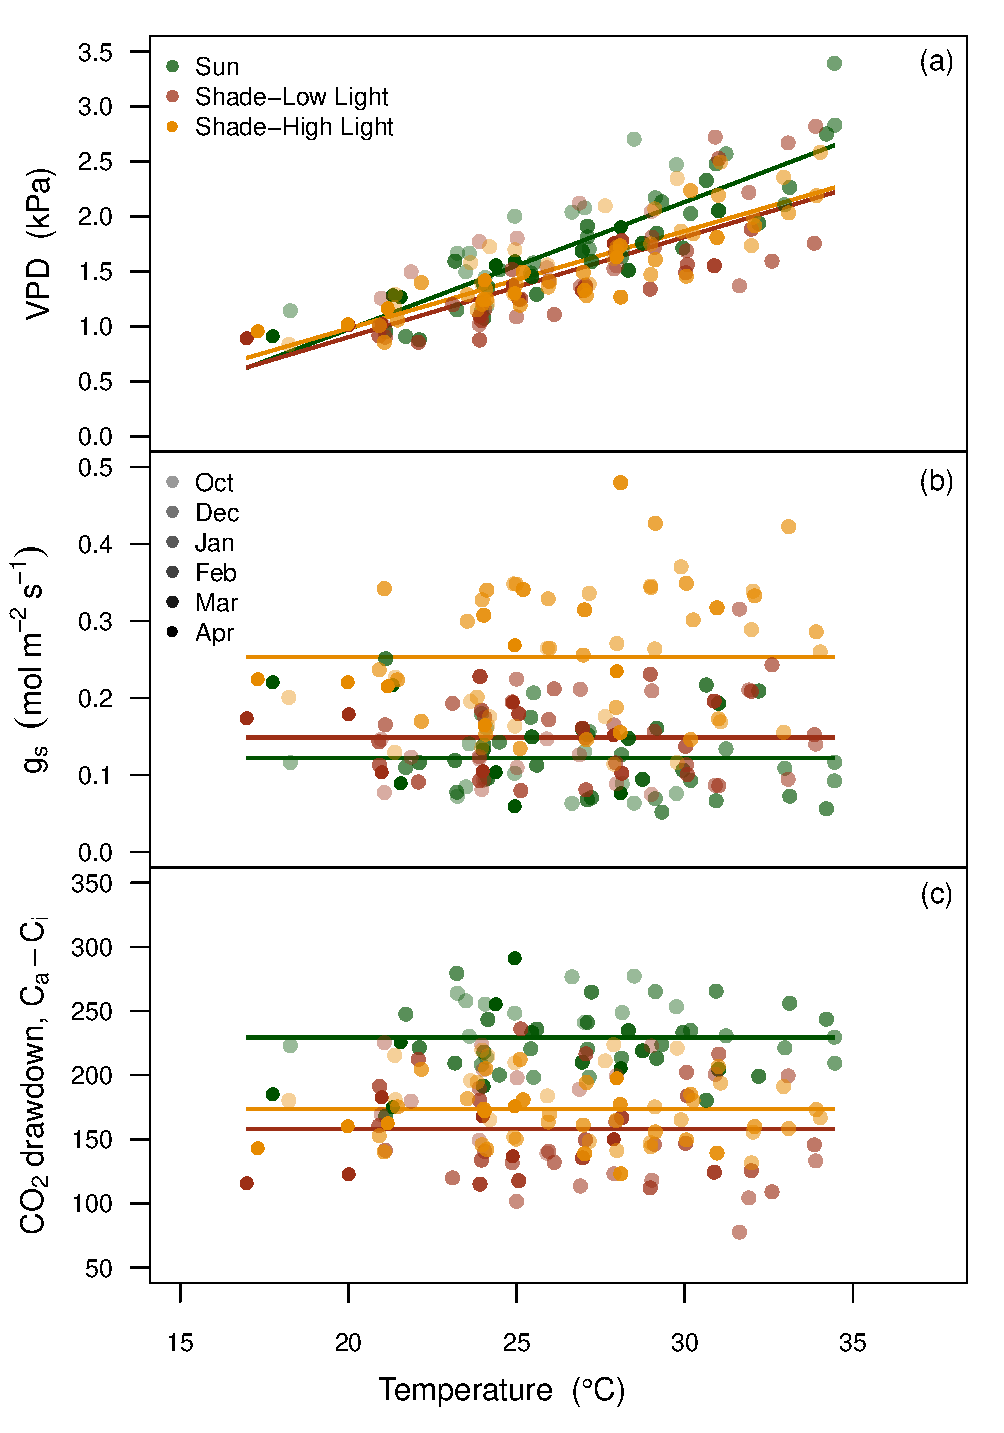
\includegraphics[width=0.99\textwidth]{gasex_temp4.pdf}
    \caption{Response of VPD (a), g\textsubscript{s} (b) and C\textsubscript{a}-C\textsubscript{i} to leaf temperature for sun leaves and shade leaves at low and high light. Shaded symbols represents each monthly measurement campaign. Solid lines, colored by leaf and light type, are fitted line for the relationship with each parameter and leaf temperature across all measurement campaigns. All parameters with no relationship are fitted with zero slope and the overall mean value for each treatment combination. Leaf VPD inside the gas exchange cuvette was positively correlated with increasing leaf temperature for sun leaves and shade leaves at low and high light (R\textsuperscript{2}~=~0.73, 0.58 and 0.72, respectively).}
    \label{fig:figure 3.S4}
\end{figure}



 

   
\addcontentsline{toc}{section}{CHAPTER 3 RAPID RESPONSE OF MESOPHYLL CONDUCTANCE TO LIGHT AVAILABILITY ALLOWS SHADE LEAVES TO TAKE ADVANTAGE OF SUNFLECKS}
\addcontentsline{toc}{subsection}{ABSTRACT}
\addcontentsline{toc}{subsection}{INTRODUCTION}
\addcontentsline{toc}{subsection}{MATERIALS AND METHODS}
\addcontentsline{toc}{subsection}{RESULTSS}
\addcontentsline{toc}{subsection}{DISCUSSION}
\addcontentsline{toc}{subsection}{SUPPORTING INFORMATION}
\clearpage
%--------------------------------------------------------------------------------------------%

% Load data for tables chapter 4



\section*{CHAPTER 4 \\ \mbox{ }\\ Elevated atmospheric CO\textsubscript{2} and drought alter carbon allocation above but not belowground in \textit{Eucalyptus saligna}}
\subsection*{ABSTRACT}
\subsection*{INTRODUCTION}
\subsection*{MATERIALS AND METHODS}


%figure 4.1
\begin{figure}[p!]
    \centering
    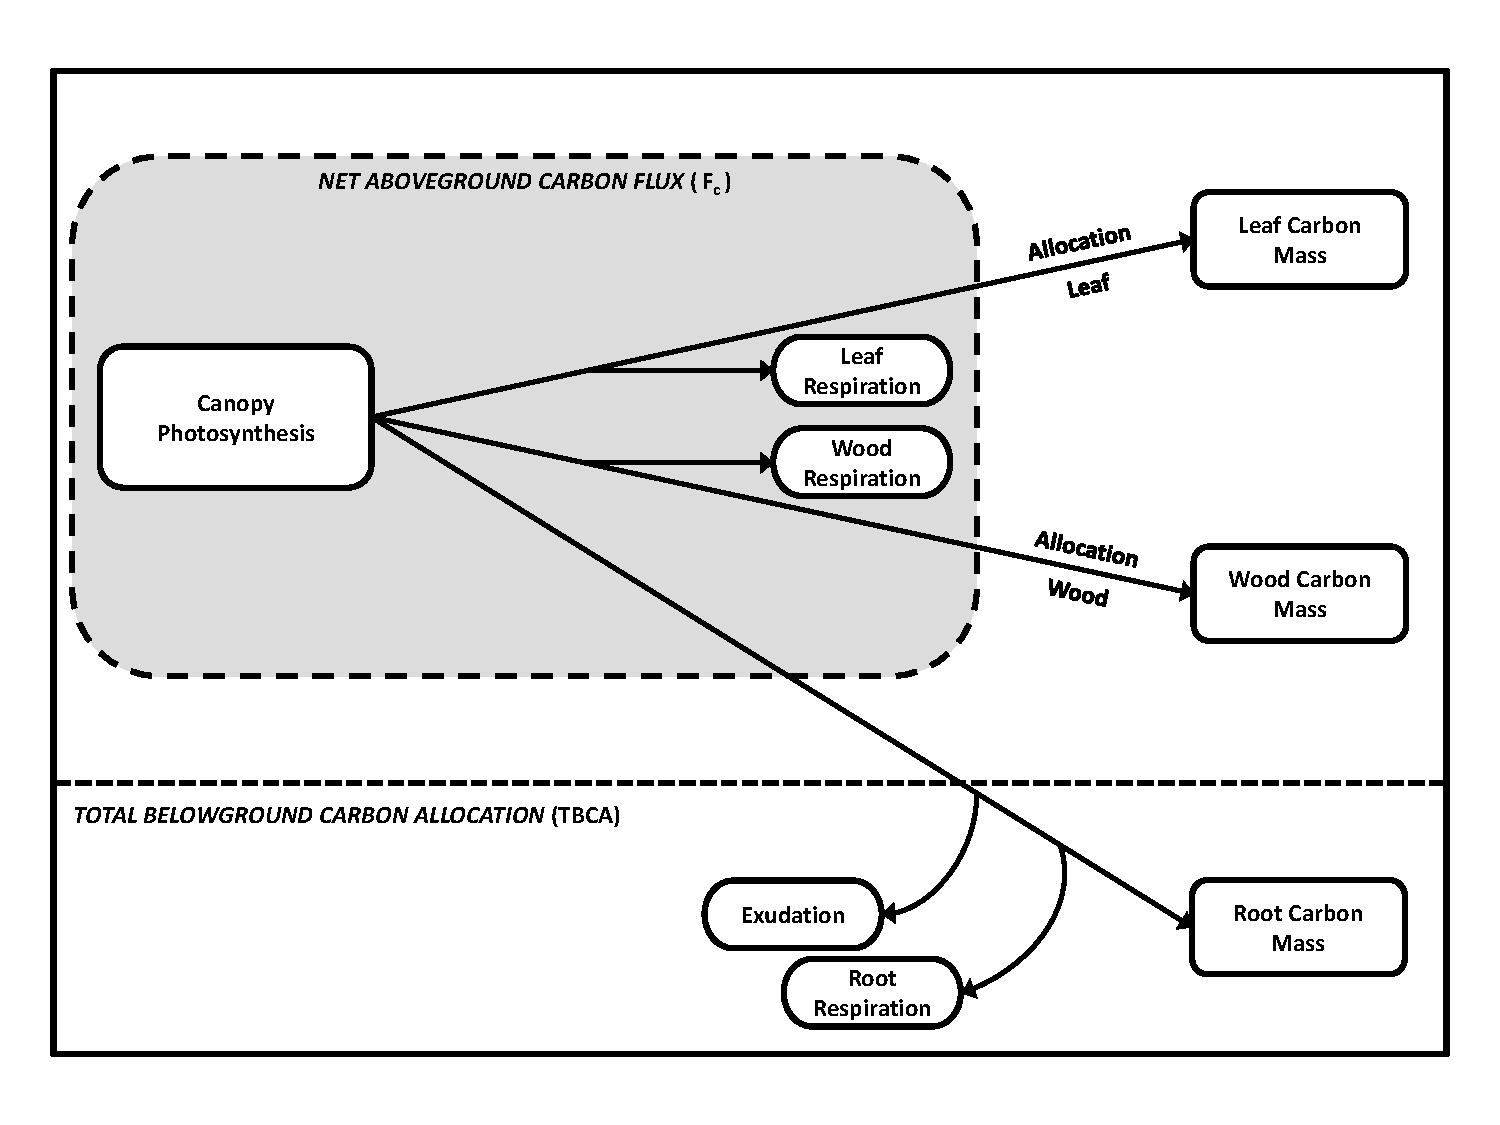
\includegraphics[width=0.99\textwidth]{conceptfig_wtc1.pdf}
    \caption{Conceptual diagram depicting the major components of C flow among plant components including; uptake via photosynthesis, allocation to component tissues, tissue respiration and root exudation. Net aboveground C uptake (F\textsubscript{c,T}), shown in the shaded box, represents the flux of C measured within each WTC. With the WTC experimental design, total belowground C allocation (TBCA) is measured as the residual between F\textsubscript{c,T} and total aboveground C mass. }
    \label{fig:figure 4.1}
\end{figure}

\subsection*{RESULTS}


%figure 4.2
\begin{figure}[h!]
    \centering
    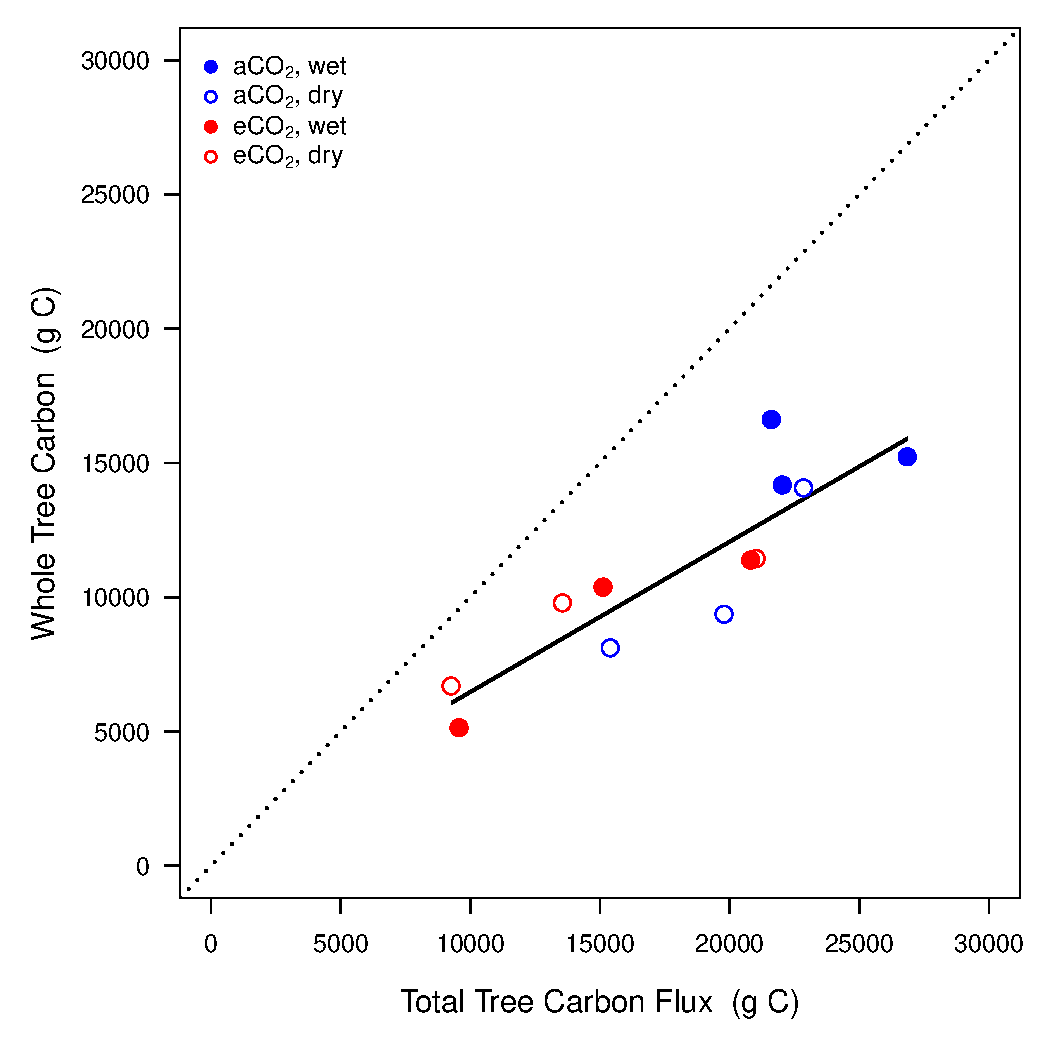
\includegraphics[width=0.99\textwidth]{flux_treecarbon3.pdf}
    \caption{Whole tree C mass as a function of cumulative aboveground C flux for each WTC tree. Values of cumulative aboveground net C flux were measured over the final eleven months of the experiment. Whole tree C mass represents the sum of bole, branch, leaf and root C mass from allometric estimates over the same time period. The dotted line is the 1:1 relationship and the solid line represents the significant overall linear model fit from the equation y = 0.56x + 878.2 (R\textsuperscript{2}~=~0.86).}
    \label{fig:figure 4.2}
\end{figure}

%figure 4.3
\begin{figure}[h!]
    \centering
    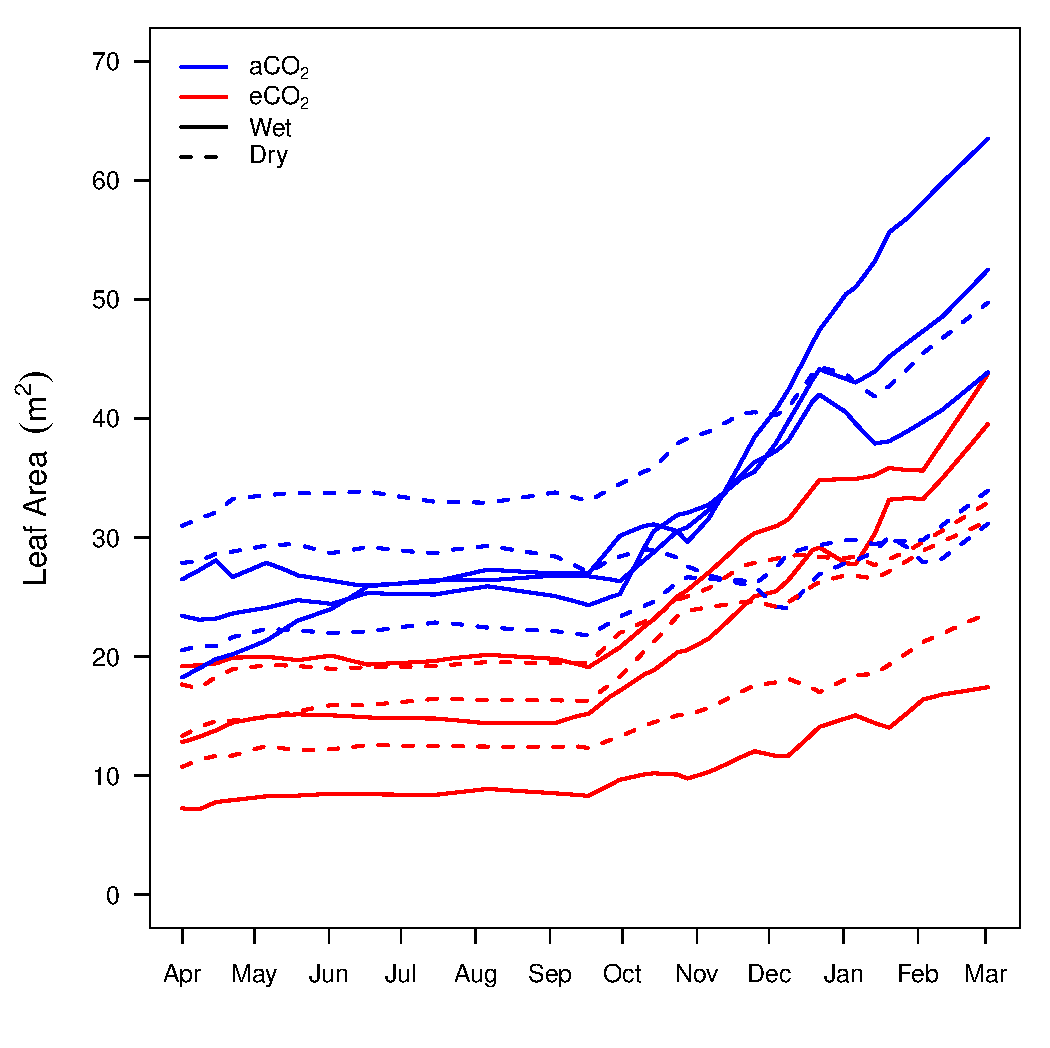
\includegraphics[width=0.99\textwidth]{leafarea.pdf}
    \caption{Estimated canopy leaf area for each WTC tree over the final eleven months of the experiment (April 2008 to March 2009). Estimates are based on height growth, litterfall rates and two leaf area estimates following \citet{barton2012effects}. Color and line type distinguish the treatment combination for each WTC.}
    \label{fig:figure 4.3}
\end{figure}

%figure 4.4
\begin{figure}[h!]
    \centering
    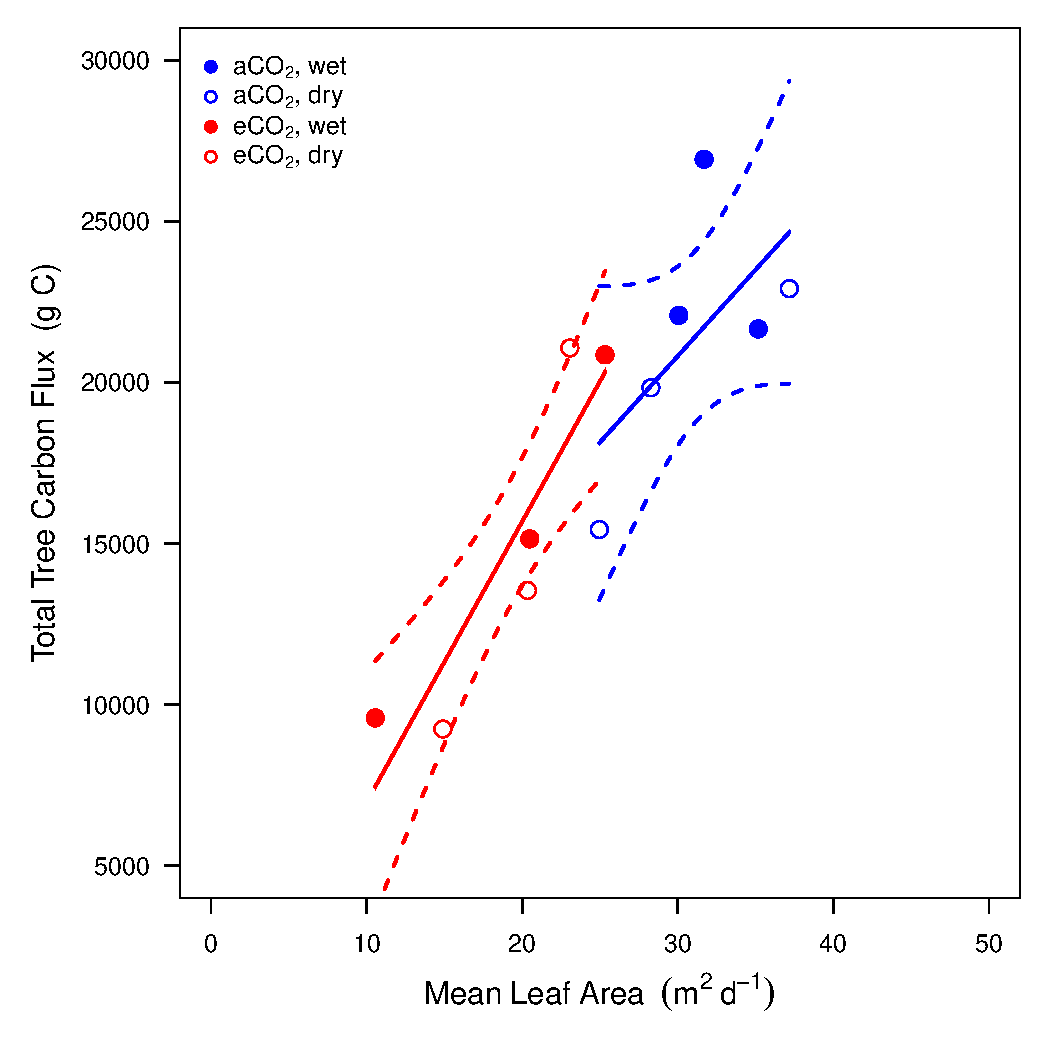
\includegraphics[width=0.99\textwidth]{flux_leafarea_co2.pdf}
    \caption{Treatment means of cumulative aboveground C flux as a function of mean daily canopy leaf area over the final eleven months of the experiment. The solid line represents the significant overall linear model fit (R\textsuperscript{2}~=~0.77) from the equation: y = 611.9x + 2791.2. Separate 95\% confidence intervals are shown for linear regression between F\textsubscript{c,T} and mean leaf area for aC\textsubscript{a} and eC\textsubscript{a} treatments.}
    \label{fig:figure 4.4}
\end{figure}

%figure 4.5
\begin{figure}[h!]
    \centering
    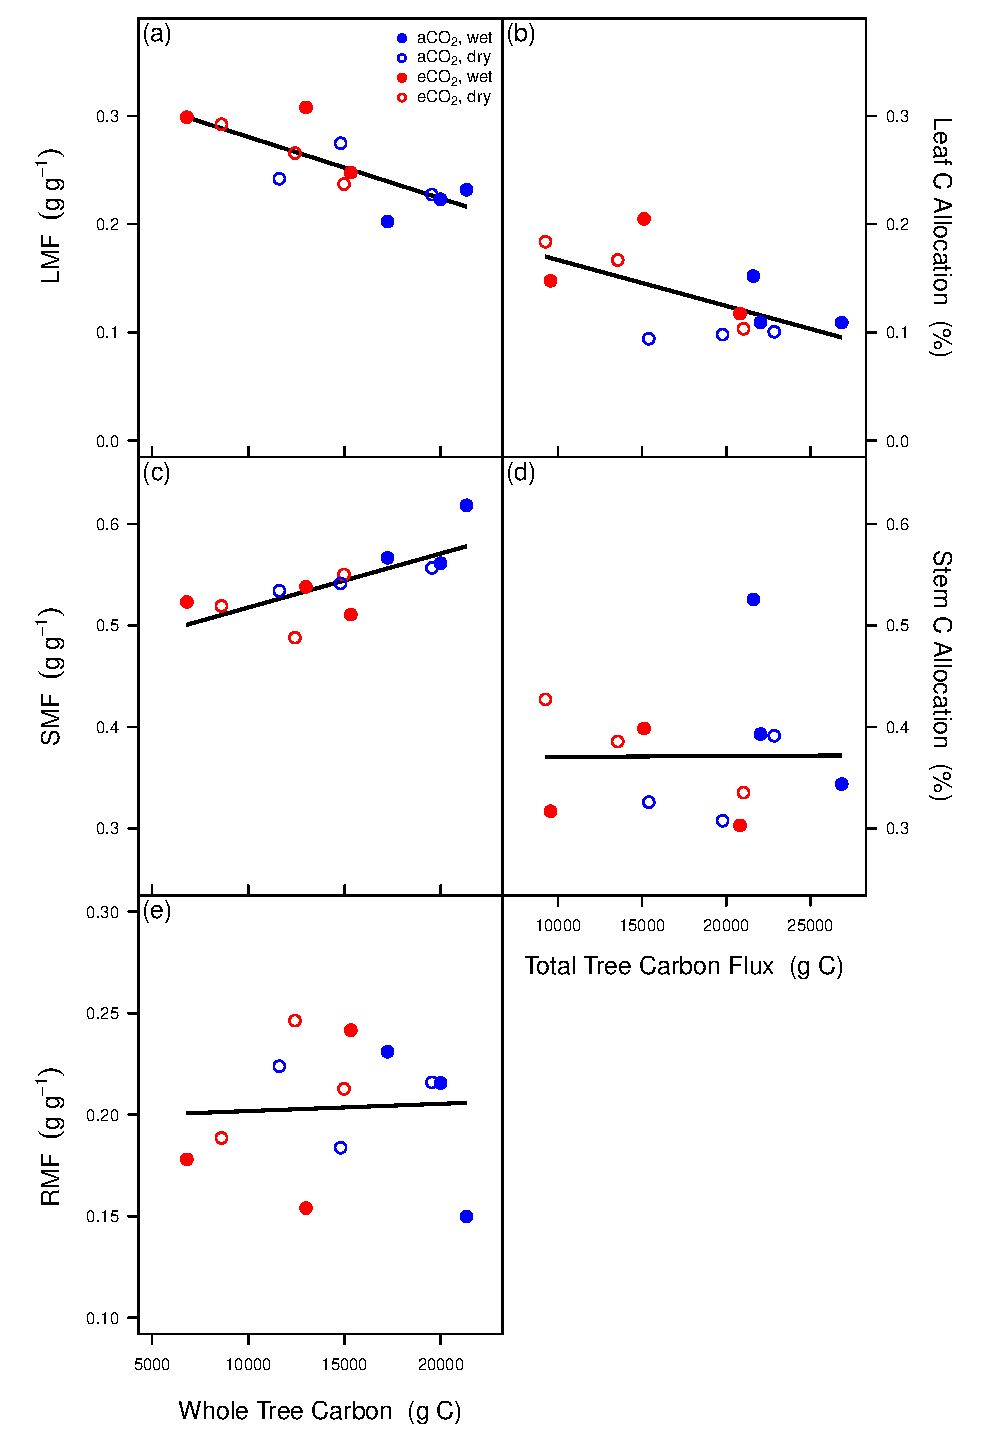
\includegraphics[width=0.99\textwidth]{allocfractions.pdf}
    \caption{Treatment means of C mass fractions of leaves (a), stems (branches+boles) (c) and roots (e) as a function of tree size, via whole tree C mass. Treatment means of C allocation to leaves (b) and stems (d) as a function of cumulative aboveground net C flux. Root C allocation could not be estimated as root turnover was not known. Values for C mass fractions are calculated from final harvest biomass totals. Values for C allocation are estimated from cumulative total aboveground net C flux over the final eleven months of the experiment. Solid lines represent overall linear model fit for leaf, stem and root mass fractions (R\textsuperscript{2} = 0.53,~0.26~and~0.01, respectively), as well as leaf and stem C allocation (R\textsuperscript{2}= 0.39, 0.01, respectively).}
    \label{fig:figure 4.5}
\end{figure}

%figure 4.6
\begin{figure}[h!]
    \centering
    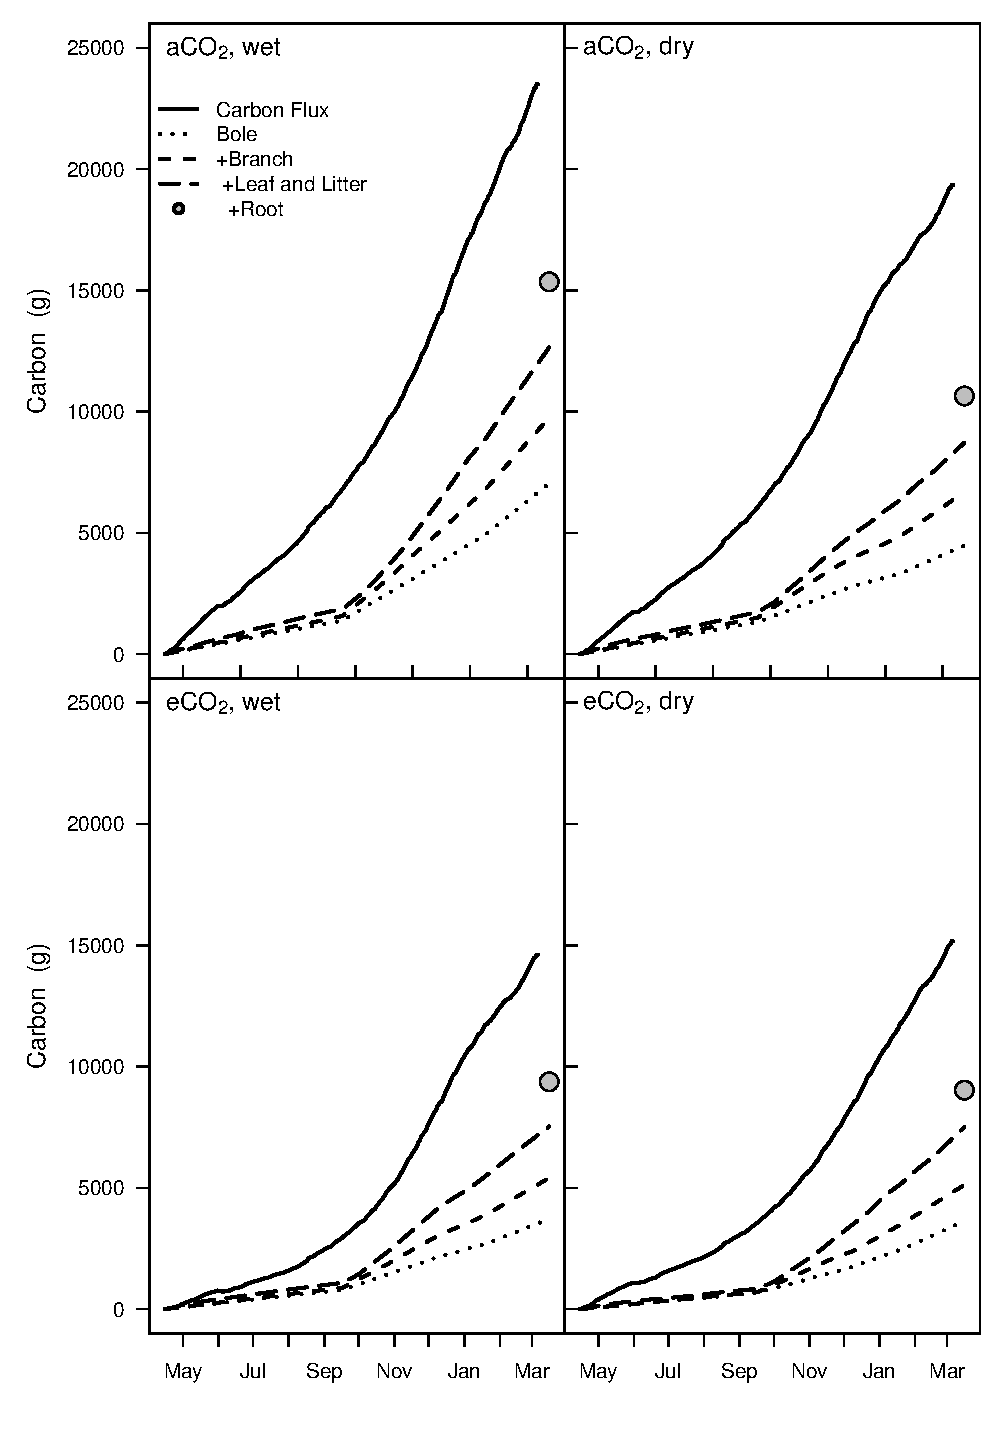
\includegraphics[width=0.99\textwidth]{treecarbon_daily2.pdf}
    \caption{Cumulative aboveground net C flux and additive C allocation to individual tree components from 15 April 2008 to 16 March 2009. Each panel represents mean values for each treatment combination (n=3). Both aboveground net C flux and tissue C allocation where set to 0 on 15 April 2008 in order to track the allocation of C in daily time steps. Root C mass, predicted from the logarithmic relationship between above and belowground mass partitioning of pre-planting seedlings and harvested trees, is shown on the last date.}
    \label{fig:figure 4.6}
\end{figure}

%figure 4.7
\begin{figure}[h!]
    \centering
    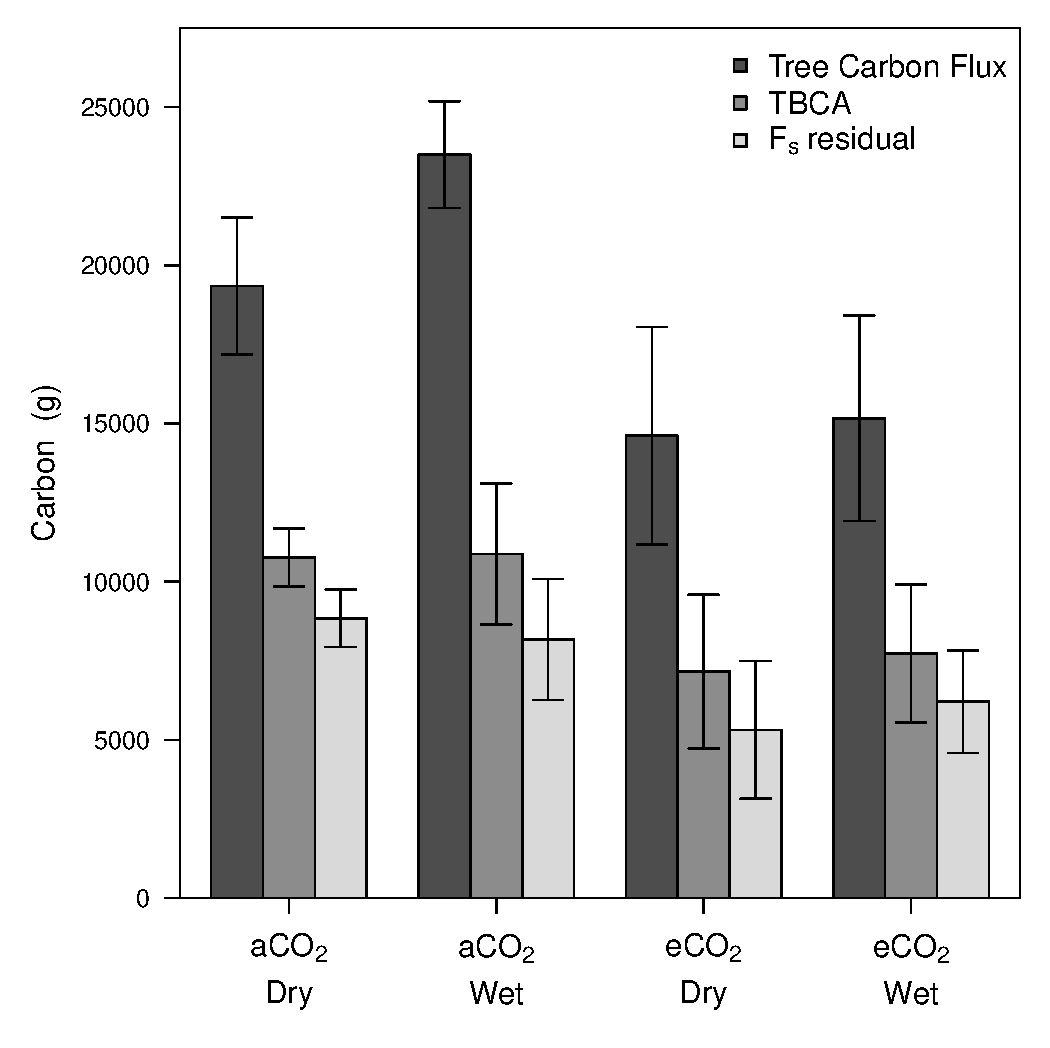
\includegraphics[width=0.99\textwidth]{belowground_flux_plots2.pdf}
    \caption{Treatment means $\pm$~1 standard error of cumulative aboveground net C flux, TBCA, and the residual belowground C flux (F\textsubscript{c,r}). Values of cumulative aboveground net C flux were measured over the final eleven months of the experiment. Values for TBCA are the residual between the cumulative C flux and total C mass aboveground estimated from allometric surveys over the same time period. Values for F\textsubscript{c,r} were calculated as the residual between TBCA and root C mass predicted on the last date of the eleven month period.}
    \label{fig:figure 4.7}
\end{figure}

%figure 4.8
\begin{figure}[h!]
    \centering
    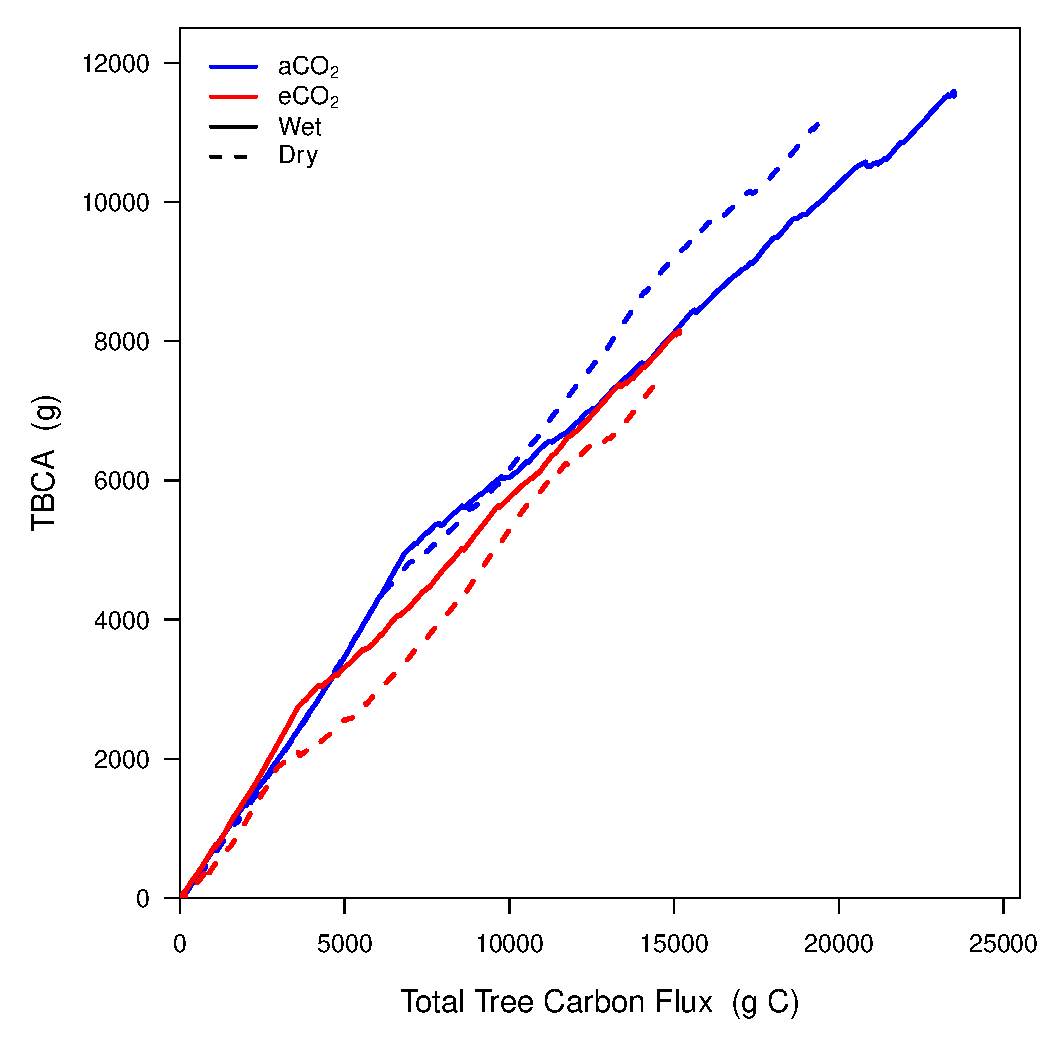
\includegraphics[width=0.99\textwidth]{tbca_cflux.pdf}
    \caption{Total belowground C allocation as a function of cumulative aboveground net C flux across the final eleven months of the experiment. Carbon mass aboveground was estimated from allometric surveys, interpolated on a daily time scale and then subtracted from the aboveground net C flux to quantify TBCA. Individual lines represent treatment means, with color and line type distinguishing treatment combinations.}
    \label{fig:figure 4.8}
\end{figure}


%wtc1tab
% latex table generated in R 3.2.3 by xtable 1.8-0 package
% Fri Dec 18 10:59:59 2015
\begin{sidewaystable}[ht]
\centering
\caption{Final harvest C mass of above and belowground tissues, cumulative aboveground tree C uptake (F\textsubscript{c,T}) and specific leaf area (SLA). Each value represents the mean ($\pm$~1 standard error) for each treatment combination. Units for C mass and F\textsubscript{c,T} are g~C, while SLA are cm\textsuperscript{2}~g\textsuperscript{-1}. For each variable, different letters represent significant differences between treatments from the overall model which includes CO\textsubscript{s} * drought interactions. P values represent overall differences of CO\textsubscript{s} or drought main effects and the CO\textsubscript{s} * drought interaction.} 
\label{table:Table 4.1}
\begin{tabular}{llllllll}
  \hline
Treatment & Bole & Branch & Leaf & Litter & Root & Tree.C.flux & SLA \\ 
  \hline
aCO\~{}2\~{}-dry & 5231.8 (687.0) b & 2799.2 (628.3) a & 2642.8 (370.7) a & 1129.8 (336.0) a & 3052.9 (500.2) a & 19394.2 (2169.5) a & 83.2 (3.3) a \\ 
  aCO\~{}2\~{}-wet & 7785.1 (267.1) ab & 3154.6 (687.1) a & 3254.2 (393.5) a & 1043.1 (47.3) a & 3677.4 (316.8) a & 23556.5 (1689.0) a & 87.9 (2.8) a \\ 
  eCO\~{}2\~{}-dry & 4080.5 (682.5) a & 1926.0 (369.4) a & 2232.1 (235.4) a & 889.4 (82.6) a & 2518.7 (481.6) a & 14620.7 (3456.2) a & 70.6 (3.6) a \\ 
  eCO\~{}2\~{}-wet & 4026.3 (783.3) a & 1856.8 (474.5) a & 2358.3 (473.6) a & 919.0 (244.3) a & 2213.9 (705.8) a & 15197.9 (3253.5) a & 81.8 (6.1) a \\ 
   \hline
CO\~{}2\~{} effect (P) & 0.005 & 0.086 & 0.122 & 0.417 & 0.091 & 0.044 & 0.053 \\ 
  Drought effect (P) & 0.085 & 0.803 & 0.358 & 0.897 & 0.766 & 0.413 & 0.089 \\ 
  CO\~{}2\~{} * Drought (P) & 0.075 & 0.712 & 0.539 & 0.792 & 0.397 & 0.532 & 0.454 \\ 
   \hline
\end{tabular}
\end{sidewaystable}



\subsection*{DISCUSSION}
\subsection*{SUPPORTING INFORMATION}

%figure 4.S1
\begin{figure}[h!]
    \centering
    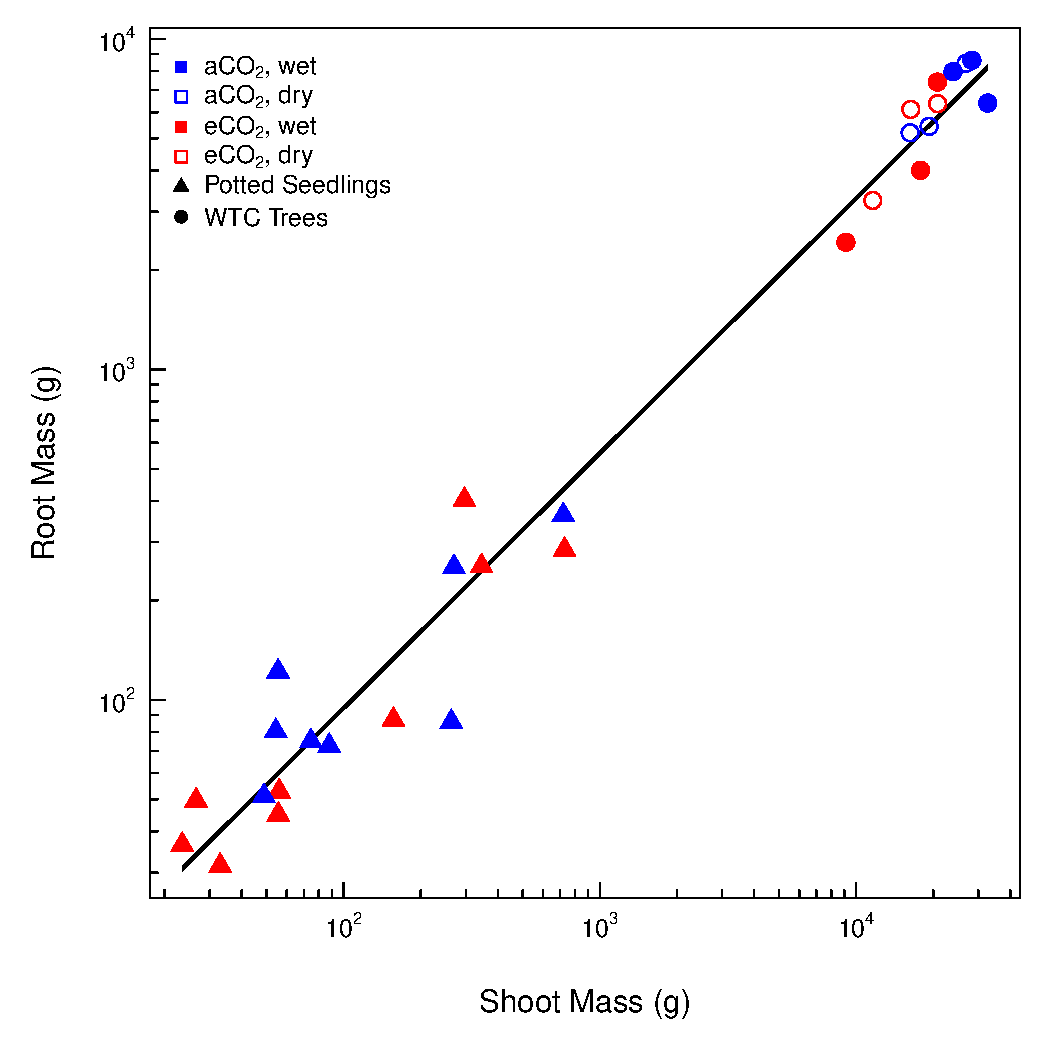
\includegraphics[width=0.99\textwidth]{rootshoot.pdf}
    \caption{Root mass as a function of shoot mass in \textit{Eucalyptus saligna} for potted seedlings harvested before planting of WTC trees (n=17) and WTC trees harvested after 2 years (n=12). Potted seedlings were grown in 25 l pots inside each WTC, while chamber [CO\textsubscript{2}] treatments conditions were maintained. The solid line represents the significant log-log model fit (R\textsuperscript{2} = 0.98) from the equation: log(x) = 0.77(log(y)) + 0.43.}
    \label{fig:figure 4.S1}
\end{figure}

%figure 4.S2
\begin{figure}[h!]
    \centering
    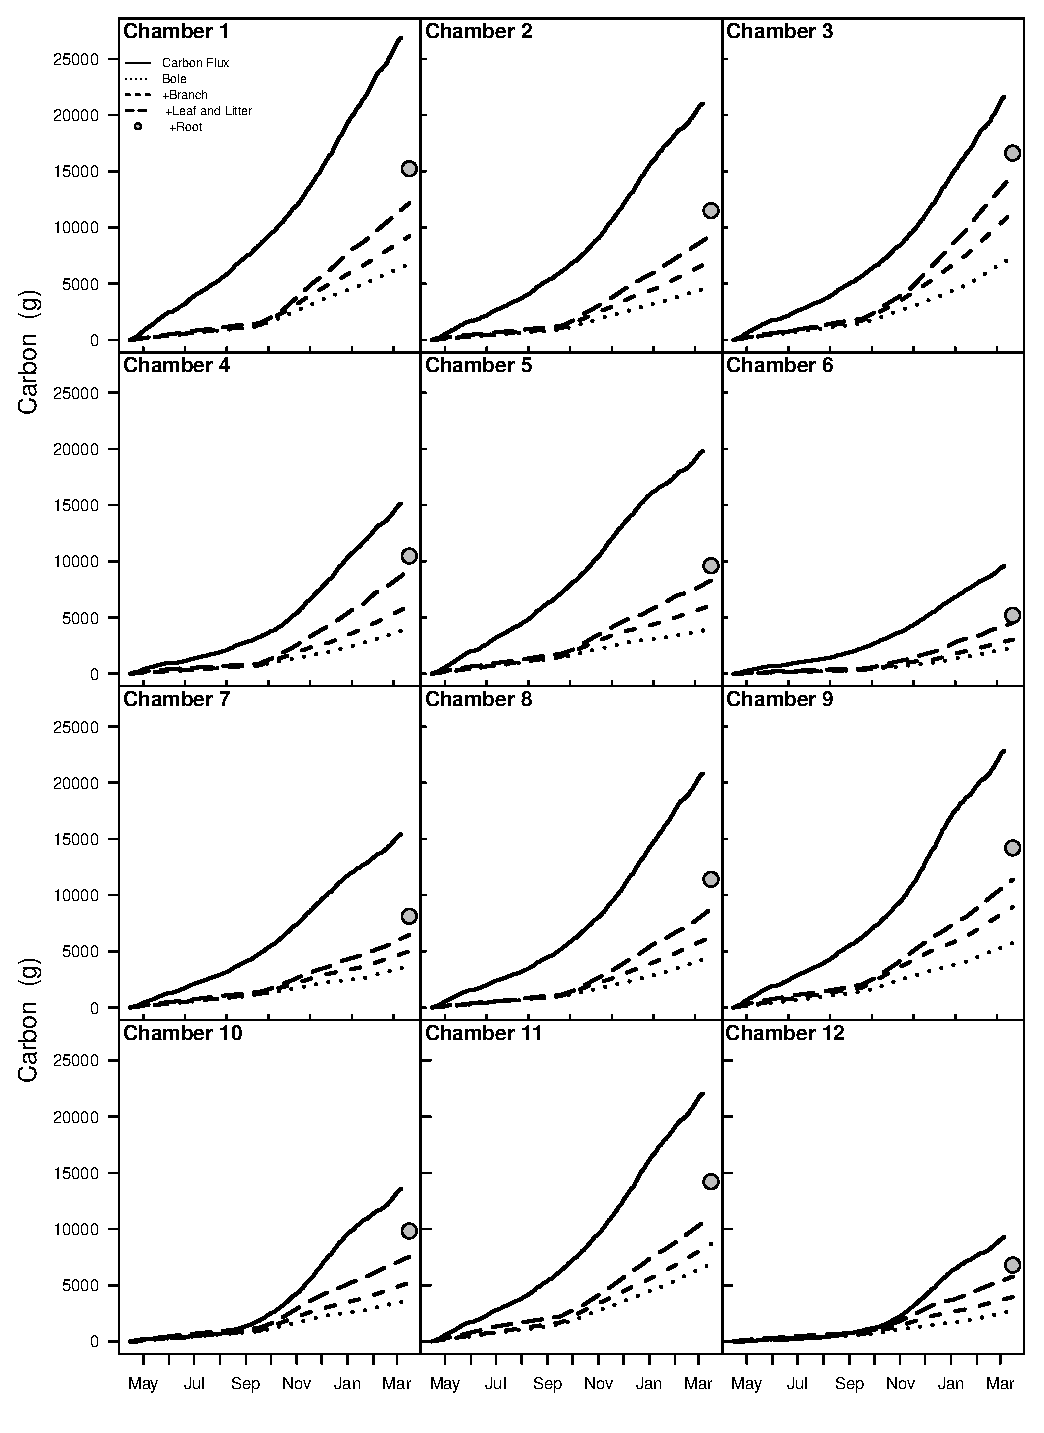
\includegraphics[width=0.99\textwidth]{treecarbon_daily_chambers2.pdf}
    \caption{Cumulative aboveground net C flux and additive C allocation of individual tree components from 2008-4-15 and 2009-3-16. Panels represent each individual WTC. Both aboveground net C flux and tissue C allocation where set to 0 on 2008-4-15 in order to track the allocation of C in daily time steps. Total root C mass, predicted from the log relationship between above and belowground mass partitioning of pre-planting seedlings and harvested trees, is shown on the last date.}
    \label{fig:figure 4.S2}
\end{figure}


\pagenumbering{arabic}
\setcounter{page}{1}     
\addcontentsline{toc}{section}{CHAPTER 1 ELEVATED ATMOSPHERIC CO\textsubscript{2} AND DROUGHT ALTER CARBON ALLOCATION ABOVE BUT NOT BELOWGROUND IN \textit{EUCALYPTUS SALIGNA}}
\addcontentsline{toc}{subsection}{ABSTRACT}
\addcontentsline{toc}{subsection}{INTRODUCTION}
\addcontentsline{toc}{subsection}{MATERIALS AND METHODS}
\addcontentsline{toc}{subsection}{RESULTSS}
\addcontentsline{toc}{subsection}{DISCUSSION}
\addcontentsline{toc}{subsection}{SUPPORTING INFORMATION}
\clearpage
%--------------------------------------------------------------------------------------------%
\section*{CHAPTER 5 \\ \mbox{ }\\ SYNTHESIS AND CONCLUSIONS}
\subsection*{SYNTHESIS}
It has long been recognized that resources limit plant growth in different environments, at different life stages and individual plant processes are limited by different resources \citep{bazzaz2000reproductive}. Consequently, a quantitative understanding of how plants gain and allocate resources is necessary to predict their success in any environment [@mooney1972carbon]. In this thesis, resources allocated for growth in \textit{Eucalyptus} tree species are classified into two distinct groups. The first group consists of environmental plant resources, such as N and H\textsubscript{2}O, that are captured, distributed and utilized to drive rates of leaf photosynthesis (\textit{A\textsubscript{n}}) and thus tree C gain. These C assimilates comprise the second group, which are the essential internal resource required for tissue growth, storage and to fuel respiration. These two resource groups are inextricably linked and interact to define plant growth across spatial and temporal scales. For example, the C expended in acquiring N makes up a significant fraction of the total energy a plant consumes, while leaf N investment constrains photosynthetic capacity \citep{chapin1987plant}. In trees, rates of \textit{A\textsubscript{n}} will then depend on the photosynthetic light response of individual leaves and the energetic trade-offs of gas exchange related to transpiration and water supply \citep{givnish1988adaptation}.

The research presented in this thesis was designed to investigate resource allocation in trees at individual tissue and whole plant scales in \textit{Eucalyptus}. I sought to address theories of plant functional balance by testing biomass partitioning in seedlings and trees undergoing various environmental manipulations. As observed biomass production may not necessarily reveal shifts in plant functional responses to environmental change, I evaluated the sensitivity of the allocation of photosynthate above and belowground across different temporal scales. Using mass balance approaches I then tested the coordination between growth and \textit{A\textsubscript{n}}, using leaf gas exchange parameters in seedlings and measurements of net canopy C gain in trees. To help bridge the knowledge gap between leaf and canopy C gain I investigated the distribution of N and H~\textsubscript{2}O as a function of light availability within canopies and the effect this has on individual leaf physiology. By utilizing novel experimental approaches, evidence from this work improves our understanding of functional processes that determine the net C uptake of trees and then how this assimilated C is used to fuel growth. The contribution of this body of work provides fundamental evidence underlying resource allocation in ecologically and commercially important \textit{Eucalyptus} tree species.

\subsubsection*{Where does the carbon go?}
This thesis question arises from large uncertainties that remain regarding fundamental processes which affect terrestrial C cycling.  The question \enquote{Where does the carbon go?} arises from the need to track the fate of C from canopy \textit{A\textsubscript{n}} to determine the contribution of forests ecosystems to C cycling \citep{litton2007carbon}. Currently, empirical data on C allocation are critical to the further development of forest models and subsequent predictions of global C balance under climate change \citep{franklin2012modeling}. Growth responses during early phases of tree establishment (seedlings or young trees) to changes in soil resource availability or climate change factors will likely depend on shifts in the plant C budget to balance growth, respiration and storage. Consequently, understanding environmentally driven shifts in C allocation in young *Eucalyptus* trees will be crucial to manage their fitness in fragile native ecosystems and their productivity in terms of timber production and quality in forestry systems.

First, I examined patterns in biomass partitioning of \textit{E.tereticornis} seedlings with belowground resource limitation (Chapter 1) and with \textit{E.saligna} trees exposed to eC\textsubscript{a} and drought treatments (Chapter 2). Across these studies, partitioning of biomass largely followed allometric trajectories related to plant size, nearly independent of treatment manipulation. Partitioning to roots, leaves and stems in \textit{E.tereticornis} seedlings was conserved across a ten-fold variation in seedling biomass with and without soil volume restriction. During this early growth stage, these results infer that growth inhibition from reduced belowground sink strength did not elicit a functional partitioning response. With much larger 2 year old \textit{E.saligna} trees, grown in WTCs, differences in partitioning to stem biomass were detected between aC\textsubscript{a} and eC\textsubscript{a} treatments. These patterns were also attributed to size dependent relationships associated with ontogeny \citep[see]{poorter2015does}, rather than a direct functional response to eC\textsubscript{a}.

Combined results from these two experiments argue against traditional views of plant functional balance in the context of observed biomass production. These theories posit that plants will \textquote{optimally forage} for the most limiting resource, thus shifts in biomass partitioning should occur. However, adaptive plant responses may not include changes in biomass production at any given \textquote{snapshot} in time.  This makes tracking C allocation to processes other than observed biomass just as important in assessing overall responses to manipulations of resource availability. Here, empirical and modelling evidence from Chapters 2 \& 4 reveal that detection in shifts of tissue C allocation were necessary to interpret whole tree response to environmental manipulations. For \textit{E.tereticornis} seedlings, modelling results infer that increases in C allocation to pools other than biomass were required to fully explain the effects of soil volume restriction on seedling growth. For \textit{E.saligna} trees, increased leaf C demand under eC\textsubscript{a} treatments resulted in higher C allocation to leaves without altering observed leaf biomass production. Overall, the ability to distinguish biomass production from C allocation across tissues reveals that alternate explanations are likely need to interpret the degree in which trees strive to maintain functional balance.

Alternatively, shifts in tissue morphology, metabolism or turnover to alter resource uptake of loss [@reich2002root], increased root exudation to alleviate resource limitation [@phillips2011enhanced] or increased C allocation to storage \citep{sala2012carbon, dietze2014nonstructural} may be used to balance trade-offs between tissue sink strength, resource availability and source C supply. Partial evidence for these \textquotesingle non-biomass\textquotesingle responses were evident in \textit{E.tereticornis} seedlings in research presented in Chapter 2. Increases in specific root length were detected in some, but not all, of seedlings with soil volume restriction. Modelling results also revealed that increases in tissue respiration rates were a possible mechanism to account for the oversupply of C not allocated to biomass. Increases in leaf carbohydrate storage were correlated with reduced belowground sink strength in these seedlings, and it is possible that C storage increased in other tissues. Although not measured, root exudation may have increased in response to adverse poor quality soil conditions with \textit{E.tereticornis} seedlings in containers or in \textit{E.saligna} trees under eC\textsubscript{a} to meet resource demand, but was not explicitly measured.

The ability to compare biomass partitioning with aspects of C allocation across multiple experiments highlights how partial accounting of C may lead to erroneous conclusions regarding adaptive plant responses to changing environments. Overall, these results reveal why studies using only biomass partitioning to assess functional balance or allometric based theories have mixed results. Additionally, shifts in above but not belowground C allocation \textit{E.saligna} trees disagrees with the common observation of enhancement of belowground processes in other trees species under eC\textsubscript{a} \citep[see]{palmroth2006aboveground, iversen2014terrestrial}. \citet{shipley2002balanced} states that it is more appropriate to state that plants shift biomass allocation to reduce imbalances between leaf source activity and tissue resource acquisition. Collectively, results from this research tend to agree with this conclusion, with the caveat that the concept of allocation must be extended to include fates of C other than measured biomass. Consequently, we agree with \citet{poorter2012biomass} that understanding C allocation above and belowground requires a better understanding of the interactions between tissue source and sink activity at any time point. In order to fully understand the impact environmental change has on forest productivity approaches to quantify patterns in C allocation must be prioritized in future studies.

\subsubsection*{When do photosynthesis and growth not add up?}

This thesis question addresses the debate over how strongly plant growth is controlled by either source or sink activity, which may disrupt the coordination between \textit{A\textsubscript{n}} and growth at different temporal scales. Assimilated C is first allocated to provide sufficient sucrose for the immediate demands of the plant during the day, and sufficient starch to meet \textquotesingle anticipated\textquotesingle demands during the following night \citep{smith2007coordination}. The C demands for each tissue, referred to as tissue C sinks, determine the C budget for the entire plant and regulate C allocation. Despite competition among highly integrated C sinks, woody plants also maintain storage carbohydrate pools as C reserves \citep{kozlowski1992carbohydrate}. Understanding the coordination between plant growth and \textit{A\textsubscript{n}} thus requires mass balance approaches to quantify the fractions of C supply allocated to growth, storage and respiration of different organs. Reductions in tissue sink strength have been shown to signal the down regulation of \textit{A\textsubscript{n}}, which can led to increased starch synthesis for storage \citep{sage1994acclimation, kitao2007interaction}. This had led to support for the argument that increased shifts to C storage will compete with C available for plant growth \citep{chapin1990ecology}, which may then disrupt the coordination between \textit{A\textsubscript{n}} and growth at short time scales.

To address this thesis question the belowground sink strength of \textit{E.tereticornis} seedlings was manipulated, through container size treatments, to test the effects of putative sink limitation on \textit{A\textsubscript{n}} and leaf TNC production (Chapter 1). Empirical results and modelling approaches were combined to test the coordination of A and growth of seedlings with and without soil volume limitation over 120 days. First, apparent reductions in belowground sink strength negatively impacted leaf N content and photosynthetic capacity, while leaf starch increased. These results support other findings where manipulation of tissue C sinks leads to carbohydrate accumulation and photosynthetic down regulation \citep{hoch2002altitudinal, iglesias2002regulation, equiza2006photosynthetic, urban2007girdling;, haouari2013fruit}. Second, large reductions of harvested biomass in seedlings with soil volume limitation initially suggested that observed reductions in \textit{A\textsubscript{n}} and growth were tightly linked. As previously shown in thesis Question 1, however, partial accounting of C allocation could lead to premature conclusions regarding this linkage. Importantly, using measured reductions in \textit{A\textsubscript{n}} with a mass balance seedling growth model largely over-predicted biomass production from observed results. These findings reveal that not only can \textit{A\textsubscript{n}} and growth not add up when belowground sink strength changes but other mechanisms, beyond \textit{A\textsubscript{n}} and carbohydrate accumulation, must now be explored to explain growth responses.

At long enough time scales, however, \textit{A\textsubscript{n}}and respiratory losses together determine net C balance and must be coordinated to plant growth. Consequently, we need to evaluate if trade-offs between storage and growth actually matter for long term C balance of trees \citep{palacio2014does}. The difficulty in measuring total canopy C uptake and the allocation of this assimilate to different tissue sinks currently impedes the ability to quantify whole tree C balance through time. Combining allometric approaches to estimate growth with seasonal variation in carbohydrates of stem wood and roots, \citet{genet2010age} found contrasting results with the C balance between storage and growth across a chronosequence of stand age. Utilizing the novel WTC experimental design, I sought to address this knowledge gap by applying a simple mass balance approach with \textit{E.saligna} trees (Chapter 4). Empirical measurements of net cumulative C uptake were correlated with whole tree C mass, which integrates the total allocation of C to growth and storage over an 11 month period. This simplified method allows for the coordination of \textit{A\textsubscript{n}} and growth to be tested with minimal issues in accounting for C retention in tissues through time. During this time period, total tree C mass was strongly correlated to net canopy photosynthetic C gain across a 2.5 fold range in tree size. Even though the the C balance between growth and storage was likely disrupted by eC\textsubscript{a} in these trees, it did not affect the overall coordination between C supply and growth over ~1 yr. Overall, results from Chapters 2 \& 4 highlight how utilization of C mass balance improves our ability to explore mechanisms in which source and sink activity feedback to tree growth. Although I show that answers to the debate regarding the coordination of allocation of C to storage and growth requires a deeper understanding C allocation, it appears that whole canopy assimilation and tree growth are tightly coordinated over long periods.

\subsubsection*{Are whole canopies optimized for carbon gain?}

Scaling from single leaf photosynthetic performance to net canopy assimilation is difficult because of concomitant variations in environment and foliage physiology and structure \citep{niinemets2009packing}. The ability to estimate whole canopy C gain involves knowledge of the non-linear responses of \textit{A\textsubscript{n}} to light between shaded and sunlit leaves \citep{de1997simple, linderson2012up}, which requires the ability to differentiate  light energy utilization, environmental resource distribution, physiological behavior and CO\textsubscript{2} fluxes within tree canopies \citep{dai2004two, peltoniemi2012co, niinemets2012optimization}. Theory suggests that interactions between traits which influence \textit{A\textsubscript{n}} and transpiration should interact to determine optimal patterns of behavior for whole plant C gain \citep{cgivnish1988adaptation}. Theories of optimal resource allocation and leaf physiological behavior have been developed \citep{cowan1977stomatal, medlyn2011reconciling, peltoniemi2012co} and subsequently tested \citep{wright2003least, heroult2013optimal, prentice2014balancing, lin2015optimal} across different ecosystems and plant functional types. This thesis question arises because optimal leaf physiology is commonly assessed for seedlings or \textquotesingle full sun\textquotesingle leaves, thus our understanding of how resource allocation and individual leaf physiology interact to maximize net canopy C uptake is surprisingly limited. Seeking answers to ecological questions such as \enquote{Where does the carbon go?} and \enquote{When do photosynthesis and growth not add up?} first requires an understanding of \enquote{Where is the carbon fixed?}.

Theories of leaf economic strategies are often used to describe the patterns in which resources are distributed in order for plants to optimize \textit{A\textsubscript{n}} \citep{wright2003least}. In this economic framework, I first evaluated how N and water supply were distributed in relation to photosynthetic capacity within \textit{E. tereticornis} tree canopies (Chapter 3). Leaf N and photosynthetic capacity were found to be highest in full sun leaves, which agree with conventional theory that resources for \textit{A\textsubscript{n}} should be preferentially invested relative to light availability. Overall, higher measured rates of \textit{A\textsubscript{n}} in full sun leaves compared to shade leaves implies that N resources were invested to maximize source activity in upper canopy full sun leaves. The distribution of leaf hydraulic conductance, however, was not correlated with canopy N gradients or \textit{A\textsubscript{n}} between sun and shade leaves. It was therefore necessary to further investigate relationships between leaf physiology, carbon uptake and water-use efficiency (WUE) across leaf types.

It has been previously hypothesized that stomatal conductance (g\textsubscript{s}) should be distributed within a canopy to utilize supplies of light, N and water to maximize \textit{A\textsubscript{n}} \citep{peltoniemi2012co}. Under ambient light conditions g\textsubscript{s} was consistently higher in shade leaves despite lower rates of \textit{A\textsubscript{n}}. The resultant inefficient water use in shade leaves suggests that stomatal behavior may be optimized differently within tree canopies. \citet{pearcy2012two} theorize that shade leaves may have mechanisms to enhance sunfleck use, including changes in induction through enzyme regulation or stomatal opening. Our data agree with \citet{tausz2005dynamic} that sustaining higher g\textsubscript{s} may be a strategy to efficiently utilize sunflecks through reduced stomatal response time. This strategy, however, does not guarantee increased leaf C uptake as mesophyll conductance (g\textsubscript{m}) may still limit \textit{A\textsubscript{n}}. Under high light conditions g\textsubscript{m} and \textit{A\textsubscript{n}} responded rapidly in shade leaves, leading to leaf C gain of greater magnitude than sun leaves. Rarely have relationships between \textit{A\textsubscript{n}} and both g\textsubscript{s} and g\textsubscript{m} been quantified within tree canopies, thus I reveal a possible new mechanism of how leaf physiological behavior responds to light. These findings show that resources may also be distributed within a canopy to utilize sunflecks and that both CO\textsubscript{2} resistance pathways must be accounted for when evaluating leaf behavior to optimize canopy C gain.

\subsection*{CONCLUSIONS}

\subsubsection*{General conclusions}
The diversity and non-linearity of plant ecophysiological processes poses challenges in predicting and analyzing structure and function of ecological systems \citep{field1983allocating}. These processes include complex strategies in ways plant uptake, distribute and utilize resources for growth in fluctuating environments. I examined how these resources, in the context of external environmental resources and new C assimilate, are allocated to fuel growth in both current and future climate conditions. This thesis work demonstrates that quantifying the underlying processes defining tree growth requires knowledge of the feedbacks between leaf source activity and tissue sink strength, which are both constrained by resource availability.  When addressing the fates of assimilated C across multiple experiments it was determined that biomass partitioning patterns did not support theories of \enquote{optimal foraging} when faced with eC\textsubscript{a}, drought, or belowground resource limitation. If trees strive to maintain functional balance, this collective research indicates that quantifying shifts in C allocation beyond biomass production are the key to unraveling adaptive responses. Additionally, I show how measuring shifts in C allocation are now necessary to gain new perspective regarding sink and source controls of growth and \textit{A\textsubscript{n}}. This thesis research advocates for continued use of C mass balance approaches which include empirically measured or accurately modeled whole plant net C uptake. As this research presents new strategies in which tree canopies are optimized for C gain, further investigation of resource allocation and leaf physiological behavior within canopies should be prioritized to advance predictions of tree C gain. It will be the ability to quantify cumulative plant C gain through time combined with continued exploration of the fate of assimilated C that will allow future research to elucidate plant responses to environmental change beyond \enquote{snapshots} in time.

\subsubsection*{\textit{Eucalyptus} forests}
A goal of this thesis was to contribute to the knowledge of the physiological ecology of \textit{Eucalyptus} tree species to aid in understanding the susceptibility of threatened native forest ecosystems and the productivity of commercially important tree species to future climate change. First, findings related to the response of shade leaf physiology to dynamic light environments contributes to the overall understanding of canopy C gain in \textit{Eucalyptus} trees. This utilization of sunflecks may play a critical role in productivity of \textit{Eucalyptus} open-forests, specifically dry sclerophyll forests, in Australian ecosystems. Canopy cover in these open forest types likely allow for frequent sunflecks of high intensity at varying lengths. Additionally, many \textit{Eucalyptus} species are characterized by steep leaf angles which can alter light penetrating the canopy, leaf physiology, radiation loads and C gain \citep{cowan1981coping, king1997functional, james2000leaf, falster2003leaf}. Integration of these research findings with the functional role of leaf orientation may explain how *Eucalyptus* trees maintain positive C and energy balance in resource poor ecosystems and may be applicable to improve commercial stand productivity through thinning or pruning.

Second, aspects of leaf physiology and C allocation in these \textit{Eucalyptus} trees species were less sensitivity to manipulations of warming, eC\textsubscript{a} and drought than hypothesized. \textit{Eucalyptus} trees are often characterized as being highly adaptable in order to cope with Australia’s prevailing climate and soils. It is possible that this adaptability plays a role in the observed stability of ecophysiological processes across the duration of these experiments (months to years). Consequently, warming treatments and simulated droughts may not have been of large enough magnitude to elicit functional plant response within experimental time frames. However, these results should by no means be used to conclude that Australian forest ecosystems are overly resilient to future climate regimes. Future climate scenarios predict increased frequency of extreme daily temperatures, heat waves, and limited water resources due to higher temperature and decreased rainfall in Australia \citep{ipcc2014}. Importantly, this research emphasizes that further empirical data quantifying C allocation to specific tissue, flux and ecosystem pools are critical in uncovering the drivers of tree responses to climate. Continued investigation of the cumulative impacts of eC\textsubscript{a}, warming and drought on \textit{Eucalyptus} tree growth and fitness, such as the WTC experiments, will develop our ability to predict ‘tipping points’ for Australian forest ecosystems under future climate change.

\addcontentsline{toc}{section}{CHAPTER 1 GENERAL INTRODUCTION}
\addcontentsline{toc}{subsection}{BACKGROUND}
\clearpage
%--------------------------------------------------------------------------------------------%
\section*{APPENDIX A: SUPPLEMENTARY FIGURES AND TABLES}


\addcontentsline{toc}{section}{APPENDIX A: \\ SUPPLEMENTARY FIGURES AND TABLES}
\clearpage
%--------------------------------------------------------------------------------------------%
\section*{REFERENCES}

\addcontentsline{toc}{section}{REFERENCES}
%--------------------------------------------------------------------------------------------%
% \clearpage
% \bibliography{references}



\end{document}
